%\documentclass{article}
\documentclass[a4paper, 12pt, oneside]{book} % Uses the book template for quick start, but scrbook may be better because it is more flexible
\usepackage{inputenc}
\usepackage[acronym]{glossaries}
\usepackage[titletoc]{appendix}
\emergencystretch=2em
\usepackage[breaklinks]{hyperref}
\hypersetup{
    colorlinks=true,
    linkcolor=blue,
    filecolor=magenta,      
    urlcolor=magenta,
    citecolor=blue!40!black}

\usepackage[english]{babel}
%\usepackage{biblatex}
\usepackage[backend=biber, style=apa]{biblatex}
\usepackage{csquotes}
\setlength\bibitemsep{\baselineskip}
\usepackage{svg}
\usepackage{graphicx}
\usepackage{graphbox}   % allows to add keys to \includegraphics
\usepackage[labelfont=bf]{caption}
\usepackage{booktabs}
%\usepackage[table,xcdraw]{xcolor}
% TOC SETTINGS
\setcounter{tocdepth}{3}

\makeatletter
\renewcommand*\l@section[2]
  {%
    \ifnum \c@tocdepth >\z@
      \addpenalty \@secpenalty
      \addvspace {1.0em \@plus \p@ }%
      \setlength \@tempdima {1.5em}%
      \begingroup
        \parindent \z@
        \rightskip \@pnumwidth
        \parfillskip -\@pnumwidth
        \leavevmode \bfseries
        \advance \leftskip \@tempdima
        \hskip -\leftskip
        #1\nobreak
        \hfil
        \nobreak
        \hb@xt@ \@pnumwidth {\hss #2\kern -\p@ \kern \p@ }%
        \par
      \endgroup
    \fi
  }
\makeatother





% PARAGRAPH DEPTH
\setcounter{secnumdepth}{4}
% Fat caption numbers
\usepackage{caption}
% Footnote indentation
\usepackage[hang,flushmargin]{footmisc} 
% Section plotting
\usepackage[section]{placeins}
% Hyphens
\usepackage{hyphenat}
\usepackage{subcaption}
\usepackage[left]{lineno} % For line numbers
%\renewcommand{\baselinestretch}{2.0}
%\linenumbers
\usepackage[T1]{fontenc} % Include italic fonts
\usepackage{geometry} % Page margins
\usepackage{titling} % Title page container
\usepackage{wrapfig} % Picture container
\usepackage{titlesec} % Remove chapter header
\renewcommand{\familydefault}{\sfdefault} % Set default f
\usepackage{comment}

% colours
\usepackage{xcolor} 
\usepackage{soul}
\usepackage{adjustbox}
\definecolor{color1}{HTML}{4fb688}
\definecolor{color2}{HTML}{005622}
\definecolor{color3}{HTML}{f4fbfc}
\definecolor{color4}{HTML}{70c6ac}
\definecolor{color5}{HTML}{f7fcfd}
\definecolor{color6}{HTML}{2b9452}
\definecolor{color7}{HTML}{61bf9e}
\definecolor{color8}{HTML}{e3f4f7}
\definecolor{color9}{HTML}{005020}
\definecolor{color10}{HTML}{00441b}

%%% TOC SETTINGS


%%% GLOSSARIES
\makeglossaries
\newglossaryentry{semisupervised}
{
        name=semi-supervised,
        description={The combination of using labelled and unlabelled data to train a machine learning model}
}

\newglossaryentry{loss}
{
        name=loss function,
        description={A function for optimizing the error in the algorithm}
}

\newglossaryentry{bootstrap}
{
        name=bootstrap,
        description={A resampling technique}
}

\newglossaryentry{tokeniser}
{
        name=tokeniser,
        description={A technique to seperate text into smaller units, i.e. tokens}
}

\newglossaryentry{tokens}
{
        name=tokens,
        description={A numerical vector representation of a word or a part of a word}
}

\newglossaryentry{hidden_state}
{
        name=hidden state,
        description={The output of a transformer layer}
}
\newglossaryentry{transformer}
{
        name=transformer,
        description={A deep learning model that uses self-attention}
}
\newglossaryentry{semantictriple}
{
        name=semantic triple,
        description={A piece of information consisting two nodes and the relation between the nodes}
}
\newglossaryentry{knowledgegraph}
{
        name=knowledge graph,
        description={A structured graph model that contain and links multiple semantic triples}
}

\newglossaryentry{distillbert}
{
        name=DistillBERT,
        description={A slimmed down (distilled) version of BERT}
}
\newglossaryentry{neuron}
{
        name=Neuron,
        description={A unit in a neural network through which information flows}
}
\newglossaryentry{webcrawler}
{
        name=Web Crawler,
        description={An internet bot that systematically browser that web and return data}
}
\newglossaryentry{batchsize}
{
        name=Batch Size,
        description={The number of training samples that are used during a single iteration}
}
\newacronym{pos}{PoS}{Part-of-Speech}
\newacronym{cnn}{CNN}{Convolutional Neural Network}
\newacronym{dnn}{DNN}{Deep Neural Network}
\newacronym{nlp}{NLP}{Natural Language Processing}
\newacronym{bow}{BoW}{Birds of the Word}
\newacronym{powo}{PoWo}{Plants of the World online}
\newacronym{ipni}{IPNI}{International Plant Name Index}
\newacronym{cub}{CUB}{Caltech UCSD Birds}
\newacronym{lig}{LIG}{Layer Integrated Gradients}
\newacronym{svs}{SVS}{Shapely Value Sampling}
\newacronym{la}{LA}{Layer Attention}
\newacronym{lgxa}{LGxA}{Layer Gradient x Activation}
\newacronym{ap}{AP}{Average Precision}
\newacronym{roc}{ROC}{Receiver Operating Characteristic}
\newacronym{auc}{AUC}{Area Under the Curve}
\newacronym{bert}{BERT}{Bidirectional Encoder Representations from Transformers}

\addbibresource{references.bib}
% Note: Fill these in with correct data, they are used throughout the document
%\title{A Step Towards Explainable AI: Infer Species Names Based on Partial Descriptions in Natural Language}
% \protect\\
\title{\nohyphens{A Step Towards Robust Species Recognition: Learning AI to Reason Like a skilled Taxonomist}}

\author{Robert van de Vlasakker}
% This can be left as-is to automatically update
\date{\today}
\geometry{top=3cm, 
            bottom=3cm,
            inner=3.5cm,
            outer=3.5cm,
            foot=0cm,
            includeheadfoot} % First page margins
\titleformat{\chapter}[display]
  {\normalfont\bfseries}{}{0pt}{\Large}
  
\pagenumbering{roman}



\begin{document}

%% TOC COLOURS
 \begin{titlingpage}
\newgeometry{top=1.25cm,bottom=0.96cm,inner=1.91cm,outer=1.91cm,foot=0cm}
{\Large Geo-information Science and Remote Sensing}\vspace{0.9cm}
  
  {\Large Thesis Report GIRS-2020-xx}\vspace{0.9cm}
  
  \hrule\vspace{1.1cm}
  
  {\bfseries \centering \Large \thetitle}
  
  {\bfseries \itshape }\vspace{2.0cm}
  
  % Note: Remove the ``draft'' from \includegraphics to actually include an image, and adjust the vspace (padding) if you want to use a differently sized image
  %\begin{wrapfigure}{r}{0.55\textwidth}
  %  \vspace{1cm}
    %
\includegraphics[height=9.5cm]{figures/picture.png}
    %\includesvg[inkscapelatex=false, height=9.5cm]{figures/wordcloud.svg}
  %\end{wrapfigure}
  
  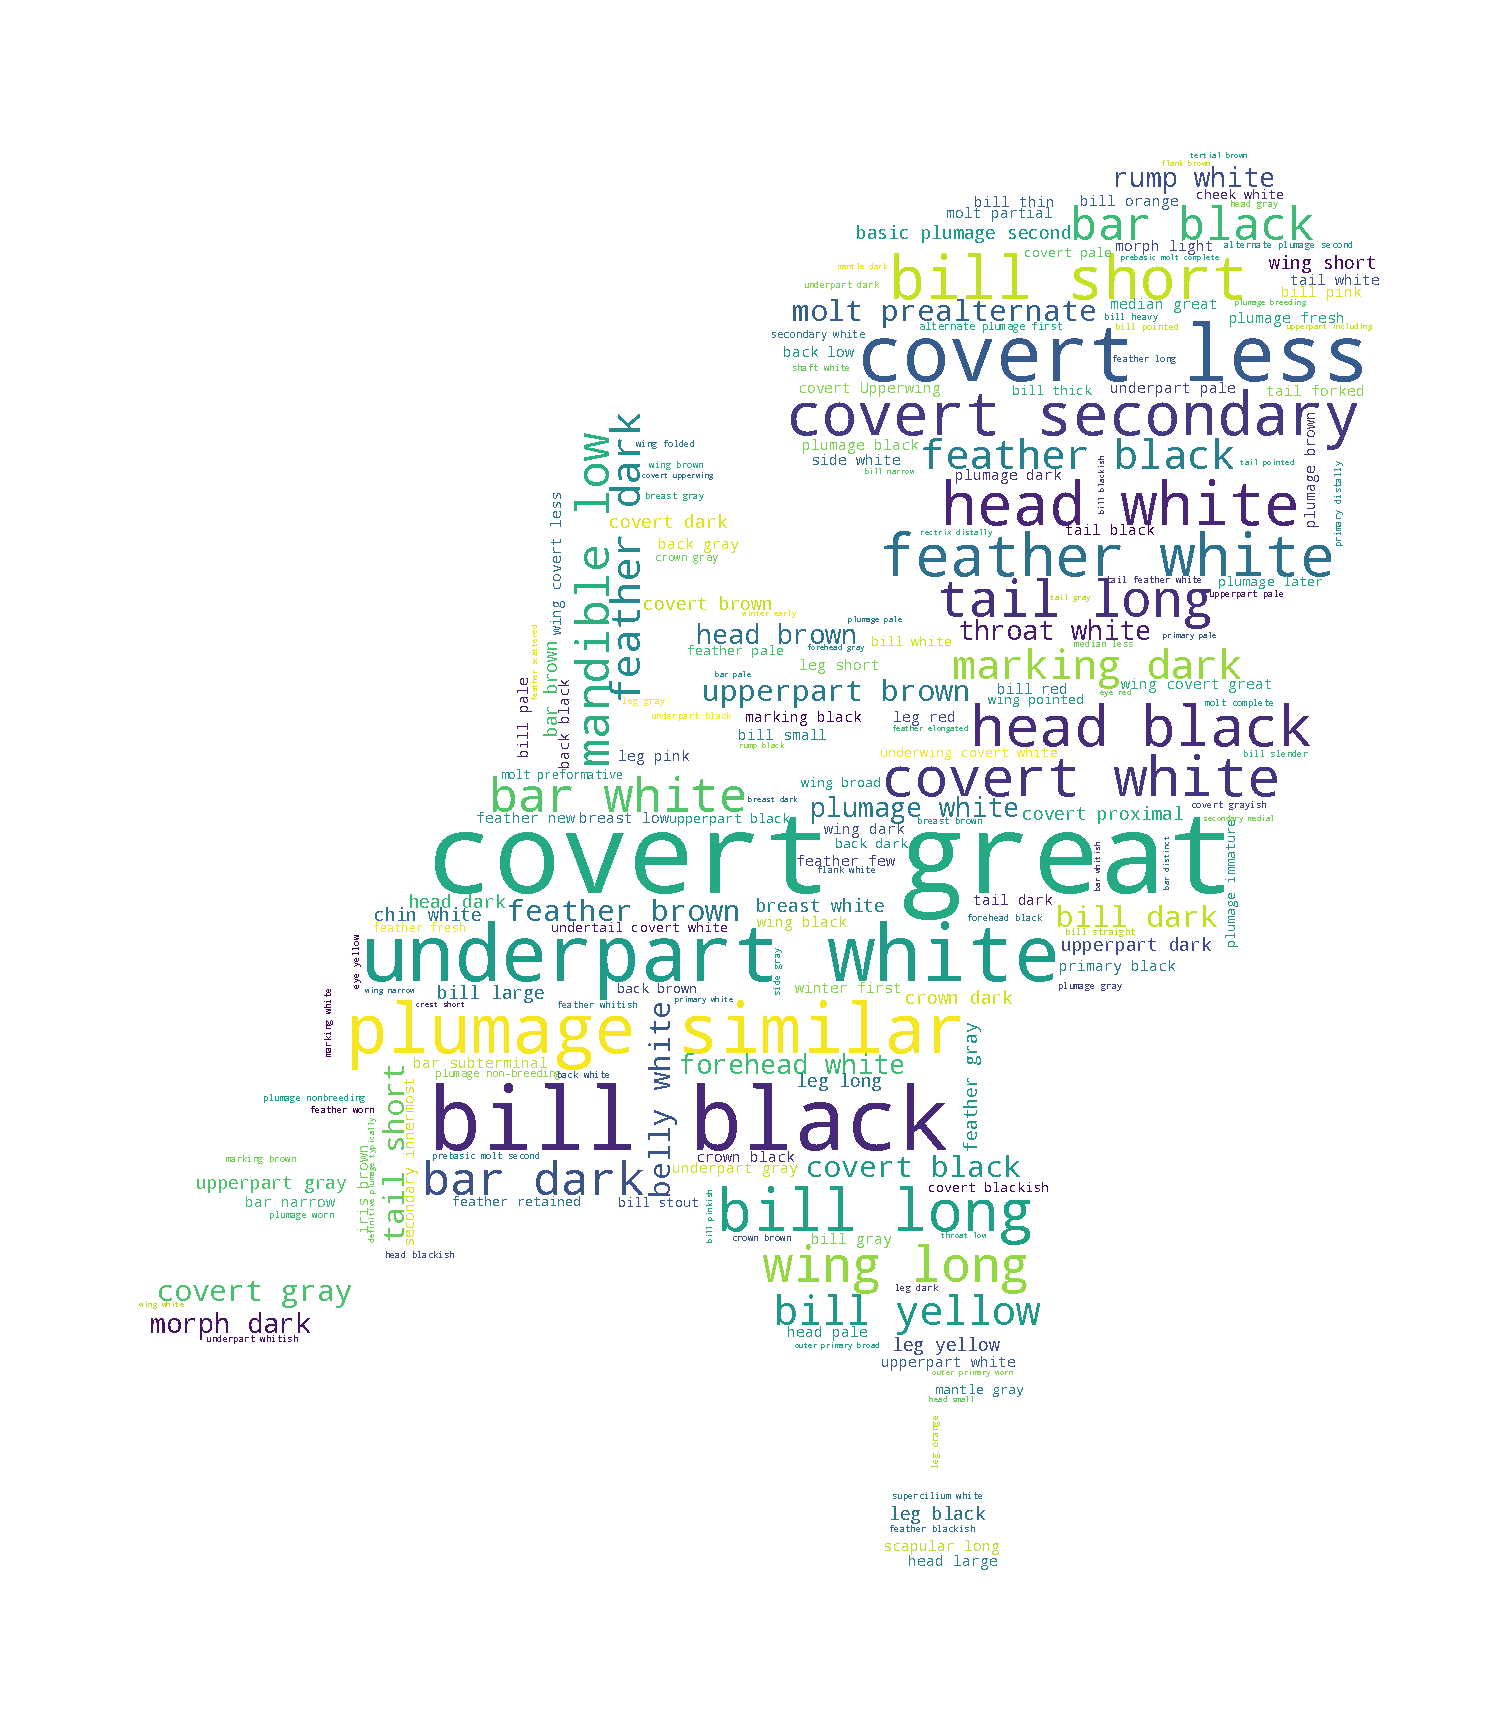
\includegraphics[%
    width=0.83\textwidth,
    %height=0.83\textwidth,
    align=t,
    smash=br,
    vshift=2.2cm,     % adjust the vertical position
    hshift=2.5cm     % adjust the horizontal position
    ]{figures/frontcover.pdf}%
  
  {\Large \theauthor}\vspace{6.0cm}
  
  \rotatebox{90}{\Large \thedate}\vspace{1.5cm}
  
  % This is the vector version of the new WUR logo; due to layout changes it visually looks larger than the old one
  \sloppypar{\vspace{0.0cm}\hspace{-2cm}
\includegraphics[width=13cm]{figures/WUR_RGB_standard.eps}}
  
  % Note: this image is not stretched out like it is in the MS Word template
  \sloppypar{\vspace{1.0cm}\noindent\makebox[\textwidth]{\hspace*{\dimexpr\evensidemargin-\oddsidemargin}
\includegraphics[width=\paperwidth]{figures/image2.jpeg}}}
  
  %%%%%% PAGE II 
  \restoregeometry
  \newgeometry{inner=1.91cm,outer=1.91cm}
  %\centering
  %\newgeometry{top=1.25cm,bottom=1.25cm,inner=0.66cm,outer=0.53cm,foot=1.19cm,includeheadfoot} % Subsequent page margins
  % Note: this uses the MS Word template margins, you might want to increase them a bit for printing (e.g. inner=1.91cm,outer=1.91cm)
  \thispagestyle{empty}
  
  \begin{center}
  {\bfseries \Large \thetitle}
  \newline
  \newline
  \newline
  \newline
  %{\bfseries \itshape Subtitle}\vspace{2.7cm}
  
  {\Large \theauthor}\vspace{0.25cm}
  
  {Registration number 920523897020}\vspace{2.5cm}
  
  {\large \underline{Supervisors}:}\vspace{.25cm}
  
  {Diego Marcos}
  
  {Ioannis Athanasiadis}\vspace{3.0cm}
  
  %{A thesis submitted in partial fulfilment of the degree of Master of Science}
  
  %{at Wageningen University and Research Centre,}
  
  %{The Netherlands.}\vspace{2.7cm}
  \end{center}
  
  \begin{center}
    {\thedate}
  
    {Wageningen, The Netherlands}
  \end{center}\vspace{5cm}

    Thesis code number: GRS-80400
  
    Thesis Report: GIRS-2022
  
    {Wageningen University and Research Centre}
  
    {Laboratory of Geo-Information Science and Remote Sensing}
 \end{titlingpage}
 \restoregeometry
\graphicspath{ {./figures/} }

\newpage
\thispagestyle{empty}
\section*{Foreword}
First of all, I would like to thank my supervisors Diego Marcos and Professor Ioannis Athanasiadis.
Both were always available for support and constructive criticism.
Especially Diego Marcos, without his feedback and constructive criticisms, this thesis would not have been possible.
\newline

\noindent
The front cover is a little joke to make the geo-information theme more prominent present in this thesis. 
Most of this thesis is about textual data without any location information.
The front cover is a word cloud that displays the most common Dutch bird traits that we found in our datasets. 
It contains 519 bird that are present in the Netherlands, somewhere we 'lost' 7 birds as according to the \href{https://avibase.bsc-eoc.org/checklist.jsp?region=NL&list=howardmoore}{Checklist of Dutch bird species} there are 526 birds (September 2020) present in the Netherlands.
For the word cloud we constructed a small database and simply counted the occurrences of all the trait combinations.
There are some mistakes such as 'Great Covert' obviously refers to 'greater converts' and does not mean that birds in the Netherlands have great coverts.  
While just used as a front cover, it does have some research potential to investigate the most common traits of a certain location.





\newpage
\thispagestyle{empty}
\section*{Abstract}
To tackle biodiversity loss, it is necessary to first identify and describe species.
By splitting a Deep Neural Network into a visual component and a natural language component, this process can be scaled and automated.
The natural language component first needs to learn to predict species based on visual traits.
This study aim to create a consistent database that contains morphological species trait, that can be used to learn a natural language processing model reason like a skilled taxonomist.

The first step is training an separate deep learning model that can recognise descriptive text about species.
This classifier is inserted into a web crawler and can automatically query species a retrieve descriptions about said species.
The result of running the web crawler for two weeks is a large database with textual descriptions for about 15,000 species.

The second step is extracting the most important and most descriminative traits per parts per species.
Several posthoc deep learning explanation techniques and part-of-speech in combination with dependency parsing are compared.
Part-of-speech in combination with dependency parsing extract the most relevant information from the descriptive sentences.
By matching sentences against a glossary containing expert words, misclassified sentences and irrelevant traits could be filtered out.
The data is processed and per species a knowledge graph is created.

Finally, a natural language processing model is training that can reason like a skilled taxonomist.
The model is trained on the knowledge graph that were reconstructed into small sentences before feeding them to natural language processing model.
This deep learning model is able to distinguish descriminative traits for the subset of species it has been trained on

\vspace{5mm} %5mm vertical space
\noindent
{\bf Keywords:} Natural Language Processing, Deep Learning, Species Classification, Knowledge Graph 


\glsaddall\printglossary[type=\acronymtype, nonumberlist]
\thispagestyle{empty}
\printglossary[nonumberlist]


\thispagestyle{empty}
{\hypersetup{linkcolor=black} 
\tableofcontents 
}
\thispagestyle{empty}
{\hypersetup{linkcolor=black} 
\listoffigures
}
\thispagestyle{empty}
{\hypersetup{linkcolor=black} 
\listoftables
}
\thispagestyle{empty}
\newpage


\newgeometry{top=2.8cm,bottom=2.8cm,inner=2.8cm,outer=2.8cm,}
\renewcommand{\thesection}{\arabic{section}}
\pagenumbering{arabic}

\section{Introduction}
\markboth{Introduction}{Introduction}

Estimated is that 50\% of the species are yet to be discovered, and many species will go extinct before ever being described \autocite{lees_species_2015}.
Scalable technologies that can help monitor diversity and help discover new species are more needed than ever. 
Deep neural networks (DNNs) can help discover new species, automate and speed up this process \autocite{van_horn_inaturalist_2018}.
However, DNNs are quite rigid, and their black-box behaviour could raise issues as it hampers the trustworthiness of the models \autocite{carvalho_machine_2019}.
It is essential to get more insights into the reasoning of a deep learning model in sensitive fields like taxonomy.
This way, we can learn a DNN to reason like an experienced taxonomist when describing existing and new species.

Many studies have already stipulated the importance of biodiversity for human life \autocite{pimentel_economic_1997, gowdy_value_1997, raffaelli_links_2010, joppa_biodiversity_2011, pimm_how_2018}.
With the current extinction rate, over 50\% of the species will be gone before the are ever discovered \autocite{lees_species_2015}.
Protecting biodiversity is now more needed than ever.
However, we cannot conserve undiscovered species; we first need to describe them to protect them \autocite{joppa_biodiversity_2011}.
This is where DNNs come in place.
DNNs can help discover new species and speed up the identification process \autocite{van_horn_inaturalist_2018}.
However, many species look alike.
They are difficult to distinguish and are easily misclassified, especially with less abundant species.
When a model now misclassifies a species, it is now difficult to check and correct the reasoning of that model.
We need a better understanding of how a DNN identifies and classifies species. 
This way, a less rigid DNN can be created, the results of the DNN can be interpreted more easily, and the results can be improved.

DNNs allow for remarkable performance in applications: from the automatic classification of text and images, natural language processing (NLP), to reinforcement learning.
DNNs outperform most classic machine learning approaches \autocite{he_delving_2015, brown_language_2020}.
The key to their success is end-to-end training.
Unlike classic machine learning models, deep learning models can automatically extract features needed for detection or classification.
Domain knowledge, in combination with careful engineering to extract the necessary features for the detection or classification, is no longer needed \autocite{lecun_deep_2015}.
However, end-to-end training also results in DNNs that are rigid, difficult to interpret and explain.
To extract the features from the input data, deep learning models use multiple neurons that take the input, process it to a slightly more abstract representation and pass it through the next layer of neurons \autocite{schmidhuber_deep_2015}.
Provided enough layers are stacked upon each other, very complex features can be extracted and correctly detected or classified by such a network (see Figure \ref{fig:CNN}, where a Convolutional Neural Network (CNN) takes in an image and makes a prediction based on its updated parameters.)
\begin{figure} [tbp]
    \centering
    \vspace{0cm}
    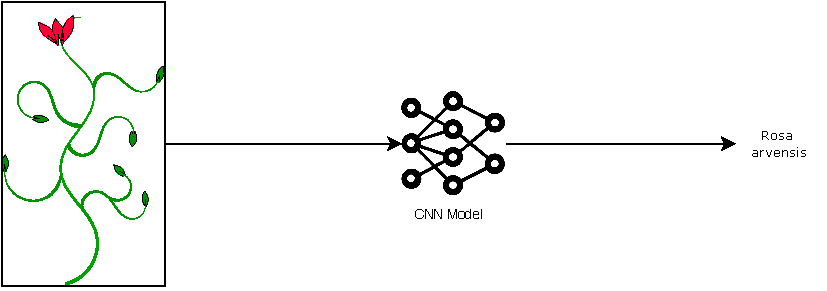
\includegraphics[width=\textwidth]{figures/CNN.pdf}
    \caption[Classic CNN]{A classic CNN approach, where the model takes the entire image as input and makes a prediction (based on the probabilities). The model uses several stacked layers to extract the features of the image. The output is correct, but the reasoning behind the prediction is hard to track.}
    \label{fig:CNN}
\end{figure}

Because the network's parameters are updated based on its input data, the reasoning of DNNs remains challenging to understand \autocite{li_interpretable_2021, losch_interpretability_2019}, and they do not perform well on long-tailed datasets\footnote{Long-tailed datasets are skewed datasets. A lot of samples are available for a few species and most species only are represented in the dataset only by a few species.}, like most real-world datasets \autocite{van_horn_inaturalist_2018}.
Stacking multiple layers of neurons on top of each other often results in millions of parameters.
All of these neurons use non-linear activation functions that decrease the interpretability of the network.
In long-tailed datasets, the parameters are not well optimised for less represented classes as the neurons cannot extract the necessary features.
While this automatic feature extraction is very convenient, it will become difficult to track models' reasons, and it can hamper performance.


Different algorithms and techniques have been proposed to increase the interpretability of the models.
Common approaches are feature reduction algorithms \autocite{ribeiro_why_2016}, inference of training sample contribution \autocite{koh_understanding_2020}, adding jittering to test samples and seeing how the prediction changes \autocite{li_understanding_2017} and decomposition and partial derivatives techniques \autocite{samek_explainable_2017}.
These algorithms and techniques all rely on posthoc explanations; they try to interpret an already trained DNN and explain its decisions a posteriori.
They try to identify important features via attributions \autocite{zintgraf_visualizing_2017, selvaraju_grad-cam_2017} or assign meaning to features \autocite{fleet_visualizing_2014}.
While some advances have been made in model understanding, giant leaps forward in the field of explainable AI remain limited \autocite{lipton_mythos_2017, li_interpretable_2021}.
These approaches might explain some of the inner workings of a DNN, but they do not help reason a DNN like a taxonomist.
The models remain rigid, and the intermediate results still remain challenging to interpret.
Designing models that are inherently interpretable by design are a better solution as these models do not give a false sense of trustworthiness \autocite{rudin_stop_2019}.

An a priori approach entails designing an architecture network with a semantic bottleneck layer that is interpretable for humans \autocite{bucher_semantic_2019}. 
The bottleneck layer is usually an intermediate layer fitted between a regular deep learning architecture \autocite{bucher_semantic_2019}.
The DNN is still trained end-to-end, but humans can inspect this semantic bottleneck layer to check the intermediate results.
In the case of a visual semantic bottleneck layer, things like colours, shape and texture are usually chosen as these can be semantically expressed and, they are overall important for classification or detection \autocite{yosinski_understanding_2015, fleet_visualizing_2014}.
Although all downstream results are based on this layer (i.e. all data has to flow through it), it does not hamper the results \autocite{bucher_semantic_2019}.
The semantic bottleneck layer allows deep learning developers to adjust the architecture more easily if the model does not perform as expected.

\begin{figure} [tbp]
    \centering
    \vspace{0cm}
    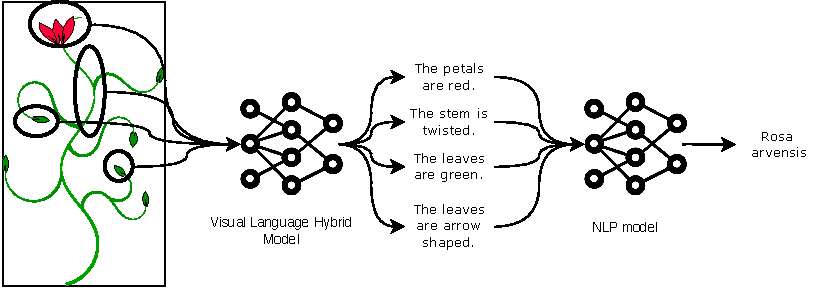
\includegraphics[width=\textwidth]{figures/architecture_v2.pdf}
    \caption[Proposed architecture]{The proposed architecture by \textcite{ishikawa_contextual_2021} for species classification. The model input is an image. The first model will describe the attributes present in the image in natural language. The second model will take the output of the first model and will make a prediction. The intermediate results remain interpretable using natural language and allow for shared traits among species.}
    \label{fig:intro}
\end{figure}

\textcite{ishikawa_contextual_2021} extended this bottleneck layer architecture by training a model that first learns the intermediate results.
The intermediate results are, in this case, similar to the semantic bottleneck.
The model is first trained to predict results in a human interpretable semantic way.
A second model will take these intermediate results to make a final prediction.
A more explainable, less rigid model for species classification might be created by extending the concept of the semantic bottleneck layer from \textcite{ishikawa_contextual_2021}.
A regular convolution neural network (CNN) for image classification is split into two separate models that communicate using natural language.
The first model will describe species features and traits present in the image of a species, and the second model will take these descriptions and infers the species (see Figure \ref{fig:intro}).
This way, DNNs' reasoning for species classification can be tracked, mistakes can be spotted, and the models' performance can be improved.

The first model will be a visual-language model that extracts the species' attributes from an image and describes its results in natural language. 
This vision hybrid model will be based on the research  of \textcite{radford_learning_2021} and \textcite{huang_interpretable_2020}.
Their findings allow the first model to learn to extract information from images by looking at raw text data that comes with image captions and describe objects present in those images.
This visual-language hybrid model will describe learned species attributes and use zero-shot learning to describe unseen (new) distinctive species traits.
By first describing traits, less abundant species can benefit from more abundant species if they share common traits.
This allows to model to perform better on long-tailed species datasets \autocite{van_horn_inaturalist_2018}.
Each species present in the dataset will be described equally well because the DNN can learn traits from more abundant species.
The second model is a pure natural language processing (NLP) model that takes the partial descriptions and infers the species.
This way, a models reasoning for species predictions might be tracked by investigating the intermediate results \autocite{ishikawa_contextual_2021} and the final model results will be less rigid.

By first training the NLP model, we can create a model that can infer species based on partial textual descriptions. 
As DNNs need large datasets to properly learn the necessary features from the data \autocite{xue-wen_chen_big_2014, gheisari_survey_2017}, we first need to create this dataset.
This dataset needs as many unique descriptions as possible for each species, so for both a taxonomist and the NLP model, it would be possible to infer the species name based on provided descriptions.
We expect that a DNN model will learn the most important traits of a species if we can feed it enough unique descriptions.
For example, suppose the model sees multiple unique sentences about a European robin (also see Figure \ref{fig:workflow}) containing the same information.
The model will learn that an important trait for a European robin is its orange breast and plumage.
By applying posthoc explanatory techniques, we can extract the most discriminative features from the text used for making a prediction.

The first objective of this research is to create a high-quality database with species and their descriptions.
The following research question accompanies this objective:
\begin{itemize}
    \item \emph{How can a high-quality database be created containing species names and a combination of unique descriptions per species?}
\end{itemize}
We will train a model that can recognise descriptions sentences and deploy this model in a web crawler that can automatically query search engines.
The text from the returned URLs are broken down into single sentences, and the model classifies the sentences.
We hypothesise that this will result in a large database with clean descriptions,
that an NLP model can use to learn distinctive features per species.

We want to process these sentences to extract the most important words per sentence, resulting in a large database with the most important traits per species.
The second objective of this research is: to process the data in such a way that only the most relevant parts of the sentences are stored:
\begin{itemize}
    \item \emph{Which interpretation techniques can be used with the descriptive sentences to extract the most relevant traits for a species?}
\end{itemize}
We train an NLP classification model on the sentences and expect the classifier to focus on the most important traits.
We compare several posthoc explanation techniques to retrieve keywords. 
Besides the method above, we also use the pre-trained transformer model of \textcite{wolf_huggingfaces_2020} to extract the necessary features, as these models are already pre-trained to extract relations between words.

Finally, we investigate how we can train an NLP model that can infer species based on the data we gathered and processed:
\begin{itemize}
    \item \emph{How should a deep learning model be built, trained and evaluated to predict existing species with natural language?}
\end{itemize}
This model should distinguish species based on the data from research objective two.
We expect that the model will (depending on the species used for training) distinguish species from each other and return the most distinctive feature(s) per species. 
The final result will be a clean database.
This database contains clean species descriptions, and there should be a distinction present to see which morphological trait is the most important.

We first will describe our approach in the Methodology in Section \ref{par:methodoly}.
Section \ref{par:dataset}, describes how we gather enough data to train an NLP model to recognise text descriptions an inn Section \ref{par:keywords} we describe a method for comparing different posthoc explanatory techniques to extract the most distinctive traits of each species.
Section \ref{par:species_prediction} we describe how we train and NLP model to infer species based on descriptions.
In Section \ref{par:results}, we present the results, and in Section \ref{par:discussion}, we discuss our results.

\newpage
\section{Methodology} \label{par:methodoly}
\markboth{Approach}{Approach}


\begin{figure} [htpb]
    \centering
    %\vspace{-2cm}
    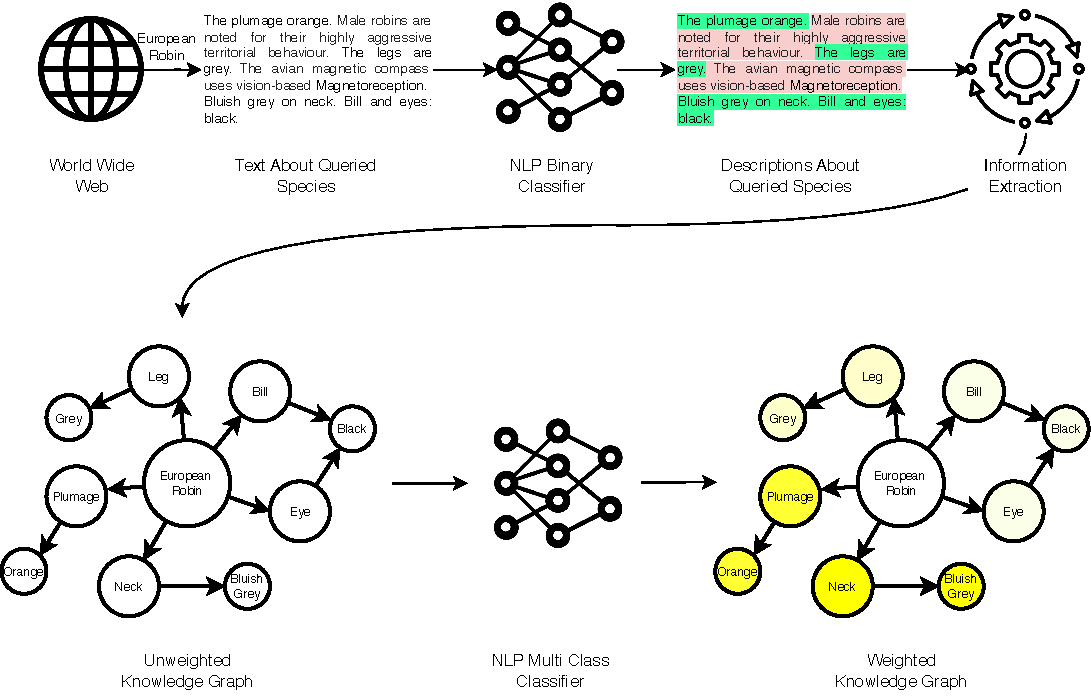
\includegraphics[width=\textwidth]{figures/workflow.pdf}
    \caption[Proposed Workflow]{A simplified proposed workflow for this thesis. The web crawler searches for species descriptions on the world wide web. We use a custom script combined with the transformer models of \textcite{wolf_huggingfaces_2020} to extract the information from the sentences and create a knowledge graph per species. Finally, an NLP model is trained to extract the most distinctive traits of the knowledge graph that make a species distinct from other species.}
    \label{fig:workflow}
\end{figure}

The core of our idea is gathering enough text data per species so that an NLP model can learn keywords describing each species.
Using natural language for this idea has several potential benefits.
Humans communicate using natural language, resulting in a theoretically endless amount of data that can be used, and by using natural language, the results remain interpretable for humans.
We first create a DNN that can classify species descriptions and deploy this DNN in a web crawler.
This web crawler can automatically query species and store descriptive sentences.
We use the harvested data to train the NLP model.
Finally, we assess the NLP model.
In Figure \ref{fig:workflow}, a simplified version of the workflow can be found.
This chapter will give a detailed description of the steps.

\subsection{Gathering Species Descriptions} \label{par:dataset}
The World Wide Web has potentially an endless amount of species descriptions available, making the internet suitable for harvesting training data.
However, description sentences can be theoretically limitless, e.g. for a Brown bear (Ursus arctos), the description text could be: "The fur is brown", "The brown bear has brown fur".
These are relatively simple sentences.
Sentences can also have a more difficult semantic, e.g. "The fur of the Brown bear is similar to that of the Grizzly bear".
A classic machine learning approach that requires a rule-based match system for sentence classification is not feasible to harvest description data from the internet.
Instead of a classic rule-based approach, we train a DNN to classify text into description or non-description.
A large, accurate, and consistently labelled dataset is needed to properly train a deep learning model that can classify text data into description text and non-description text \autocite{munappy_data_2019, minaee_deep_2021}.

\subsubsection{Training a Model for Text Classification} \label{par:reedloss}
%The internet has a vast amount of free data available that can be easily harvested.
We create this large dataset by scraping text from structured web pages.
We select three websites that have large databases, are structured enough and have rich scholarly content about species:
\begin{itemize}
    \item \href{www.wikipedia.com}{Wikipedia}. Wikipedia is a free online encyclopedia that volunteers maintain. Everyone is allowed to edit pages. Moderators and other volunteers maintain quality.
    \item \href{https://birdsoftheworld.org/bow/home}{Birds of the World (BoW)}. BOW is constructed and maintained by ornithologists worldwide \autocite{billerman_birds_2020}.
    \item \href{https://powo.science.kew.org/}{Plant of the World Online (PoWO)}. PoWO is an international collaborative database of the world's flora. Its data is based on scientific papers. It is maintained by the Royal Botanic Gardens \autocite{facilitated_by_the_royal_botanic_gardens_plants_2019}.
\end{itemize}
All three websites divide their information into paragraphs such as "Introduction", "Appearance", "Characteristics", "Habit".
These headers allow us to automatically label large amounts of data with a few lines of code.
We store the text from paragraphs with titles like "Introduction" and "Habit" as negative labels and "Characteristics" and "Appearance" as positive values, making this a two-class classification problem (see Appendix \ref{app:key_words} for the complete list per database).
The text chunks inside the paragraphs are used as features.
Random pages from Wikipedia that are not about species are also used to gather additional negative values.
We hypothesise that the model will better classify text not related to species descriptions.

%\subsubsection{Tokens & Tokenisers} \label{par:Tokens}
%NLP models process text.
%To process words, sentences or even complete chapters, they first need to be converted to number, i.e. tokens.
%BERT models use two specials tokens.
%This first token is always \verb|[CLS]|, which stands for "Classification".
%Using \verb|[CLS]|, the model knows the sequence is used for classification.
%The second token is \verb|[SEP]|, which stand for "Separation". 



\subsubsection{Model Architecture} \label{par:Architecture}


\begin{figure} [htpb]
    \centering
    %\textbf{The Web Crawler}
    %\vspace{-2cm}
    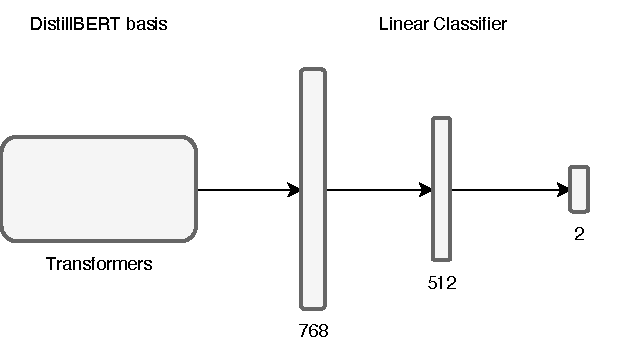
\includegraphics[width=0.6\textwidth]{figures/architectureDL.pdf}
    \caption[Model Architecture]{The model architecture. We use the distilled BERT bases of \textcite{sanh_distilbert_2020} and fit a linear classifier on top of it.}
    \label{fig:model_architecture}
\end{figure}

As a base for the text classification model, we used a distilled version (distillBERT) of the Bidirectional Encoder Representations from Transformers (BERT) \autocite{devlin_bert_2019}, created by \textcite{sanh_distilbert_2020}. 
This version of BERT is 60\% faster, has 40\% fewer parameters and still reaches 97\% on general language understanding \autocite{sanh_distilbert_2020}.
Using a pre-trained model can provide significant improvements over models trained from scratch \autocite{mikolov_distributed_2013}.
The use of a pre-trained model is called transfer learning and could speed up the training process and increase the accuracy of the deep learning model.
Both distillBERT and BERT are already trained on a large corpus of English words and can be used freely.
\textcite{sun_how_2020} have already investigated how to fine-tune BERT for text classification.
We use their findings on the full BERT model to fine-tune the distilBERT model for description text classification.

Like \textcite{sun_how_2020}, we first fit a dropout layer (0.1) on top of the distillBERT architecture to enable regularisation.
This dropout layer is followed by a Rectified Linear Unit (ReLU) activation function:
\begin{equation} \label{ReLU}
    f(x) = \max(0, x)
\end{equation}
The ReLU activation function is followed by two fully connected layers.
The first linear layer has an input size of 786 (BERT and distillBERT both output a vector of 768 for each token) and output size of 512.
The second linear layer has an input size of 512 (output of the first linear) and an output of 2, as this is a binary classification problem.
The final activation function is a log-likelihood (log-softmax) function:
\begin{equation} \label{eq:logsoftmax}
    f(x) = \log_{}(\frac{e^{x_i}}{\sum_{j=1}^K e^{x_j}})
\end{equation}
Where~$x$ is the~$log$ probability.
Using a log-softmax will slightly increase the error factor of the model over a normal softmax function, punishing mistakes a bit higher.
he standard likelihood (softmax) probabilities can be computed by taking the exponent:
\begin{equation}
    p = e^{x} 
\end{equation}
Where~$p$ is the probability value between 0 and 1 and~$X$ is the output of the log-softmax layer.

The basis distillBERT architecture can be fine-tuned further by updating the inner parameter of the transformer layers during training. 
This can be useful if BERT is utilised in the non-general domain \autocite{devlin_bert_2019, sun_how_2020, sanh_distilbert_2020}, which is the case with description data.
However, we decided not to fine-tune the inner workings of BERT for two reasons: 
(1) We used additional Wikipedia to increase the text data with negative values.
These random Wikipedia pages are highly likely to contain information from the public
domain, resulting in a  data distribution close(r) to the public domain.
(2) A binary classification problem is a relatively simple task; updating the inner parameters during training costs additional time and computing power, while it only might result in a slight accuracy increase.

To prepare the text spans, we use the tokeniser of \textcite{wolf_huggingfaces_2020}.
The used BERT architecture can only process up to 512 tokens at once \autocite{sanh_distilbert_2020, devlin_bert_2019}.
Most tokenisers will truncate text spans larger than 512 tokens as most text information is at the beginning (head-encoding), end (tail-encoding) or beginning and end (head+tail-encoding).
We decide not to truncate the text.
Instead, we randomly split the text into text spans with a minimum of 10 words and a maximum of 512 words.
We hypothesised that the model might be better in recognising shorter description spans by splitting the raw spans, while it can still recognise larger spans in the meantime.  
This way, we enlarge the dataset and prevent losing information with truncating spans larger than 512 tokens. 
We use a minimum of 10 words to prevent the model from fixating on specific words.

%The tokeniser of \textcite{wolf_huggingfaces_2020} returns a Python dictionary with the input ID's and the attention mask of the text.
%E.g. by tokenizing the text "This is a test.", the tokeniser returns the following:
%~$'input\_ids': [101, 2023, 2003, 1037, 3231, 1012, 102]$, 
%~$'attention\_mask': [1, 1, 1, 1, 1, 1, 1]$.
%~$[101]$ indicates the start of a sequence and ~$[102]$ indicates the end of a sequence.
%During the training the text is also padded to the maximum of 512 tokens and the attention masks are randomised between 0 and 1.

\subsubsection{Loss Function}
Automatically labelling the data will not result in a consistent dataset.
There is a chance we miss pecific headers and mislabel them during the preprocessing.
Even if we correctly label all features, not all data will be labelled correctly as text is generally unstructured \autocite{kumar_text_2020}.
E.g. some species descriptions might be located in the paragraph "Introduction", and some general information might be in the paragraph "Characteristics".
Consider the text "The European robin is red-breasted with distinctive eyes.".
This text is likely to be found in a paragraph about descriptions.
However, it is also possible that such a piece of text occurs in another paragraph like the introduction, or it could even be part of an image caption of an entirely different paragraph. 
In these aforementioned cases, the piece of text will be mislabelled and will result in a messy dataset.
By implementing the semi-supervised loss function from \textcite{reed_training_2015}, we can correct the inconsistency of the dataset:
\begin{equation} \label{eq:softloss}
 SoftLoss(q, t) = \sum_{k=1}^{L}[\beta t _k + (1- \beta )q _k]log(q _k)
\end{equation}
Where~$q$ is directly used to calculate regression targets for each batch,~$t$ is the target value, and \(\beta\) is used to balance the prediction.
Using natural language in combination with the soft loss function from \textcite{reed_training_2015} allows the model for semi-supervised learning.
This combination has the advantage that it is now very easy to scale natural language training as we do not need to hand annotate the datasets.
With Equation \ref{eq:softloss}, the model is now 'allowed' to disagree with the training label to a certain extent when the prediction certainty of the model is high enough.
%When the prediction values reach a set threshold (\(\beta\)), the prediction is treated as correct and the loss is calculated accordingly.
%If the model prediction reaches the set threshold, the prediction is seen as a the correct label and the label is changed during the training process, but if the model prediction is below the threshold, the loss will be calculated accordingly.
We assume most labels are correct, allowing the model to learn enough from these samples.
Therefore we use a \(\beta\) of 0.80\footnote{Best practice would be find the correct \(\beta\) through cross validation \autocite{reed_training_2015, han_survey_2021}. However, as we train the model on Google Colab instances this would not be feasible.}.
If we start with a low \(\beta\) (e.g. 0.50), there is a chance the model does not learn correctly as it can bootstrap too many samples.
If we use a high \(\beta\) (e.g. 1,00), the model cannot bootstrap any samples, resulting in a regular cross-entropy loss.

\subsubsection{Training \& Evaluation}
%We train the model on a Google Colab instance.
We use the Adam optimiser \autocite{kingma_adam_2017} during the training process.
The Adam optimiser has shown good performance when fine-tuning BERT for text classification \autocite{you_large_2020}.
The hyperparameters were set based on the paper of \textcite{sun_how_2020}.
The learning rate was set to 3e\textsuperscript{-5}, and the batch size was set to 32, as this is generally found to be the most effective batch size for BERT \autocite{devlin_bert_2019, sanh_distilbert_2020, sun_how_2020, you_large_2020}.
We clip the gradients to prevent them from exploding. 
We train the model for 35 epochs.

As there is a high probability that the dataset is will be unbalanced, we will evaluate it with a precision-recall summary and a precision-recall curve.
The precision-recall summary and curve give more reliable results with unbalanced datasets \autocite{saito_precision-recall_2015}.
When the model reaches an F1-score of at least 0.90 on the test set, the model is tested on two additional held-out databases, the \href{http://www.llifle.com/}{LLifle} dataset and the \href{https://www.worldagroforestry.org/}{AgroForestry} dataset.
When the model reaches an F1-score of 0.80 on these external datasets, the model will be deployed in a web crawler.
The F1-score is calculated with the following formula:
\begin{equation}
    F_1 = 2 \cdot \frac{\mathrm{precision} \cdot \mathrm{recall}}{\mathrm{precision} + \mathrm{recall}} 
\end{equation}
We use the Python package from \textcite{pedregosa_scikit-learn_2011} to calculate precision-recall metrics.

Before text tokenisation, we first clean it of references and footnotes.
We no longer split the into random chunks, but we use a sentecizer of \textcite{honnibal_spacy_2020} to split the text into sentences.
Splitting text into sentences instead of random text chunks prevents information loss.

The held-out datasets will also have mislabelled sentences like the training data.
We use the following equation\footnote{This actually looks like the \texttt{hardloss} (Equation 7) from \textcite{reed_training_2015}. In this case the equation is changed from a loss function to an If-Then statement.} to correct these labels to a certain extent:
\begin{equation} \label{eq:softloss_ifthen}
(\hat{\gamma}^{(i)} >= \beta \rightarrow \hat{\gamma}^{(i)} = \gamma^{(i)}) \wedge ( \leftharpoondown \hat{\gamma}^{(i)} = \hat{\gamma}^{(i)})
\end{equation}
Where~$\hat{\gamma}^{(i)}$ is the predicted value,~$\gamma^{(i)}$ is the actual label and~$\beta$ is the set threshold. 
As the loss is no longer calculated, we simply calculate the prediction certainty of the model.
If the model reaches a probability of 0.80 or higher (\(\beta\)), the model is allowed to change the label; in all other cases, the predicted label is matched against the actual (paragraph) label.


\subsubsection{Gathering \& Storing Description Data}
We deploy the classification model in a web crawler.
This web crawler can automatically query search engines with a predefined list of birds and plants.
The list for plants is based on the \href{https://www.ipni.org/}{International Plant Name Index} (IPNI), and the list for birds is based on the BoW database. %of \href{https://birdsoftheworld.org/bow/home}{Birds of the World} (BoW).
The IPNI database contains over 1,3 million plant species, and the BoW database contains over ten thousand birds.

The IPNI database is extensive, containing all 1,3+ million known plant species.
%There is a high chance that not all species in this database can be queried within the time-frame of this research.
It is unlikely to query all species. 
Therefore we sort the plant species based on their descriptions in the PoWO dataset used to train the classifier.
Plant species with more descriptions also have a higher chance of being described somewhere else on the web.
This way, we make sure the plants that will be queried have a high chance to contain a description somewhere on the web.
We do the same for the bird species; bird species are sorted based on their number of descriptions in the BoW dataset.

%The web crawler queries the search engines. 
%This results in a list URLs with possible species descriptions.
\begin{figure} [t]
    \centering
    %\textbf{The Web Crawler}
    %\vspace{-2cm}
    \makebox[\textwidth][c]{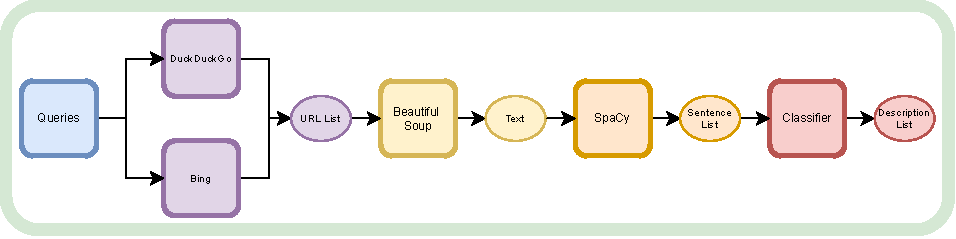
\includegraphics[width=\textwidth]{figures/webcrawler.pdf}}
    \caption[Web Crawler]{The process of the web crawler. The search engines are queries with five different queries per species. The search engines return a list of URLs per species. BeautifulSoup break extract the HTML of each URL and retrieves the text. SpaCy break the text down into single sentences. The sentences are presented to the classifier.}
    \label{fig:webcrawler}
\end{figure}

\begin{figure}[htpb]
    \centering
    
    \begin{subfigure}[b]{1.00\textwidth}
        \centering
          \framebox{\parbox{\dimexpr\linewidth-2\fboxsep-2\fboxrule}{%
          "Plumage, legs and beak orange. The bill and the legs are both black. The house is large with enormous windows. This is something random, but the sexes are similar. Nuclear power might solve the world's energy crisis. The tree has a brown bark and the leaves are pointed. The trunk bears conical spines to deter animal attacks. By growing in shaded places, the plant reduces evaporation. Seeds are 3 cm. Branches usually in whorls of 3."}}
        \caption{A random piece of text.}
        \label{fig:webcrawler_sents_nopred}
    \end{subfigure}
    \vfill
    \begin{subfigure}[b]{1.00\textwidth}
        \centering
        \framebox{\parbox{\dimexpr\linewidth-2\fboxsep-2\fboxrule}{%
        "
        \sethlcolor{color1}\hl{Plumage, legs and beak orange. < 0.585 >}
        \sethlcolor{color2}\hl{The bill and the legs are both black. < 0.943 >}
        \sethlcolor{color3}\hl{The house is large with enormous windows. < 0.045 >}
        \sethlcolor{color4}\hl{This is something random, but the sexes are similar. < 0.486 >}
        \sethlcolor{color5}\hl{Nuclear power might solve the world's energy crisis. < 0.026 >}
        \sethlcolor{color6}\hl{The tree has a brown bark and the leaves are pointed < 0.722 >}
        \sethlcolor{color7}\hl{The trunk bears conical spines to deter animal attacks. < 0.530 >}
        \sethlcolor{color8}\hl{By growing in shaded places, the plant reduces evaporation. < 0.162 >}
        \sethlcolor{color9}\hl{Seeds are 3 cm. < 0.964 >}
        \sethlcolor{color10}\hl{Branches usually in whorls of 3. < 0.999 >}
        "}}   
        \caption{A random piece of text broken down into single sentences and classified.}
        \label{fig:webcrawler_sents_pred}
    \end{subfigure}
    \caption[An example how the web crawler 'sees' the text data]{A small example how text from URLs is processed. Text is broken into single sentences by the Sentecizer of \textcite{honnibal_spacy_2020} and the classifier classifies each sentences. Sentences with a value of 0.50 or higher are stored in the database. The darker the colour green, the higher the prediction value. The prediction value is also shown after each sentence.}
    \label{fig:webcrawler_sents}
\end{figure}


We use five different ways of constructing a query: the species name without any additional search term and the species name plus 'description', 'diagnosis', 'attributes' or 'captions'.
We wrap quotations around the species to force the search engine to return the exact species name.
This way, search engines cannot return any results that it deems similar.
Each query will return a list of candidate URLs and are appended to a list for a single species.
%The URL list is checked for duplicates as this is computationally less expense than calculating the cosine similarity for each sentence to drop duplicates.
The URLs are visited, and all the text is retrieved.
If a URL points towards a PDF file er text file, it is skipped.
PDF files and text files are read line by line and not as a single text span, and it is difficult to break these down into single sentences. 
Finally, the header of the URL is checked against the queried species to make sure that the page contains information about the queried species.
In Figure \ref{fig:webcrawler}, the process overview of the web crawler can be found, and in Figure \ref{fig:webcrawler_sents}, a small example can be found of how the web crawler 'sees' a random piece of text.
Figure \ref{fig:webcrawler_sents_nopred} contains the unclassified text, and Figure \ref{fig:webcrawler_sents_pred} contains the classified text.
%Not every query will return correct websites, i.e. websites about the queried species.
%This way we prevent accidentally storing description data for the wrong species.

The raw text is retrieved and broken down into single sentences when the web page meets all criteria. 
This makes sure the descriptions will be stored as much as possible per unique species trait.
The text is cleaned using several regular expressions. % LINK TO THE EXPRESSIONS
We use a pre-trained sentecizer from \textcite{wolf_huggingfaces_2020} to split the text into single sentences.
Every sentence is checked against the train description classifier.
If the model recognises a description, the sentence is stored. 
We use a threshold of 0.5 to determine if a sentence is a description or otherwise.
In Figure \ref{fig:webcrawler_sents}, a small example can be found of how the web crawler will process web pages and stores relevant information. 




\begin{comment}


\begin{figure} [htpb]
     \centering
     \begin{subfigure}[b]{1.00\textwidth}
         \centering
         %\hspace{-1.0cm}
         \frame{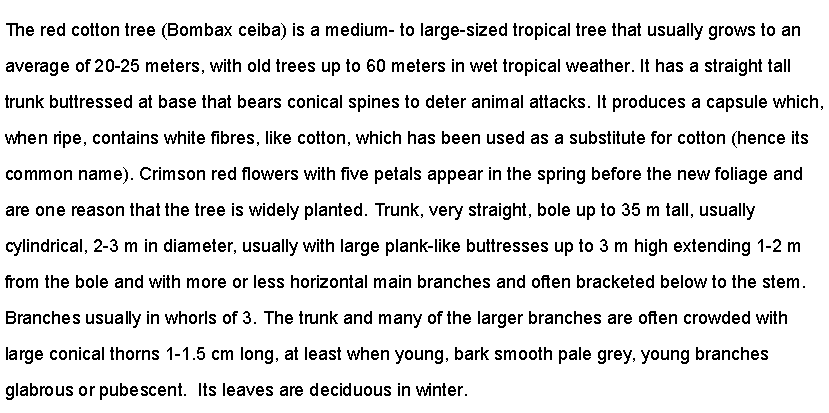
\includegraphics[width=\textwidth]{web_crawler_example_sents_2.pdf}}
         \caption[Raw text span example]{The raw text span from a web page. This a small portion of a web page about Bombax ceiba (source: \href{http://www.llifle.com/Encyclopedia/TREES/Family/Bombacaceae/31994/Bombax_ceiba}{Llilfe.com/Bomax\_ceiba}).}
         \label{fig:webcrawler_sents_nopred}
     \end{subfigure}
     \vfill
     \begin{subfigure}[b]{1.00\textwidth}
         \centering
         %\hspace{-0.5cm}
         \frame{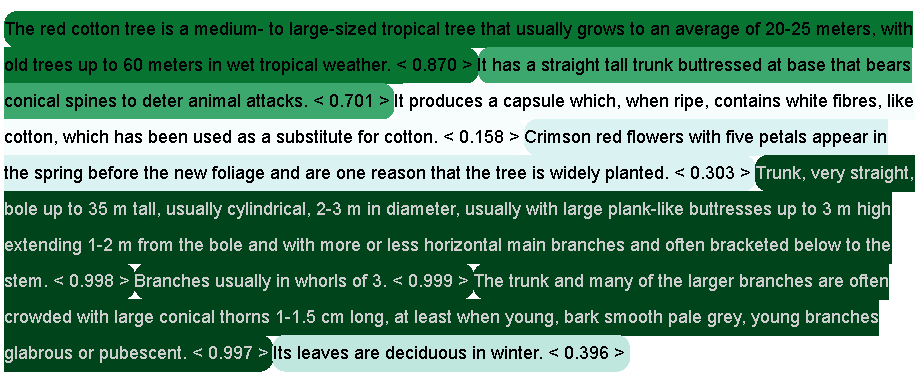
\includegraphics[width=\textwidth]{web_crawler_example_sents_preds_2.pdf}}
         \caption[Cleaned and classified text span example]{The cleaned and classified text. The text is coloured by the prediction value (high value is dark green, a low value near white). The prediction value of each sentence can be found at the end of the sentence.}
         \label{fig:webcrawler_sents_pred}
     \end{subfigure}
     \caption[Example of the web crawler process]{A small example how the web crawler processes and classifies data from a web page. The raw text span is cleaned from brackets, sources and other textual punctuation irregularities. After cleaning the text is split into single sentence. Each sentence is classified by the model. Sentences that reach or exceed the threshold of 0.5 are stored. Although this example is never seen by the model (not used in training), the classifier classifies the sentences with high certainty in most cases.}
     \label{fig:webcrawler_sents}
\end{figure}


\end{comment}
\begin{comment}

\subsubsection{Sentence Similarity}
There is a change that different web pages use the a common source for describing a species.
By checking for similar sentence within the same species we make sure the same sentence is not appended twice to the dataset and the train and test set are completely disjoint.
Like \textcite{reimers_sentence-bert_2019} we use the last hidden state of BERT (distilBERT in our case) and compute the cosine similarity to measure the distance between text spans.
Fortunately, this last hidden state is the output of a base BERT architecture.
However, the last hidden state output contain a matrix of 512 x 768. 
It is not feasibly to compute the cosine similarity distance for multiple matrices of this size.
By using a mean-pooling operation we create a vector of size 768 for every text span and compute the cosine distance for these text spans.
We first create a new dictionary that corresponds to the dictionary initialised by the tokeniser, \verb|{'input_ids': [], 'attention_mask': []}|.
We tokenise all the sentences we are comparing and append the tokens and masking to the correct key.
After all the sentences have been processed, we reformat the dictionary into a single tensor and push it trough the model.
This will result in a tensor of the number of sentences times 512 times 768. 
We sum the 3D matrix along the first axis, resulting in a 2D matrix.
The size of this matrix is the number of sentences time 768.
Each sentence is represented by a vector of size 768
Finally we calculate the cosine similarity between the sentences and drop sentences that exceed the threshold of 0.99.
In Figure \ref{fig:similarity_matrix} a comparison of a few fictional sentences can be found.
\begin{figure} [htbp]
    \centering
    \vspace{0cm}
    \hspace{-1cm}
    %\textbf{Similarity Matrix}
    \makebox[\textwidth][c]{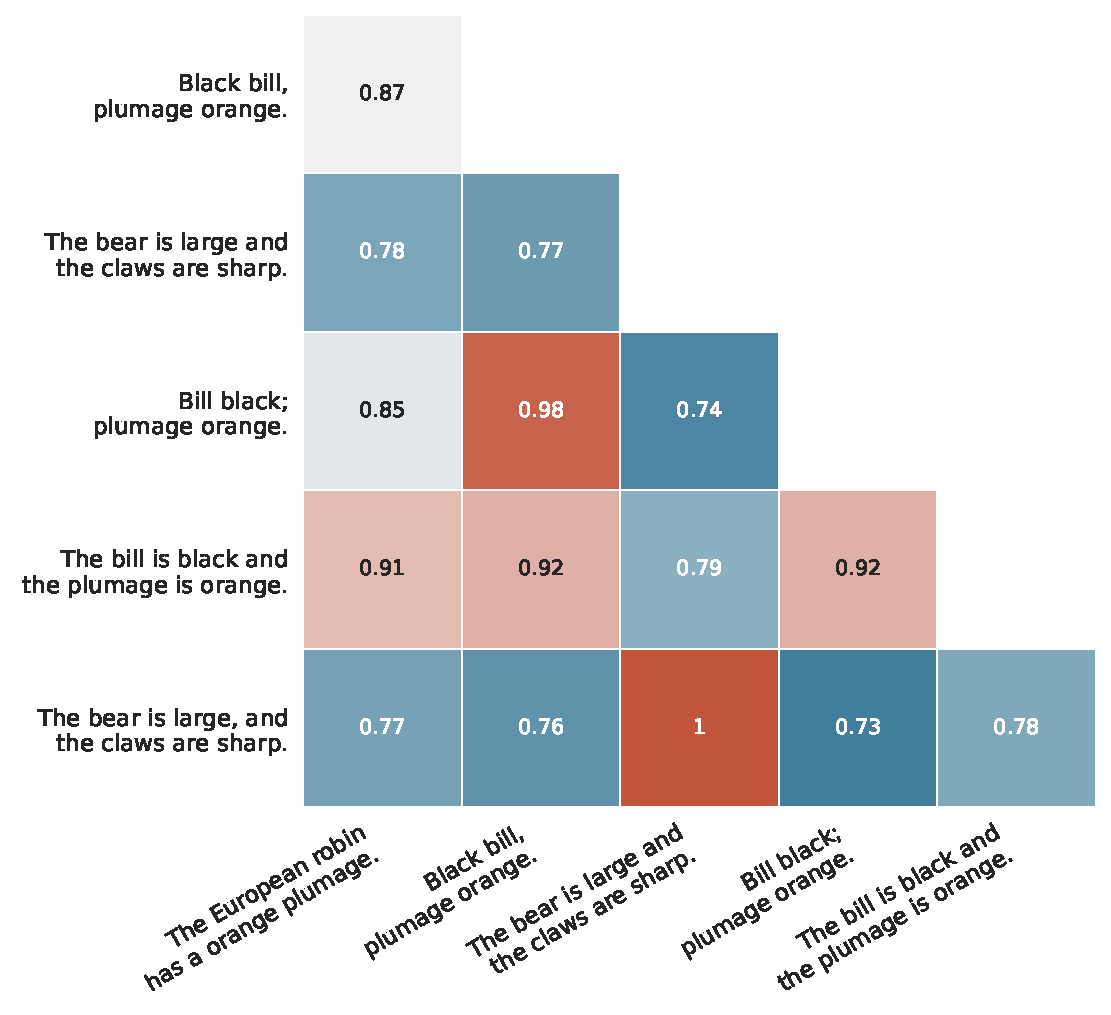
\includegraphics[width=0.7\textwidth]{similarity_matrix.pdf}}
    \caption[Example of sentence similarity]{An example for the calculation of sentence similarity. 
    %In this example the following sentences are compared.
     %0 - "The European robin has a orange plumage."
     %1 - "Black bill, plumage orange."
     %2 - "The bear is large and the claws are sharp."
     %3 - "Bill black; plumage orange."
     %4 - "The bill is black and the plumage is orange."
     %5 - "The bear is large, and the claws are sharp."
    In this case the sentences "Bill black; plumage orange." and "Black bill, plumage orange." reach a similarity score of 0.98. The word order and the punctuation is slightly different. In this case both sentences are stored in the database as it is highly likely they come from different sources. However in the case of "The bear is large and the claws are sharp." and "The bear is large, and the claws are sharp." the sentences are completely similar except for the punctuation. The sentences reach a similarity score of 1 (although this will be because of rounding). In the second case the sentences will come from a the same source and one of them will not be stored.}
    \label{fig:similarity_matrix}
\end{figure}

%Some databases store their description as one long sentence, describing multiple attributes in a single sentence e.g. "Leaves 5–9-foliolate; leaflets narrowly elliptic-obovate, entire, acuminate, 7–20 x 1.8–6.5 cm, glabrous; petiole 5.5 - 25 cm long, at the apex expanded into an almost circular disk." (source: \href{http://powo.science.kew.org/taxon/urn:lsid:ipni.org:names:1166232-2}{PoWO/Ceiba\_pentandra}). 
%This sentence is describing the leaves and the attributes in the same sentence. 

\subsubsection{Knowledge Graph}
A knowledge graph (KG) is a graph that contains interlinked descriptions, information has a formal structure that allows both people and computer to process the data unambiguously \autocite{petkova_crafting_2020}, like in Figure \ref{fig:graph_example}.
If we apply this to species descriptions we would expect the end up with a single graph per species, or with a large graph per class (e.g. mammalia).
Traits are not longer unique and can be shared per species.
Processing the data this will will result in a clean semantic database for both humans and computers.
This database will only contain subjects, relations and objects, also known as semantic triples. 
When feeding this data to the model it cannot be become dependent on artefacts such as word order, punctuation's, etc.

\begin{figure} [htpbtb]
    \centering
    \begin{subfigure}[b]{1.0\textwidth}
        \centering
        %\vspace{0cm}
        \includesvg[inkscapelatex=false, width=\textwidth]{PoS_example.svg}
        \caption[Example of part of speech tagging (1)]{An example of part of speech and dependency parsing for the sentence "The Brown bear has brown fur.". The arrows contain the dependency tags and the words contain the part of speech tags.}
        \label{fig:PoS_example}
    \end{subfigure}
    \vfill
    \centering
    \begin{subfigure}[b]{1.0\textwidth}
        \centering
        %\vspace{0cm}
        \includesvg[inkscapelatex=false, width=\textwidth]{PoS_example2.svg}
        \caption[Example of part of speech tagging (2)]{An example of part of speech and dependency parsing for the sentence "The claws are sharp.". The arrows contain the dependency tags and the words contain the part of speech tags.}
        \label{fig:PoS_example2}
    \end{subfigure}
    \vfill
    \begin{subfigure}[b]{1.0\textwidth}
        \centering
        %\vspace{-2cm}
        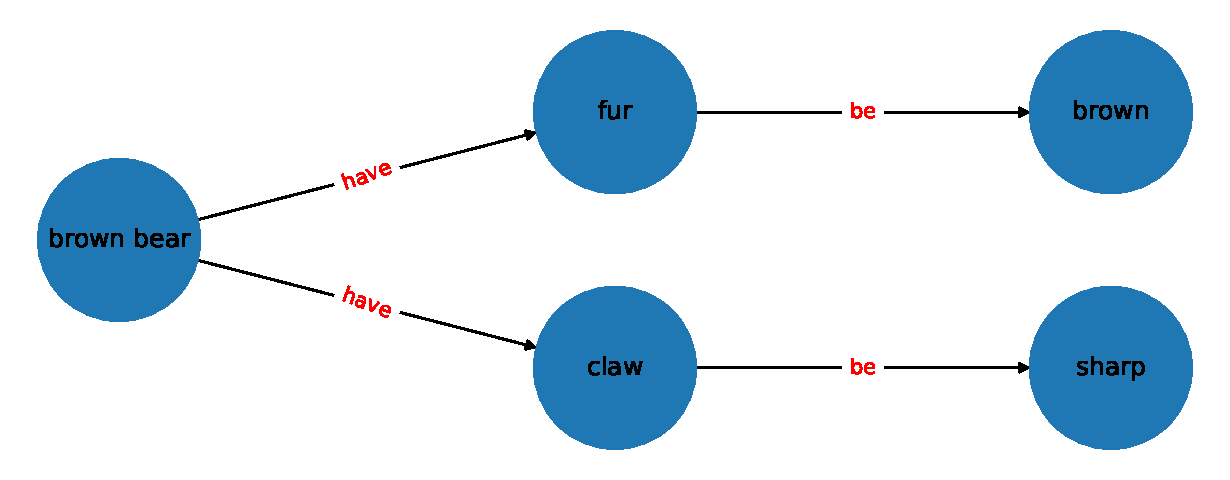
\includegraphics[width=\textwidth]{kn_example.pdf}
        \caption[Example of a knowledge graph]{The sentences result in five nodes (subject/object) and four edges (relations). The circles contain the objects/subjects and the arrows represent the relations.}
        \label{fig:graph_example}    
    \end{subfigure}
    \caption[Part of Speech tagging and knowledge graph]{The sentences are first broken down with the NLP pipeline of \textcite{honnibal_spacy_2020}. The extracted PoS tags and dependency tags are then used to construct the semantic triples In first case the first node is the normal subject (nsubj) combined witht the compound. The root verb of this subject is the relation and the direct object (dobj) of the verb is the object of the first semantic triple. For the last relation and node, the adjective modifier (amod) of the last node (fur) is used as object. In this case the relation is dependent on the PoS tag of the adjective modifier. In the last case the claws are a normal subject, but are treated as an object.}
    \label{fig:pos_pipeline}
\end{figure}

For PoS extracting we use the library of \textcite{honnibal_spacy_2020}.
This is a pretrained NLP model that can extract PoS tags and their dependencies.
We set up a rule-based system to extract data from the sentences.
In Figure \ref{fig:pos_pipeline} two (very simple) example sentences can be found that are processed using PoS tagging and dependency parsing with the pretrained pipelines of \textcite{honnibal_spacy_2020}.
We have the benefit that we already know the broad subject of every sentence, as each sentence corresponds to the queries species.
This means that we can have the species as starting node, even when the subject is not the species itself, see Figure \ref{fig:PoS_example2}.
Most researches do not have this and also need to determine the subject of every sentence \autocite{hutchison_knowledge_2013} like we do in \ref{fig:PoS_example}.
By processing this in a rule-base system we expect to create a knowledge graph like shown in Figure \ref{fig:graph_example}.
\end{comment}


\subsection{Information Extraction Techniques} \label{par:keywords}
We use two different ways to extract the essential words from the description sentences.
(1) several different post hoc explanation techniques (see Section \ref{par:attribution}), and (2) a rule-based system of PoS in combination with dependency parsing (see Section \ref{par:PoS}). 
We use the \href{http://www.vision.caltech.edu/visipedia/CUB-200-2011.html}{Caltech-UCSD Birds 200 dataset} (CUB-200) from  \textcite{welinder_caltech-ucsd_2010} to compare the techniques.
The CUB-200 dataset is a dataset with 200 bird species from Northern America.
Each bird is represented by approximately 60 images, and each of these images is hand-annotated with traits that are seen\footnote{Images are annotated with a certainty of the trait being present, we only use the traits that have the highest certainty in the image.}.

Before extracting keywords, we first match every sentence from our dataset against a bird glossary from \href{https://en.wikipedia.org/wiki/Glossary_of_bird_terms}{Wikipedia/Glossary/Birds}.
Matching sentences against the glossary allows us to create a similarity matrix per part instead of per bird (see Figure \ref{fig:similarity_workflow}).
%The CUB-200 dataset only contains visual traits, whereas our own bird dataset can also contain non-visual traits like behavioural traits or vocal traits.
From \href{https://en.wikipedia.org/wiki/Glossary_of_bird_terms}{Wikipedia/Glossary/Birds}, we extract 1,163 glossary terms related to birds\footnote{This list include the most common terms, but also similar terms. For example 'addled eggs ' has two glossary terms: 'wind eggs' and 'hypanema' that mean the same. We append all three term to the glossary list.}.
%Matching our own textual data against the bird glossary will also remove sentences that are incorrectly classified by our classifier and also saves computing power as we can first select the bird, then select a trait and finally match the results against the CUB-200 dataset (see Figure \ref{fig:similarity_workflow}).

\begin{figure} [htbp]
    \centering
    %\hspace{-2cm}
    %\hspace{-2cm}
    %\textbf{Similarity Matrix}
    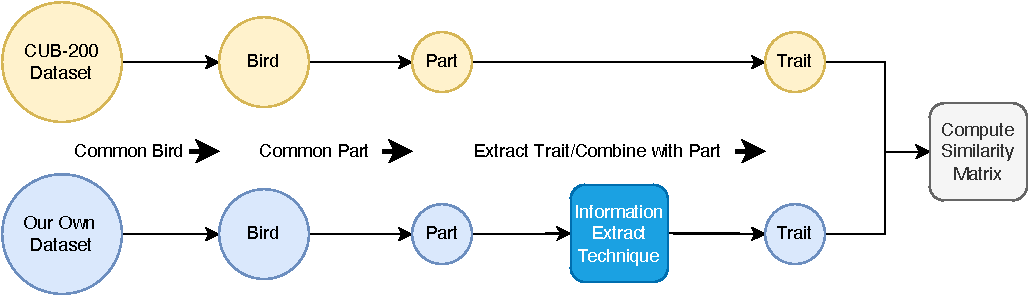
\includegraphics[width=1\textwidth]{figures/Similarity_workflow.pdf}
    \caption[Similarity Workflow]{The workflow to compare the datasets. We first select a common bird. Secondly we select a common part. With out own dataset we use an information extraction technique (attribution or PoS) to extract a adjective. The part and the adjective are combined, and the similarity against the CUB-200 dataset is calculated.}
    \label{fig:similarity_workflow}
\end{figure}

\begin{figure} [htbp]
    \centering
    %\hspace{-2cm}
    \hspace{-3cm}
    %\textbf{Similarity Matrix}
    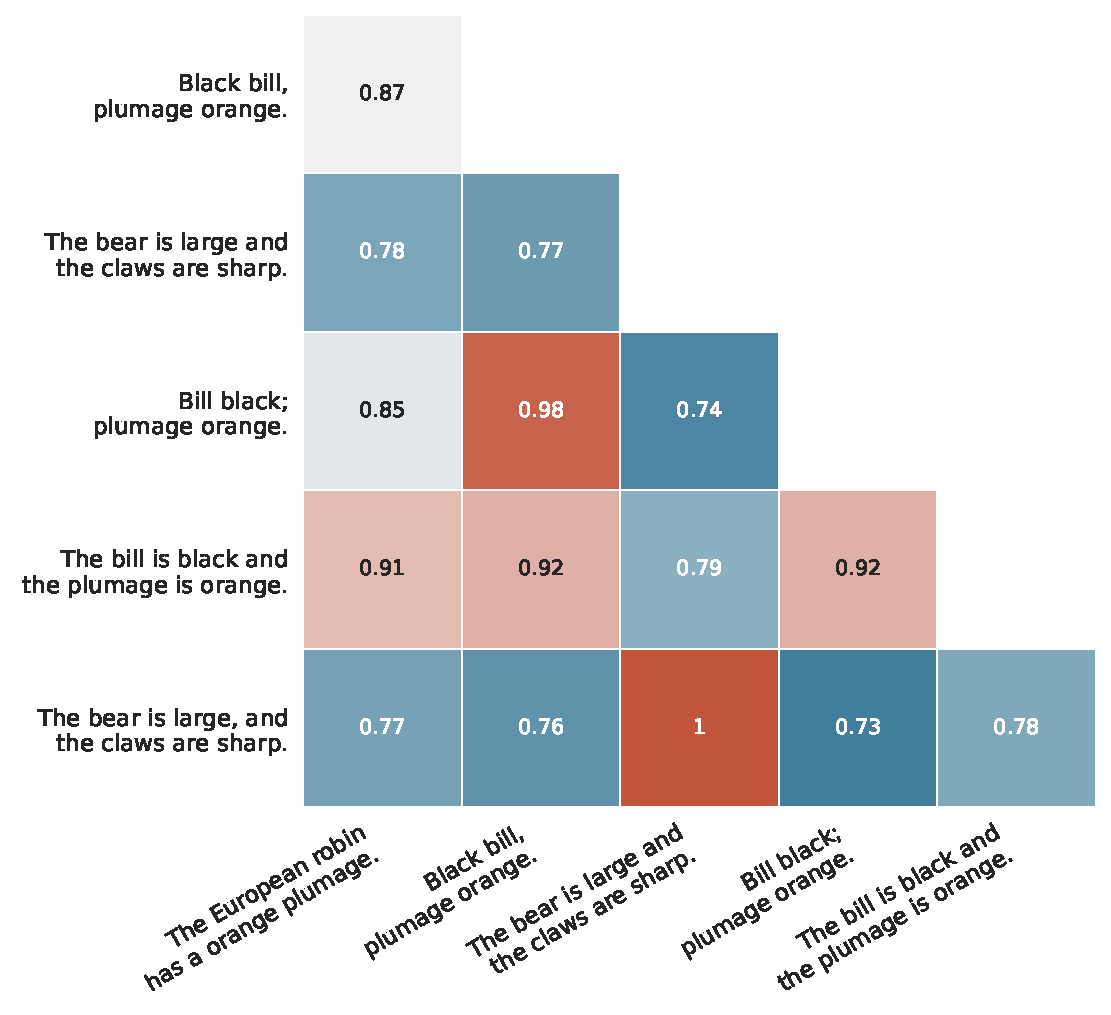
\includegraphics[width=0.8\textwidth]{similarity_matrix.pdf}
    \caption[Example of sentence similarity]{An example for the calculation of sentence similarity. 
    In this case reconstructed text chunks from the CUB-200 dataset are shown on the y-axis and reconstructed text chunks from scraped data is shown on the x-axis. In this case 'Bill colour yellow', and 'Bill yellow' is almost the same, hence the high similarity score of 0.91. Note that the matrix does not necessarily have to have equal rows and columns.}
    \label{fig:similarity_matrix}
\end{figure}



To compute the text similarity, we use an untrained version of distillBERT and compute the cosine similarity between the two outputs.
We tokenise each sentence and push it through the distilled version of BERT.
We sum the last hidden state along the first axis for each sentence, resulting in a matrix where the hidden state is summed for each token:
\begin{equation}
     \sum\nolimits_{j}^{} x_{ij} 
\end{equation}
Where~$i$ is 768 (the vector representation of a token) and~$j$ is the number of tokens. 
After this, we simply compute the cosine similarity of each text chunk against all the text chunks of the CUB-200 dataset:
\begin{equation}
\cos ({\bf A},{\bf B})= {{\bf A} {\bf B} \over \|{\bf A}\| \|{\bf B}\|} = \frac{ \sum_{i=1}^{n}{{\bf A}_i{\bf B}_i} }{ \sqrt{\sum_{i=1}^{n}{({\bf A}_i)^2}} \sqrt{\sum_{i=1}^{n}{({\bf B}_i)^2}} }
\end{equation} \label{eq:cosine_sim}
Where~$A$ is the vector of text chunk 1 and~$B$ the vector of text chunk 2. 
In Figure \ref{fig:similarity_matrix}, an example of a comparison of a few fictional text chunks can be found. 
Finally, we assess which technique delivers the best performance and select this for the test dataset.

For each unique bird, part and technique combination of the CUB-200 data and the data from the internet, we compute a similarity matrix.
We extract the highest value of each unique combination, resulting in a large array of similarity values per attribution.
The harmonic mean is computed to get the best attribution method:
\begin{equation}
    H = \frac{n}{\sum\limits_{i=1}^n \frac1{x_i}}
\end{equation}
Where~$H$ is the harmonic mean,~$n$ is the number of samples, and~$x$ is the similarity value. 

\subsubsection{Post Hoc Attribution Techniques} \label{par:attribution}
We try several posthoc explanation techniques to retrieve keywords from the description data\footnote{We do not use jittering techniques as this makes no sense in the case of text data, which results in fixed values when tokenised.}. 
We implement all techniques with the Captum library from \textcite{kokhlikyan_captum_2020}.
\begin{itemize}
    \item Layer Integrated Gradients (LIG), based on the paper of \textcite{sundararajan_axiomatic_2017}. We use LIG with 20 steps and with 100 steps.
    \item Occlusions, based on the paper of \textcite{fleet_visualizing_2014}. Although this is originally used to explain CNNs, it can also explain NLP models. We use two different versions of occlusion, (1) with a window and stride of both 1. (2) a window of 3\footnote{The windows is 1-dimensional in this case as the input vector is a tensor of the tokenised text.} and a stride of 2. In both cases, the word(s) will be replaced with a tensor of zeros to check the prediction changes of the model. 
    \item Shapley Value Sampling (SVS), based on the papers of \textcite{castro_polynomial_2009, strumbelj_efficient_2010}. We use the Captum default of 25 samples.
    \item Layer Activation (LA), which simple computes the activation of the internal BERT embeddings for the inputs.
    \item Layer Gradient X Activation (LGXA), which is the element-wise multiplication of the gradients and the layers activation for a giver target with respect to the layer.
\end{itemize}

We train a classification model on a subset of the BOW dataset.
We ensure that all the birds of the CUB-200 dataset are present in the birds presented to the model.
We random sample additional birds from the BOW dataset, so the CUB birds make up about 10\% of the total data and resulting in 2,000 birds, but birds with a high amount of HTML pages have priority during the sampling.
This way, we make sure birds with a decent number of descriptions are used in the training phase.
We use the web crawler with the trained binary classifier for descriptions to enrich the BOW dataset with sentences from the internet.
We do not split the model into train and test data, as evaluating with a test set has no use.
We use the same hyperparameters and architecture as we did for training the binary classification model (see Section \ref{par:Architecture}).
We only change the last linear output layer to match the number of species used during training.
After the model has been trained, we compute the attribution value for every word per sentence with the aforementioned techniques.

\subsubsection{Part-of-Speech \& Dependency Parsing} \label{par:PoS}
A \textit{knowledge graph} is a graph that contains interlinked descriptions of traits; the information has a formal structure that allows both humans and computers to process the data unambiguously \autocite{petkova_crafting_2020}.
If we apply this to species descriptions, we would expect to end up with a single graph per species containing descriptive information about that species semantically.
These graphs can also be linked if species share common traits.
Creating a knowledge graph of the sentence data will result in a clean database.
This database will only contain subjects, relations and objects, also known as semantic triples. 
We use the subject, relation and object to create a single text span to tokenise.

\begin{figure} [htpb]
    \centering
    \begin{subfigure}[b]{1.0\textwidth}
        \centering
        %\vspace{0cm}
        \includesvg[inkscapelatex=false, width=\textwidth]{PoS_example.svg}
        \caption[Example of part of speech tagging (1)]{An example of part of speech and dependency parsing for the sentence "The Brown bear has brown fur.".}
        \label{fig:PoS_example}
    \end{subfigure}
    \vfill
    \centering
    \begin{subfigure}[b]{1.0\textwidth}
        \centering
        %\vspace{0cm}
        \includesvg[inkscapelatex=false, width=0.6\textwidth]{PoS_example2.svg}
        \caption[Example of part of speech tagging (2)]{An example of part of speech and dependency parsing for the sentence "The claws are sharp.".}
        \label{fig:PoS_example2}
    \end{subfigure}
    \vfill
    \begin{subfigure}[b]{1.0\textwidth}
        \centering
        %\vspace{-2cm}
        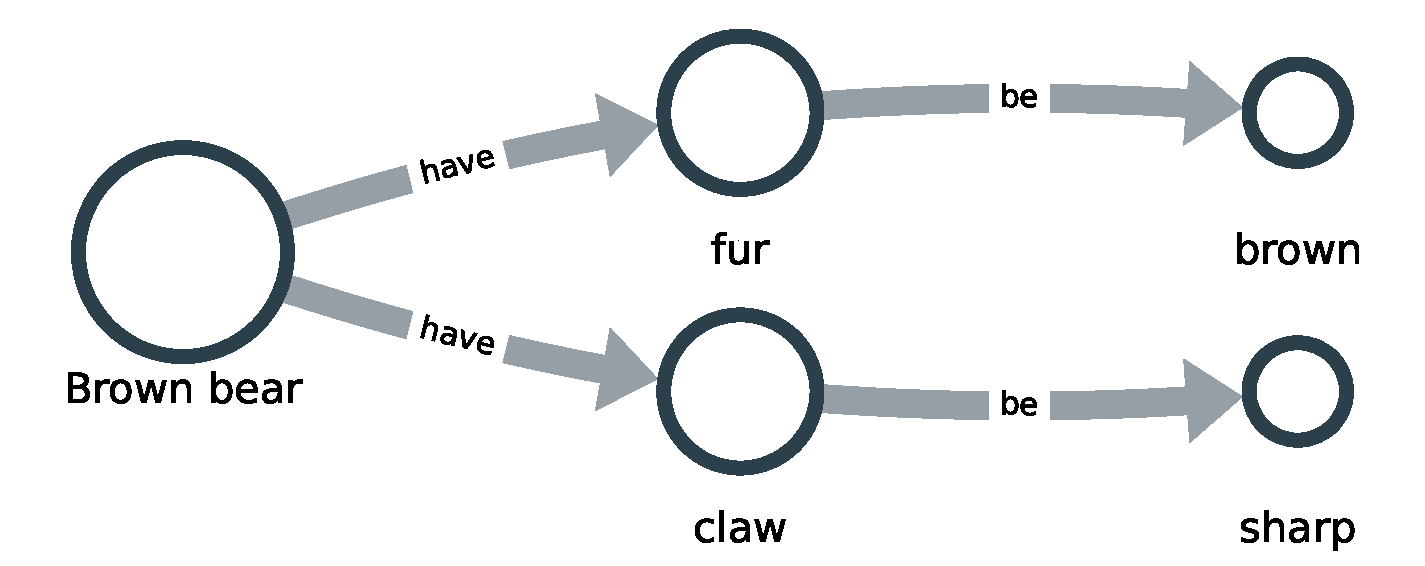
\includegraphics[width=0.65\textwidth]{kn_example_v2.pdf}
        \caption[Example of a knowledge graph]{A knowledge graph example. The circles contain the objects/subjects and the arrows represent the relations.}
        \label{fig:graph_example}    
    \end{subfigure}
    \caption[Part of Speech tagging and dependency parsing]{An example of part-of-speech tagging and dependency parsing to extract semantic triples for the creation of a knowledge graph. The arrows indicate the dependency tags and the abbreviations below the sentence contain the PoS tags. The sentences result in five nodes (subject/object) and four edges (relation). }
    \label{fig:pos_pipeline}
\end{figure}

We use PoS tagging and dependency parsing to create a clean knowledge graph.
For PoS extracting, we use the library of \textcite{honnibal_spacy_2020}; their pre-trained NLP model can extract PoS tags and the dependencies.
We set up a rule-based system to extract data from the sentences.
In Figure \ref{fig:pos_pipeline}, two example sentences can be found that are processed using PoS tagging and dependency parsing with the pre-trained pipelines of \textcite{honnibal_spacy_2020}.
We benefit from knowing the broad subject of every sentence, which is the species.
Most researchers do not have this and need to determine the subject of every sentence if they want to link all data \autocite{hutchison_knowledge_2013}, as we do in Figure \ref{fig:PoS_example}.
We know that every sentence describes the queried species; we can have the species as starting node, even when the subject is not the species itself, see Figures \ref{fig:PoS_example2} and \ref{fig:graph_example}.
By processing this in a rule-based system, we create a knowledge graph like Figure \ref{fig:graph_example}.

\subsubsection{Knowledge Graph Creation}
We use PoS in combination with dependency parsing to extract essential adjectives/trait combinations to create semantic triples.
This has proven to give the best results (See Section \ref{par:results_keywords} and especially Figure \ref{fig:hmean_violin}).
%We use the the technique with the highest harmonic mean to create a database from description sentences.
%We use this technique to extract the most important word/trait combinations to create a database.
The methods for extracting useful plant term is almost the same as for birds.
We first match every sentence against \href{https://en.wikipedia.org/wiki/Glossary_of_plant_morphology}{Wikipedia/Glossary/Plants},
Allowing us to remove irrelevant sentences that accidentally slipped through the classifier.
In Figure \ref{fig:glossary}, a small example is shown of how we match sentences against the glossary containing expert words.
\begin{figure} [htpb]
    \centering
    %\hspace{-2cm}
    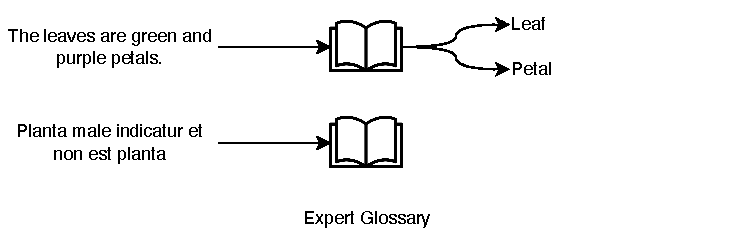
\includegraphics[width=0.8\textwidth]{figures/glossary_workflow.pdf}
    \caption[Expert Glossary Example]{An example how each sentences is matched against a glossary containing expert words. This way, misclassified sentences can be filtered out and irrelevant description can be dropped.}
    \label{fig:glossary}
\end{figure}


\begin{comment}
\begin{figure} [htpb]
    \centering
    %\vspace{-2cm}
    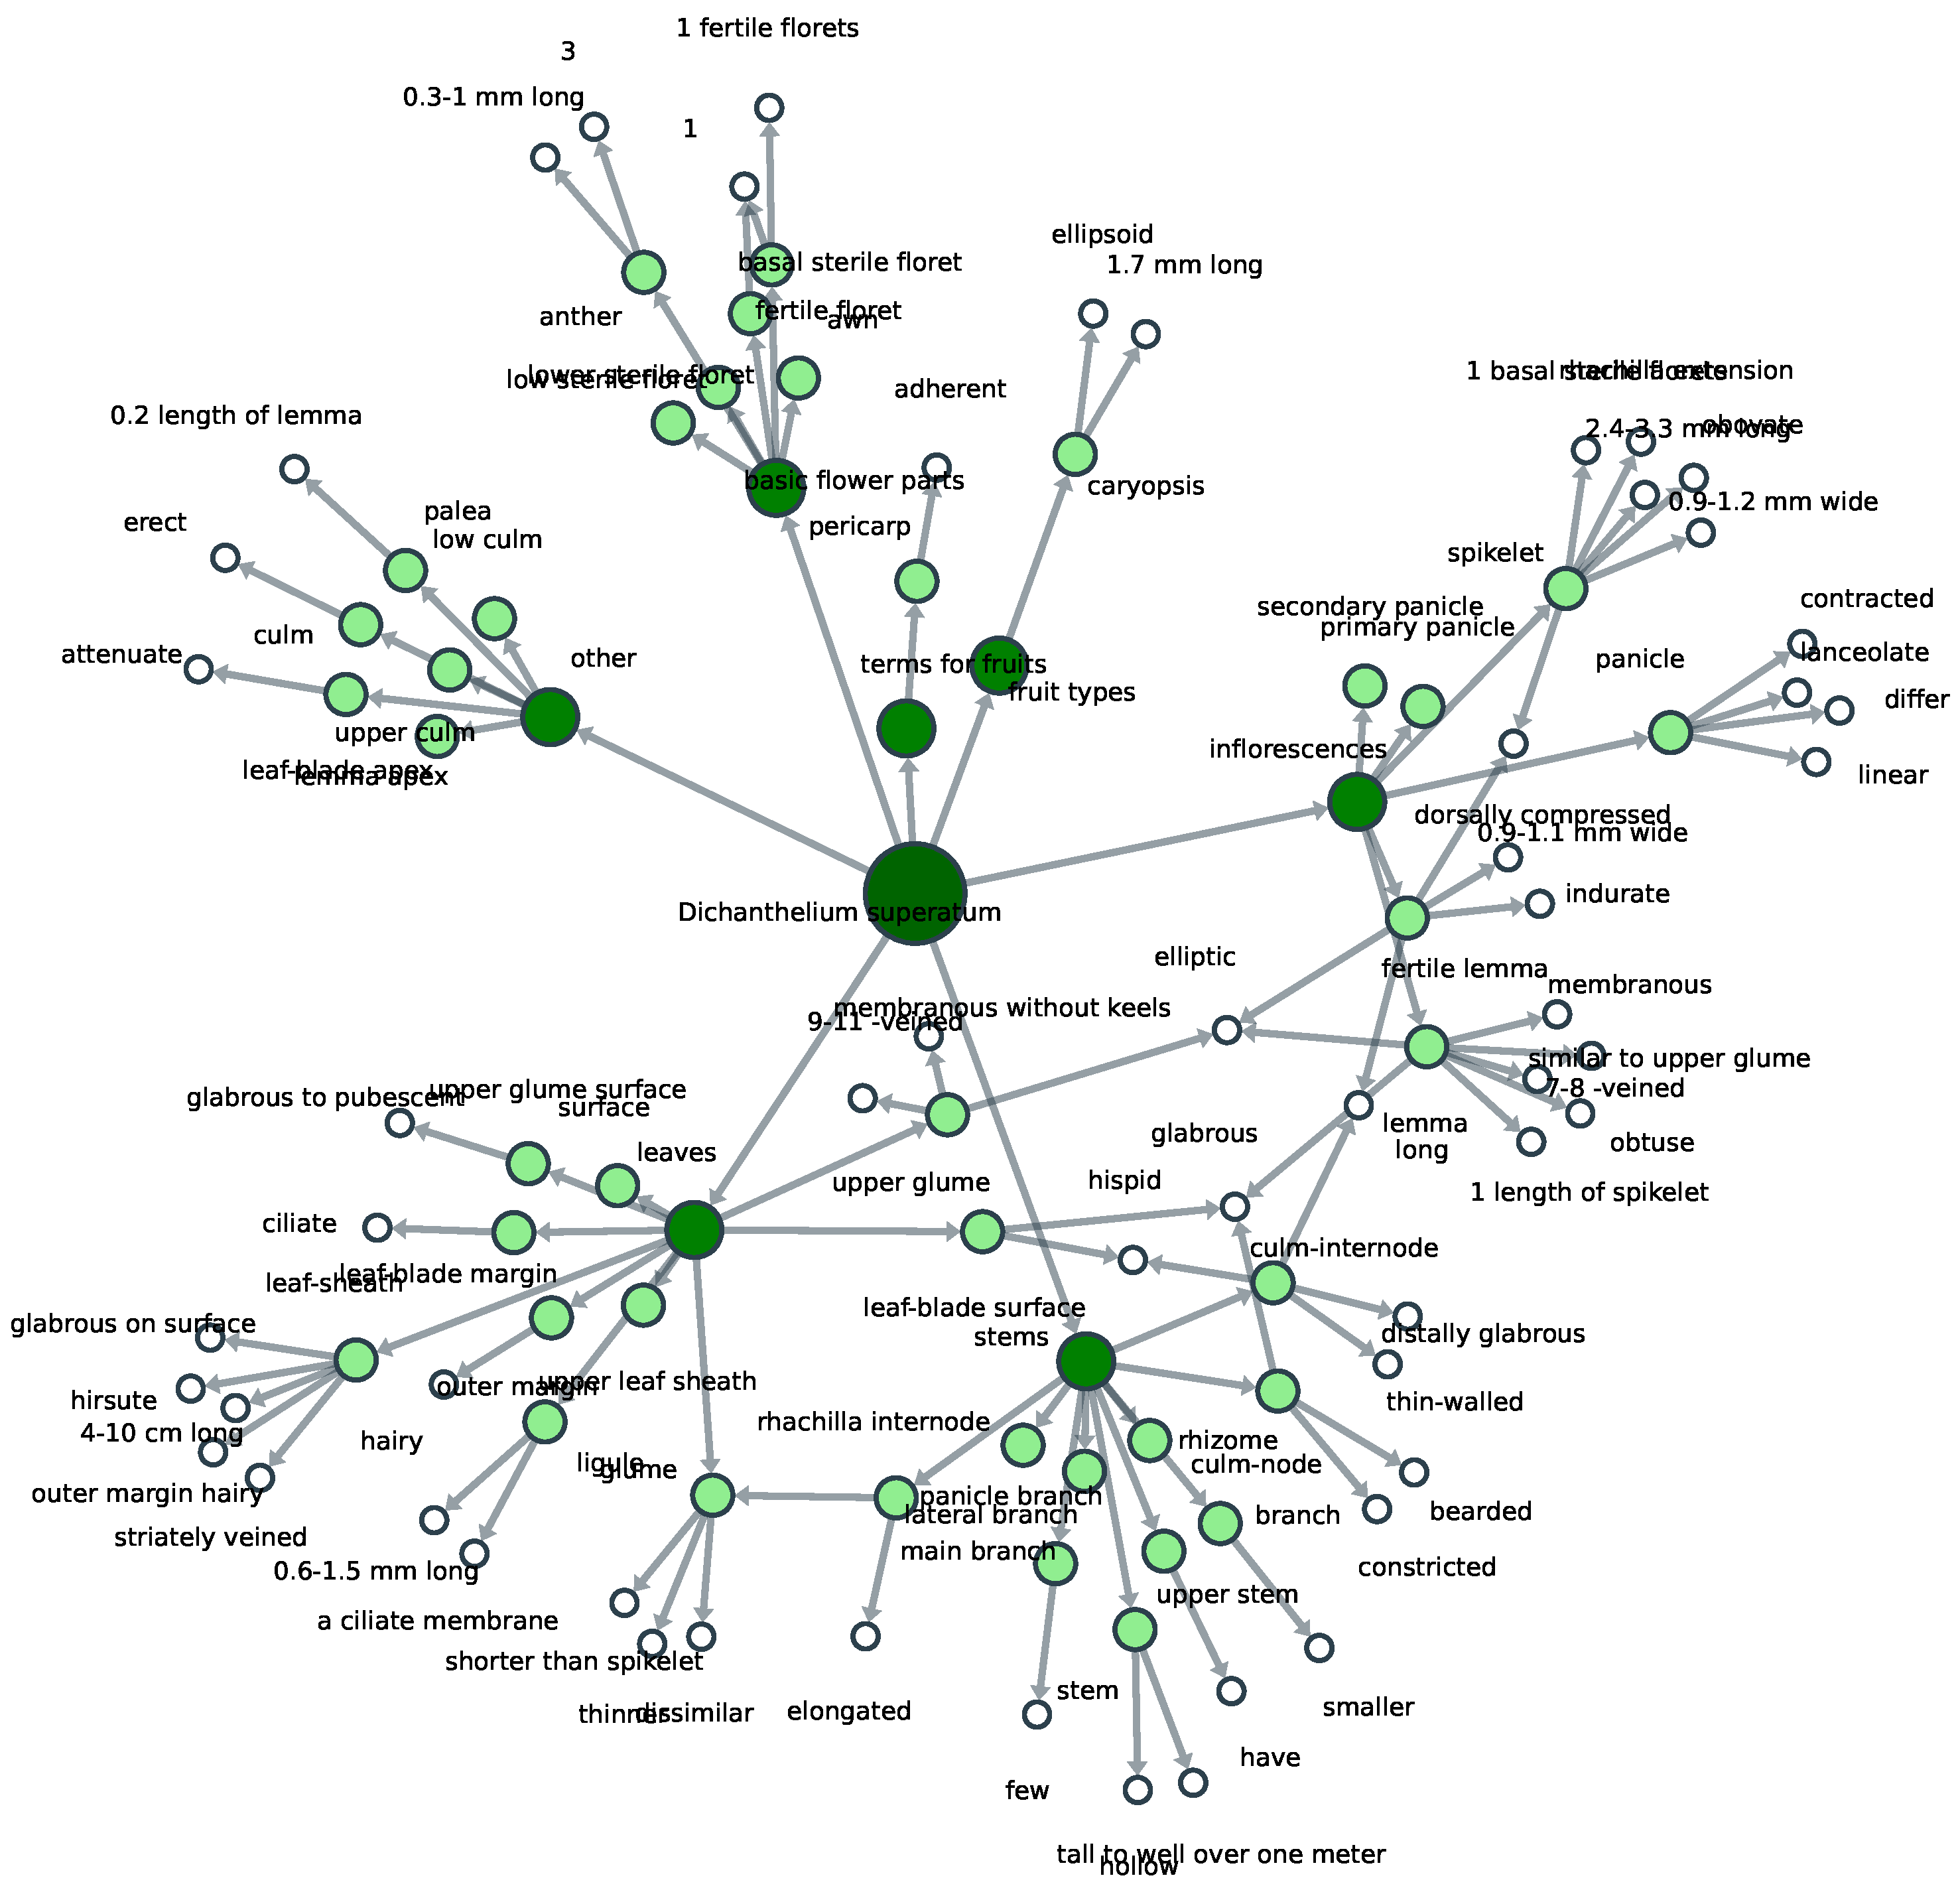
\includegraphics[width=\textwidth]{figures/kngraph.pdf}
    \caption[Example of automatic information extraction]{An example of the information extracted for a single species from the PoWO dataset. The center node (dark green) is the starting node. The green branches represent main parts of the plant (found in the glossary). The light green branches represent traits that are both found in the glossary and the sentence. Finally, the white ending node represent information (adjectives, appositional modifiers etc.) of the found trait. Note that the relations (edges/arrows: e.g. 'have', 'located at') are not shown plotted in this figure. For this example 35 sentences are used.}
    \label{fig:kngraph}
\end{figure}
\end{comment}

We use a plant species as a starting node.
From every sentence, nouns are checked against this glossary.
If a noun exists within the glossary, a node from the species $has\_main\_part$ to the header of the glossary and from the header to noun $has\_sub\_part$ is created.
However, because appending the noun to the knowledge graph, we first construct possible compound nouns.
This allows us to distinguish between, e.g. sexes (male/female) or locations (lower/upper).
Finally, we extract the adjectives and possible relations between the noun and adjectives.
During the process, we lemmatise all nouns and adjectives as much as possible, reducing the variation in the database and increasing the probability that species have shared traits/nodes.

We use a simple relation like $is$ or $has$ in most cases if the sentence does not contain any verbs or verbal modifiers.
In some cases, the verb of the sentences will result in the relation (edge), e.g. $elongated\_below$.
%In Figure \ref{fig:kngraph} a small example of information extraction from sentences of a single plant species (Dichanthelium superatum) can be found.
By applying this technique to all data, species have shared parts and even traits.
We hypothesise that an NLP model for inferring species based on the textual description will give better results.
It will become more challenging for a classifier to learn the unique vector representation because sentences are less likely to be unique for a single species.
In Figure \ref{fig:kngraph_unweighted}, a small example of a single species can be found.
\begin{figure} [htpb]
    \centering
    %\vspace{-2cm}
    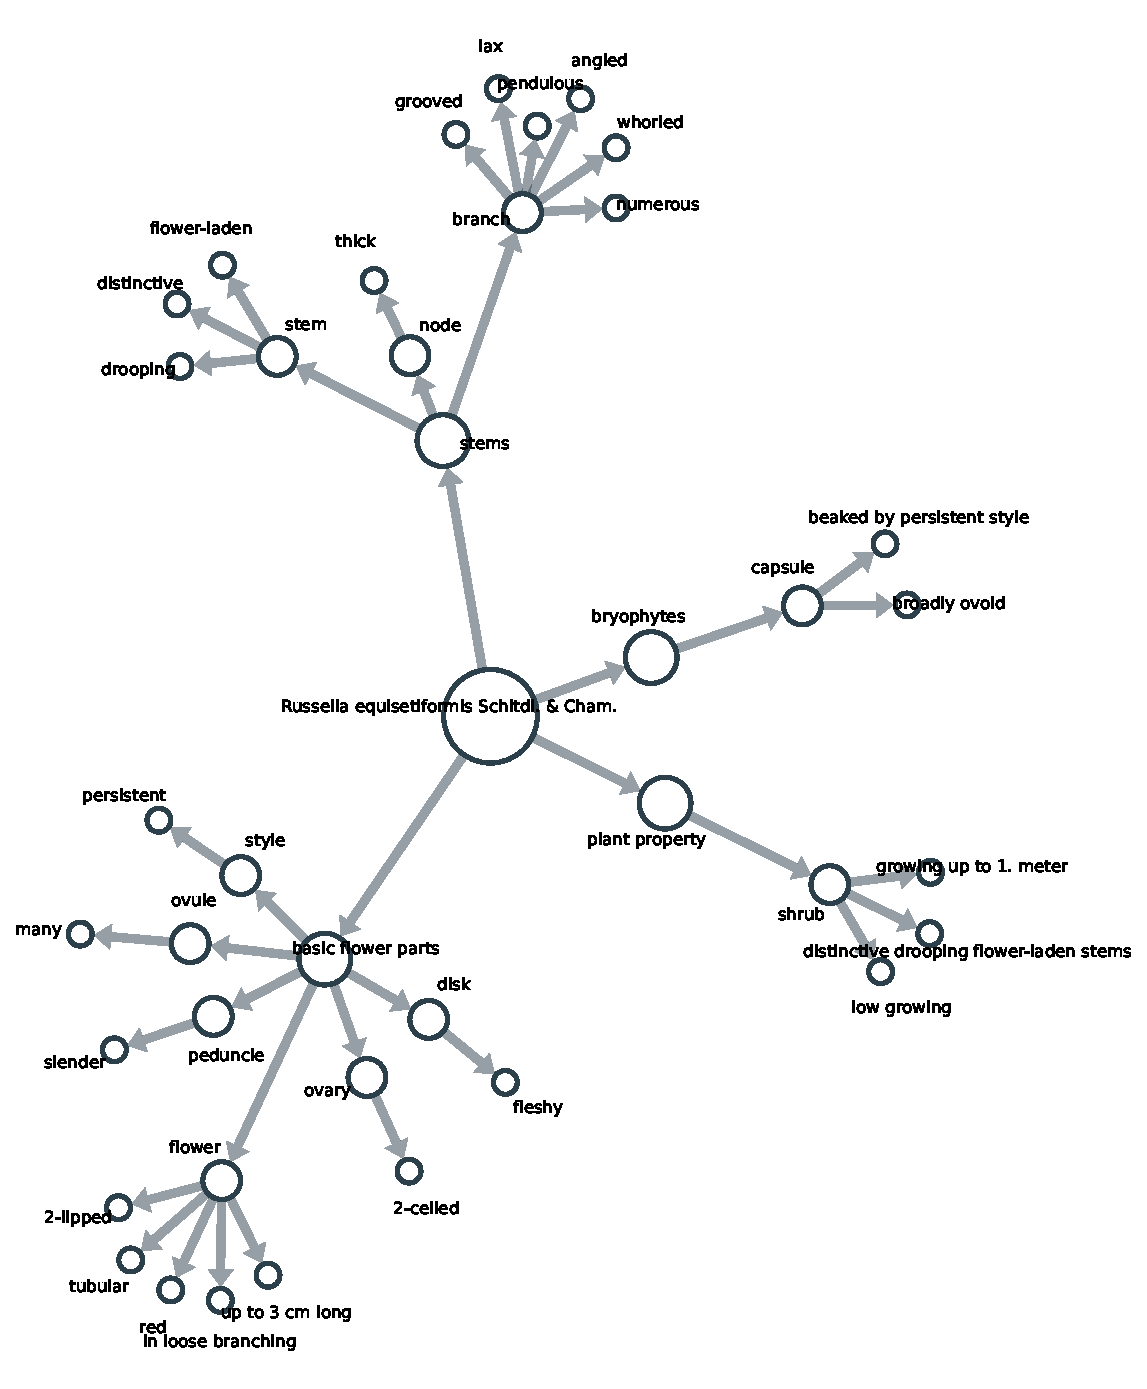
\includegraphics[width=\textwidth]{figures/kngraph_unweighted.pdf}
    \caption[Example of an unweighted knowledge graph]{An example of the information extracted for a single species we entered into the web crawler. Note that the relations are not shown plotted in this figure. For aesthetic reasons we only used the first 20 sentences for the graph.}
    \label{fig:kngraph_unweighted}
\end{figure}


\subsection{Evaluation Species Prediction} \label{par:species_prediction}
We cannot use a classic train/test split approach to train and validate the model.
If we leave certain species out of the training fase, the model cannot learn their distinctive traits.
If we leave out random parts of each species, some crucial information for that species might be lost.
To validate if the model learn anything (i.e. the prediction values are better than a random classifier) we use three separate datasets.
The PoWo dataset is used as training data and the Llifle and AgroForesty datasets are jointly used as testing data.
We first find plants species that are present in both sets with a simple intersection.
%Next we create semantic triples for every species and reconstruct every every semantic triple into a sentence.


\subsubsection{Data Preparation \& Training} \label{par:pos_training}
Section \ref{par:results_keywords} and especially Figure \ref{fig:hmean_violin}, show that PoS in combination with dependency parsing is the most promising technique to extract useful species descriptions from sentences.
We cannot directly use the graphs in a NLP model to predict species.
Graphs are complex, can a variable size and have no fixed forms, whereas text (which can also be represented as a graph) is relatively simple and is ordered to some extent \autocite{sanchez-lengeling_gentle_2021}. 
For simplicity, in this thesis we prepare the semantic triples for species prediction by creation single text span out of them.
Each text span exists of a start node, relation and end node.
The text span is finalised with a punctuation and is capitalised.
For Example, the nodes and relation $rhachilla\_internode$, $elongated\_below$ and $floret$ will be reconstructed to "Rhachilla internode elongated below floret.".
This allows us to tokenise the text span and push it trough a BERT model with a linear classifier on top of it.
In Figure \ref{fig:kngraph_unweighted} a small example of a knowledge graph can be found.
%We freeze all the internal parameters of BERT and train only the linear classifier.
%To see if the linear classifier learn anything we use the the PoWo dataset as training data and we use the Llifle and AgroForesty datasets and testing data.
We use the same architecture as in Figure \ref{fig:model_architecture} and only train the linear classifier of the model and keep the parameters of distillBERT frozen.
The same hyperparameters found by \textcite{sun_how_2020} are used and the model is trained for 500 epochs.

\subsubsection{Calculation Probabilities}
The model will output a prediction value per species per created text span.
We use the negative log values\footnote{These are the actual output values of the model. We use \(e^{x}\), where~$x$ is the output, to convert the output back to probabilities in normal training. }. to evaluate if the model has learned anything. 
We sum the negative log values to combine the sentences per species. 
A small example can be found in Figure \ref{fig:species_probabilities}.
Figure \ref{fig:probs_nonstacked} contains the negative log values and prediction value per sentence for a single species, and Figure \ref{fig:probs_stacked} contains the summed negative log values and corresponding prediction.
In this example, the test set for the species contains 54 sentences that we created from the semantic triples.
The top Figure of Figure \ref{fig:probs_nonstacked} shows the model deemed seven text spans (probability > 0.1) distinctive enough.
The lower Figure Figure \ref{fig:probs_nonstacked} with the negative log probabilities shows that none of the text sentences has a very low log value for the correct species.
The datasets describe similar traits for the same species, and the model does a good job classifying the species.

Figure \ref{fig:probs_stacked} shows the combined probabilities and shows the summed log values.
In this Figure, it is visible that the more sentences are used, the higher the prediction certainty of the model is.
%In this Figure the prediction values of the incorrect species become more clear in the Figure with the summed log values.
The top Figure of Figure \ref{fig:probs_stacked} shows that the model has found the correct species around the tenth sentence.
We calculate the probabilities from the summed log values using a softmax function to squeeze all values between 0 and 1:
\begin{equation} \label{eq:softmax}
    \sigma(\mathbf{z})_i = \frac{e^{z_i}}{\sum_{j=1}^K e^{z_j}}
\end{equation}
Where~$z$ are the log values and~$\sigma$ is an output vector with probabilities with a sum of exactly 1.00.
Note that the order of the sentences is randomised, and the order of the sentences does influence the number of sentences it takes to find the correct species.
We could sort the sentence based on their prediction values of \ref{fig:probs_nonstacked} to decrease the number of sentences that are needed to obtain 100\% certainty.
However, as we only look at the final result, the order no longer matters.

\begin{figure} [htpb]
     \centering
     \begin{subfigure}[b]{1\textwidth}
         \centering
         %\hspace{-0.5cm}
         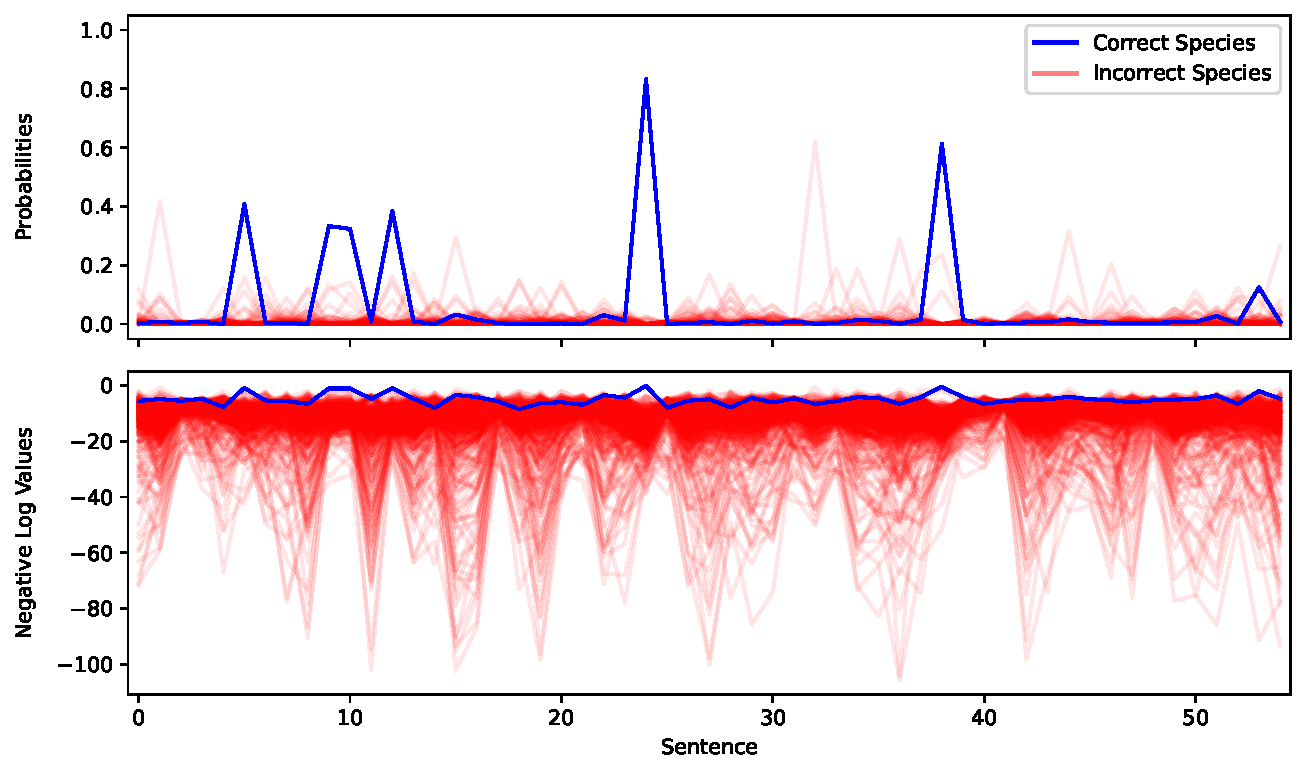
\includegraphics[width=\textwidth]{figures/probs_nonstacked.pdf}
         \caption{The prediction probabilities and the negative log values.}
         \label{fig:probs_nonstacked}
     \end{subfigure}
     \vfill
     \begin{subfigure}[b]{1\textwidth}
         \centering
         %\hspace{-0.5cm}
         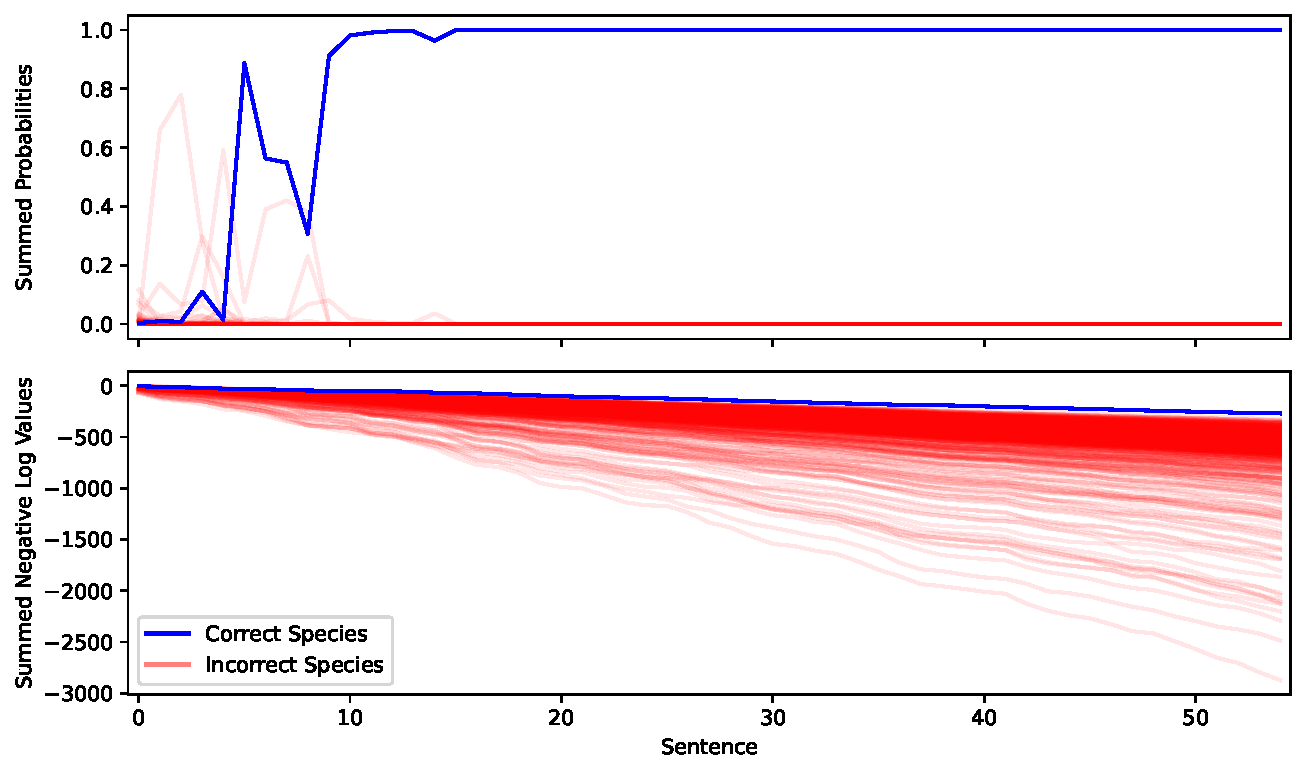
\includegraphics[width=\textwidth]{figures/probs_stacked.pdf}
         \caption{The prediction probabilities based on the summed values and the summed negative log values.}
         \label{fig:probs_stacked}
     \end{subfigure}
     \caption[Species Prediction Probabilities]{An example the prediction of a species. The prediction is done per sentence, the result of the model is a negative log value that can be converted into a probability. By summing the negative log values we can get a probability for the combined sentences. In this example the model reaches a prediction value of 1.0 with the first 12 sentences.}
     \label{fig:species_probabilities}
\end{figure}


We take the final summed negative log  value of the combined sentences for each test species to see if the model learned anything.
We summed negative log values of the correct prediction against the average summed negative log values of the incorrect prediction.
As the data will be distributed non normally (-inf to 0) and the data are paired, we use a Wilcoxon Signed-Rank Test to test the paired samples against each other \autocite{wilcoxon_individual_1945}.
%We statistically test the correct prediction (one per species) against the incorrect predictions (number of test species minus one).
%As the data will be distributed non-normally (-inf to 0) and the data is paired  we use a Mann–Whitney U test \autocite{mann_test_1947} to see whether both distribution differ significantly from each other.
We will use an \(\alpha\) of 0.01 to determine if the model has learned anything. 


\subsection{Evaluation Information Extraction}
%We test our complete workflow against two different datasets. 
%(1) We test is against the Palm Trait dataset from \textcite{kissling_palmtraits_2019} and (2) we test our workflow against manually created species descriptions matrices.
%We use the Palm Trait dataset to automatically assess the results of our workflow and we use the manually created species description matrices and compare them manually against our workflow results.
We test our complete workflow against two different datasets. 
(1) We test is against the Palm Trait dataset from \textcite{kissling_palmtraits_2019} and (2) we test our workflow CUB-200 dataset from \textcite{welinder_caltech-ucsd_2010}.
We use both datasets to automatically assess the results of our workflow.


\subsubsection{Palm Trait Dataset comparison} \label{par:palmtrait_methods}
The Palm Trait dataset of \textcite{kissling_palmtraits_2019} contain over 2,500 palm plant (Arecaceae) traits. 
The Palm Trait dataset contain measurements, shape descriptions, colours descriptions and parts present.
The dataset describes the based parts of the palms, such as growth form, stems, armature, leaves and fruits.
Some parts are described using binary variables (e.g. StemErect = 1.0), other are described using words (e.g. FruitColor = Purple; Yellow) and most parts are described using integers (e.g. LeafNumber = 7, StemHeightMeter = 18).
We only use palm species that are complete within the Palm Trait database, leaving us with 248 species.
Each palm species is presented to the web crawler and we create a knowledge graph for each species.
\newline

\noindent
\textbf{Binary Class Variables.}
In case of binary variables we search for direct matches (e.g. 'erect' in the case of StemErect and 'armed' in case of StemArmed).
We use the normalised zero one loss \autocite{sammut_zero-one_2010} to calculate the accuracy of the workflow.
In some cases, using this loss, can result in biased accuracy.
For example in the case of StemArmed, we search for the term 'armed'. When this term is found, it results in a one and a zero otherwise. 
If most palms are not armed, the accuracy will be high.
\newline

\noindent
\textbf{Multi Class Variables.}
We search for direct hits of multi class variables.
This is the case for fruit colours (e.g. 'red') and fruit shapes (e.g. 'ovoid').
We first subset our knowledge graph, so it only contains information about the palm fruit. 
The knowledge graph is not subset any further.
We report the results with a confusion matrix and report the precision, recall, and F1-score.
\newline

\noindent
\textbf{Numeric Variables.}
In most cases, the Palm Trait dataset contains numeric variables.
We again take the appropriate subset of our knowledge graph.
Now, we search for the closest value in our knowledge graph subset.

\subsubsection{CUB-200 Dataset comparison}
To compare the results of our own dataset, we use the same approach as in Figure \ref{fig:similarity_workflow}.
We compare our dataset against the hand-annotated CUB-200 dataset.
We take a common bird and a common part, and push both description through a untrained DistillBert model to retrieve the vector embeddings.
Next, we compare both embeddings by computing the cosine similarity, and take the highest value from every similarity matrix:
\begin{equation}
    m=\max(0,  {X_i}_j  )
\end{equation}
Where $m$ is the maximum value and $X$ is the matrix per bird per part.
We sum all the maximum values:
\begin{equation}
     s=\sum_{1=i}^{n} m_i
\end{equation}
Where $s$ is the total similarity value for a bird, $m$ are the maximum values from the matrices and $n$ is the number of parts (between 0 and 15).
When the same part is not available in both datasets, we sum a zero.
For all birds this will results in a similarity value between 0.0\footnote{In this case not a single common part in present in both datasets.} and 15.0\footnote{In this case both datasets completely overlap with all parts and have 100\% similarity for all text samples.}.

As is makes no sense to compare these values, we rank the values for each bird in our dataset against the CUB dataset.
This ranking process will result in a heatmap with values between 1 (highest rank) and 200 (lowest rank) for every bird in our own dataset against the birds in the CUB dataset.
If every bird in our own dataset has a high similarity with the CUB dataset, it will result in a high ranking values.
We will match the average ranking value of our dataset against 200 times random sampling a value between 1 and 200.


\subsection{Information Importance}
We start by querying web pages that contain possible textual description using the web crawler.
We extract information from the sentences that are returned the same way we described in Section \ref{par:PoS} and prepare the data like we described in Section \ref{par:pos_training}.
This will result in a graph per species describing the species in a semantic way.
We again create text spans from node-edge-node relations and train a linear classifier NLP classifier on the data.
We use the same architecture as in Figure \ref{fig:model_architecture} and keep the batch size and learning rate the same.
We train the model for 1,000 epochs.


To calculate the relative importance of each node-edge-node, we push all the samples for a single species\footnote{We do not split the data into a train and test set and use all 229 species for training} through our trained classifier.
We calculate the negative log values for each sample.
After all values are calculated we use a softmax (Equation \ref{eq:softmax}) to compute the relative importance of all samples for a single species.
In Figure \ref{fig:kngraph_weighted} a small example can be found for a knowledge graph where the nodes have been colourised based on their importance.
We colourised based on the last node of a text span.
For example, the node $ovary$ is colourised based on the importance of the text span "Basic flower parts have ovary." and the node $up\_to\_3\_cm_\_long$ on "Flower measures up to 3 cm long."

Figure \ref{fig:kngraph_weighted} shows for the species 'Russelia equisetiformis Schltdl. \& Cham.' the most important nodes of a subset of 20 random sentences.
We hypothesise that branches that are deemed more important are more distinctive for 'Russelia equisetiformis Schltdl. \& Cham.'.
In this small example the facts that this species is a shrub growing up to 1 meter and that the flowers are 2-lipped could be distinctive as they both have a high importance compared to the other nodes.
As expected node-edge-node relations that are shared across many species, like the text span "Species has basic flower parts." have a relatively low importance and are thus distinctive. 


\begin{figure} [htpb]
    \centering
    %\vspace{-2cm}
    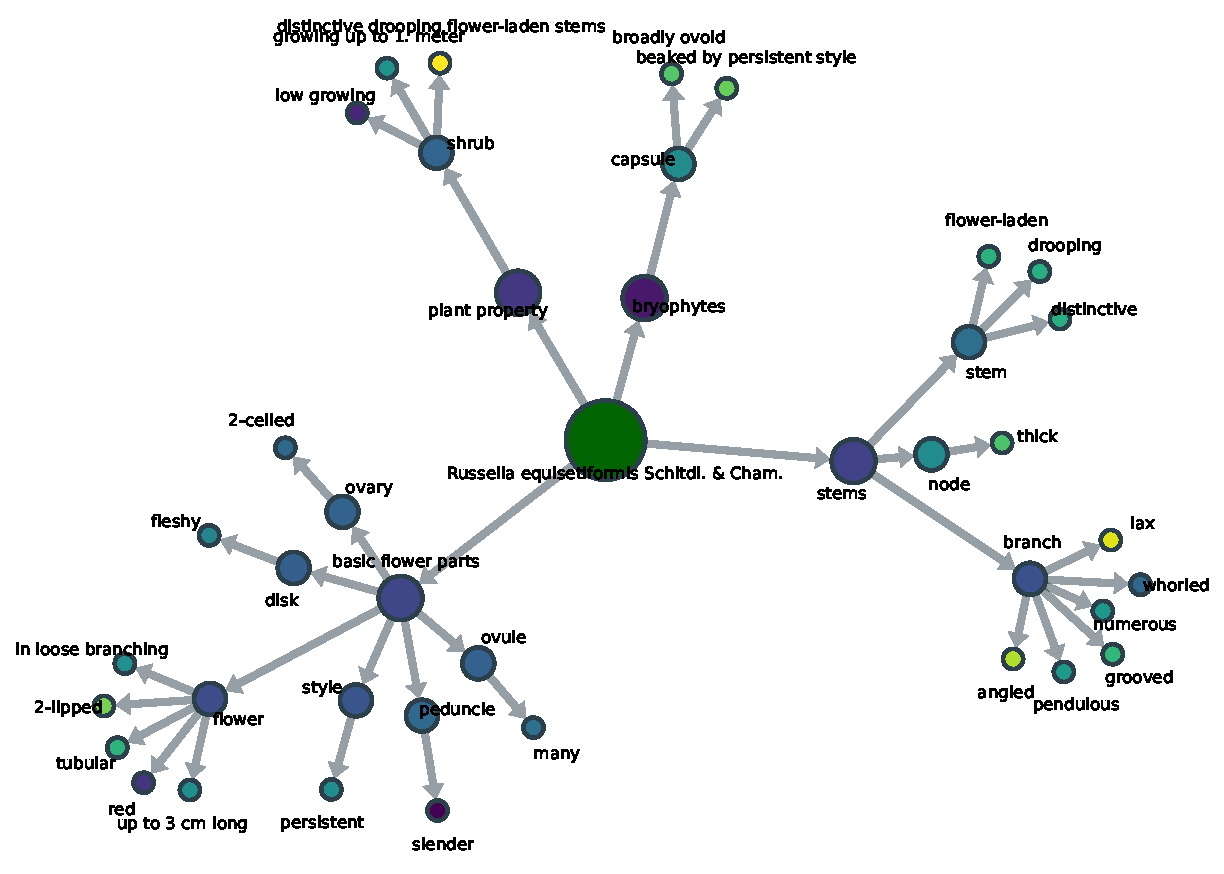
\includegraphics[width=\textwidth]{figures/kngraph_weighted.pdf}
    \caption[Example of an weighted knowledge graph]{The same knowledge graph as Figure \ref{fig:kngraph_unweighted}, only in this figure the nodes are colourised based on their importance. Yellow means a high importance value and deep blue means not important at all.}
    \label{fig:kngraph_weighted}
\end{figure}

\newpage
\section{Results} \label{par:results}
\markboth{Results}{Results}
\subsection{Species Descriptions}
\subsubsection{Description Classification Model} \label{par:results_binary_classifier}
Scraping the structured sources and using their paragraph titles resulted in 1,461,884 samples before splitting the sample into random text chunks.
1,105,576 samples correspond to label zero, and 356,308 correspond to label one.
%Each sample consists of a tuple, containing the label (0/1) and the text span.
Splitting the samples into text chunks resulted in 2,258,162 text chunks.
1,678,830 chunks have a label corresponding to something different (label 0) 579,332 chunks have a label corresponding to a description (label 1).
In Figure \ref{fig:text_length_distribution}, the text length distribution before and after splitting the original samples into random chunks can be found.
As shown from Figures \ref{fig:text_length_1}, \ref{fig:text_length_3}, \ref{fig:text_length_2}, and \ref{fig:text_length_4}, all distributions of the text lengths are left-skewed. 

\begin{figure} [htpb]
     \centering
     \begin{subfigure}[b]{0.49\textwidth}
         \centering
         %\hspace{-0.5cm}
         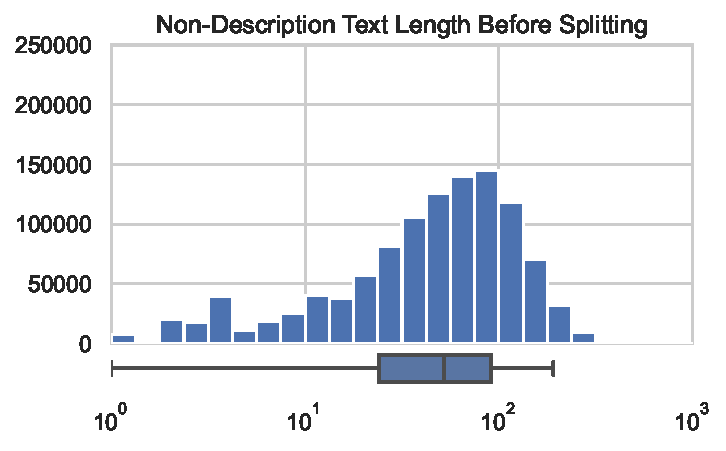
\includegraphics[width=\textwidth]{figures/histogram_text_length_1.pdf}
         \caption{The text length of non-description data before splitting.}
         \label{fig:text_length_1}
     \end{subfigure}
     \hfill
     \begin{subfigure}[b]{0.49\textwidth}
         \centering
         %\hspace{-0.5cm}
         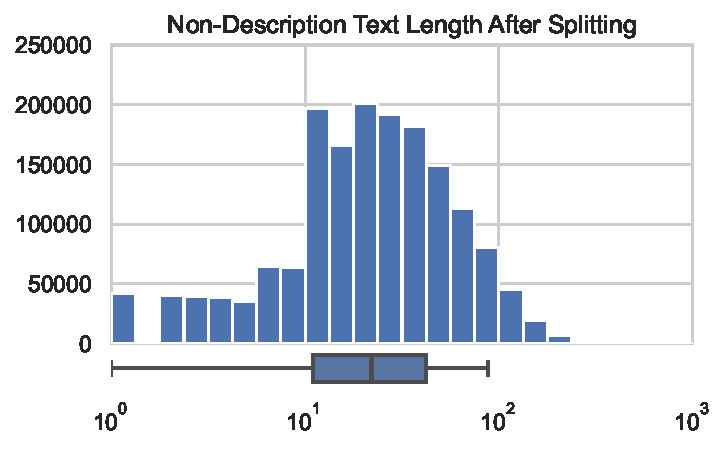
\includegraphics[width=\textwidth]{histogram_text_length_3.pdf}
         \caption{The text length of non-description data after splitting.}
         \label{fig:text_length_3}
     \end{subfigure}
     \vfill
     \begin{subfigure}[b]{0.49\textwidth}
         \centering
         %\hspace{-0.5cm}
         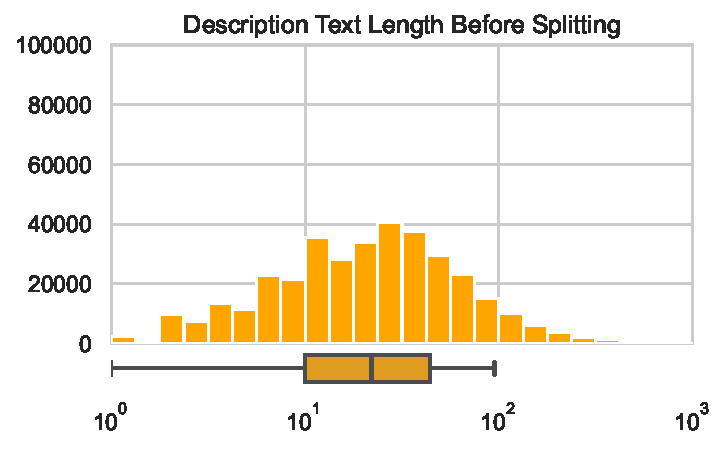
\includegraphics[width=\textwidth]{histogram_text_length_2.pdf}
         \caption{The text length of description data before splitting.}
         \label{fig:text_length_2}
     \end{subfigure}
     \hfill
     \begin{subfigure}[b]{0.49\textwidth}
         \centering
         %\hspace{-0.5cm}
         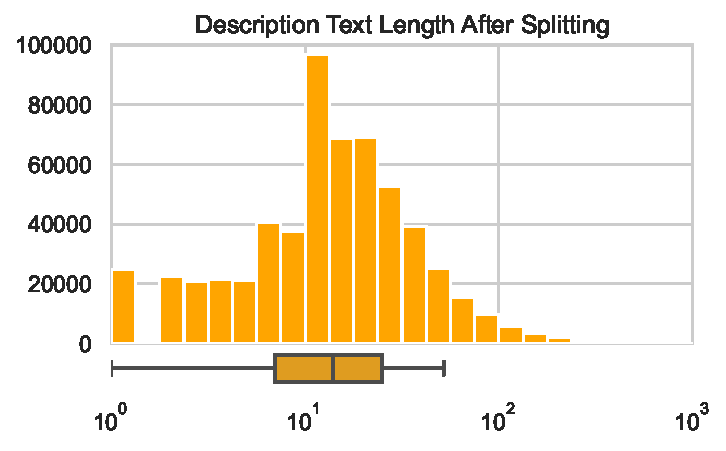
\includegraphics[width=\textwidth]{histogram_text_length_4.pdf}
         \caption{The text length of description data after splitting.}
         \label{fig:text_length_4}
     \end{subfigure}
    \caption[Text length distribution for training web crawler model]{The result of scraping structured sources to train  a binary classification model for descriptions classification. The text spans are randomly split into chunks between 10 words and their maximum length, with a maximum of 512 words to prevent truncation. Text spans with a length below 10 words are not split, resulting in some text lengths below 10. Note that outliers of the boxplots are not shown.}
    \label{fig:text_length_distribution}
\end{figure}


The model is evaluated on a held-out test set of 5\% and is evaluated on two held-out datasets, the \href{http://www.llifle.com/}{LLifle} and the \href{https://www.worldagroforestry.org/}{AgroForestry} dataset.
The summary performance metrics can be found in Table \ref{tab:precision_recall_metrics}.
The model reaches high precision, recall and F1-score for both the "Non-Description" and "Description" classes.
%These datasets are completely left out of the training/testing fase of the model.
%Together, these dataset contain 17,204 samples.
%771 text spans correspond to a description, and 16,433 text spans corresponds to something different.
%After the text has been cleaned and split into sentences there are 74,836 samples.
%There are 8,590 samples with a descriptions sentence and 66,246 samples that contain a sentence describing something %different.
%In Table \ref{tab:precision_recall_descriptionsmodel_external} the precision-recall summary for the external datasets can be found.
% Please add the following required packages to your document preamble:
% \usepackage{booktabs}
% Please add the following required packages to your document preamble:
% \usepackage{booktabs}
\begin{table}[htpb]
\centering
\caption[Precision-recall metrics test and two left out datasets]{The precision-recall metrics for the binary classification model tested on the test dataset and two external datasets (LLifle and AgroForestry).}
\label{tab:precision_recall_metrics}
\begin{tabular}{@{}lcccccccc@{}}
\cmidrule(l){2-9}
 & \multicolumn{2}{c}{\textbf{Precision}} & \multicolumn{2}{c}{\textbf{Recall}} & \multicolumn{2}{c}{\textbf{F1-score}} & \multicolumn{2}{c}{\textbf{Support}} \\ \cmidrule(l){2-9} 
                 & Test & Extern & Test & Extern & Test & Extern & Test    & Extern \\ \midrule
Other            & 0.98 & 0.96   & 0.99 & 0.96   & 0.99 & 0.97   & 167,955 & 64,639 \\
Description      & 0.97 & 0.83   & 0.95 & 0.77   & 0.96 & 0.83   & 57,864  & 10,197  \\ \midrule
Accuracy         &      &        &      &        & 0.98 & 0.95   & 225,819 & 74,836 \\
M Average        & 0.98 & 0.90   & 0.97 & 0.87   & 0.98 & 0.89   & 225,819 & 74,836 \\
W Average        & 0.98 & 0.95   & 0.98 & 0.95   & 0.98 & 0.95   & 225,819 & 74,836 \\ \bottomrule
\end{tabular}
\end{table}
As the classes are imbalanced in both cases, we evaluated the model with a precision-recall plot and not a receiver operator curve (ROC) figure, as precision-recall curves give a better overview of imbalanced datasets \autocite{saito_precision-recall_2015}.
The results of this plot can be found in Figure \ref{fig:precision-recall}, Figure \ref{fig:precision_recall_curve_test} contains the precision-recall plot for the test set, and Figure \ref{fig:precision_recall_curve_test_external} contains the precision-recall plot for the left out datasets.
\begin{figure} [htpb]
     \centering
     \begin{subfigure}[b]{0.48\textwidth}
         \centering
         %\hspace{-0.5cm}
         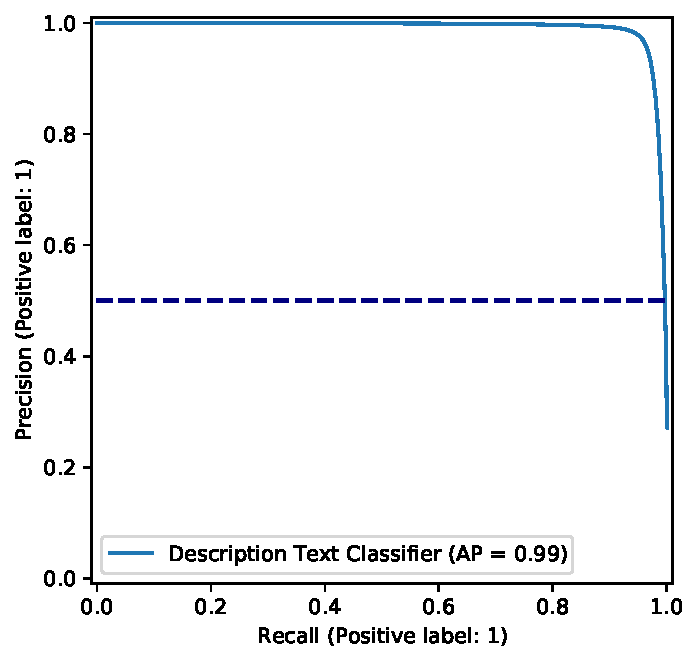
\includegraphics[width=\textwidth]{precision_recall_plot.pdf}
         \caption{The Precision-Recall curve for the test data.}
         \label{fig:precision_recall_curve_test}
     \end{subfigure}
     \hfill
     \begin{subfigure}[b]{0.48\textwidth}
         \centering
         %\hspace{-0.5cm}
         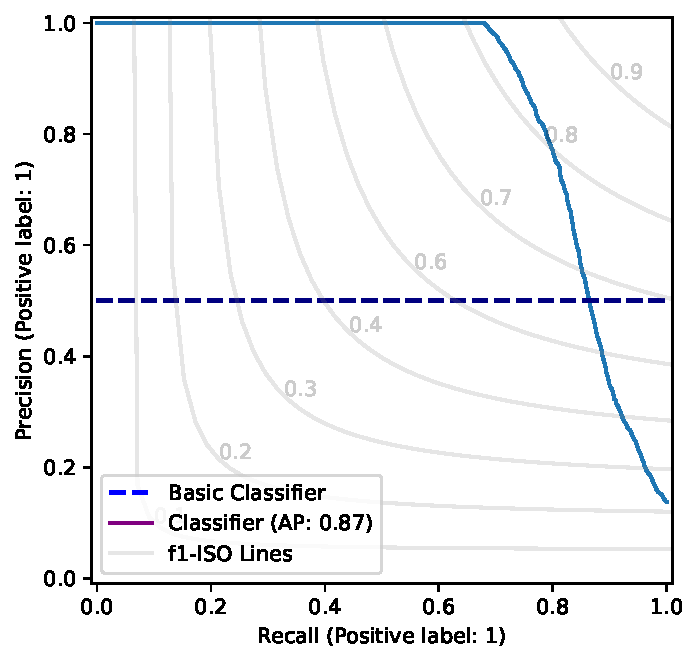
\includegraphics[width=\textwidth]{precision_recall_plot_extern.pdf}
         \caption{The Precision-Recall curve for the left out data.}
         \label{fig:precision_recall_curve_test_external}
     \end{subfigure}
     \caption[Precision recall curves for test and held-out datasets]{The precision-recall curve for the test dataset and the left out datasets. The model seems to perform reasonable in both cases. The the Average Precision (AP) reaches 99\% in the case of the test dataset and the AP reaches 87\% in the case of the held-out datasets. The area under the curve (AUC) reaches 99.49\% for the test set and 93.14\% for the held-out datasets.}
     \label{fig:precision-recall}
\end{figure}

In Figure \ref{fig:predictionvalues_external} the prediction values and the distribution the prediction values of the classifier for the two held-out datasets can be found.

%{The distribution of the two held-out datasets. In the first figure all the values are shown. In the second only values between 0.2 and 0.8 are shown as values below 0.2 and above 0.8 are always treated as correct. Note that the bars are stacked in the second figure, making the correctly classified and misclassified as high a the corresponding bars from the first figure. In both figures each bin has a width of 0.01.}

\begin{figure}[htpb]
 \centering
 %\hspace{-0.5cm}
 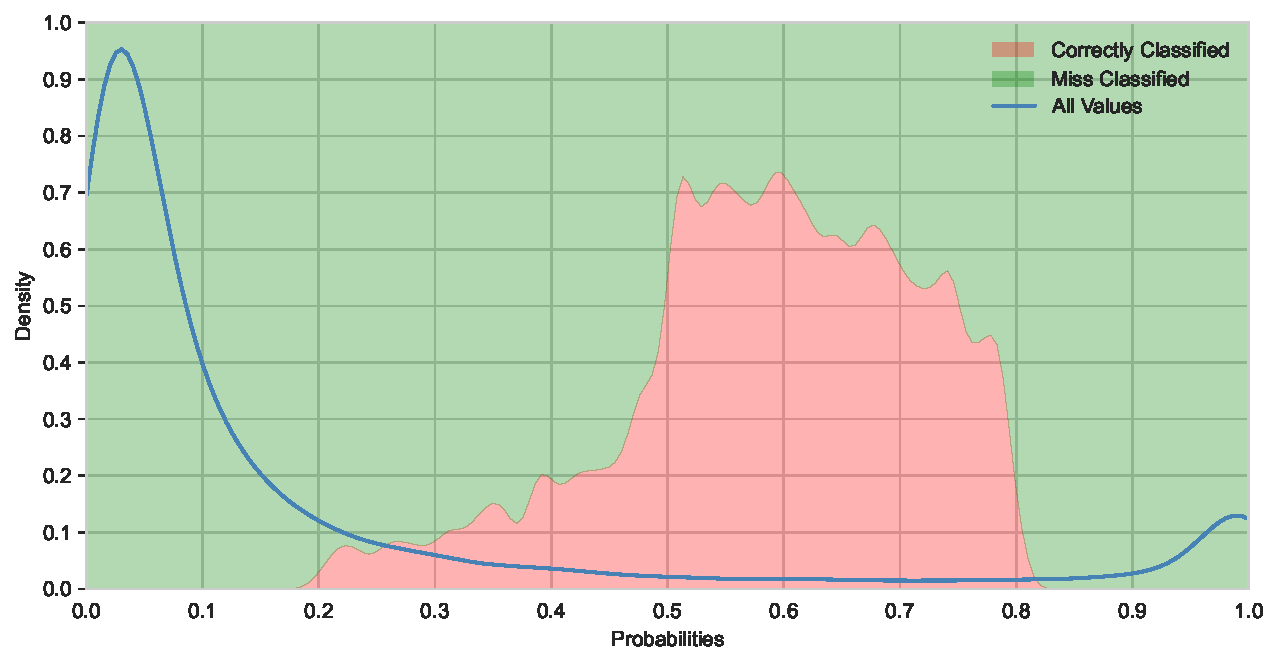
\includegraphics[width=\textwidth]{figures/predictionvalues_external.pdf}
 \caption[Prediction values of held-out datasets]{The distribution of the two held-out datasets and the kernel density estimations for the correct and incorrect values normalized between 0 and 1. Note that prediction values below 0.2 and above 0.8 are always treated as correct. Note that the kernel density line for all prediction values corresponds to the second y-axes that is not shown.}
 \label{fig:predictionvalues_external}
\end{figure}

\subsubsection{Dataset results}
%\textbf{URLs.}
We ran the web crawler for a little more than two weeks\footnote{We ran the crawler with a minimum of a thousand species each run, because of this we ran the crawler a little longer then two weeks, resulting in a large even number.}.
In these two weeks, we managed to query 20,000 different plant species.
Every species returned at least one URL.
For 20,000 species there are 519,197 unique URLs returned from 27,612 unique base URLs (URL homepage).
For 16,193 species, the URL returned text that could be classified.
3,807 species URLs did not return any useable text\footnote{The POWO website is excluded from the web crawler as this database is already available.}
In Figure \ref{fig:URL_distribution}, the distributions per species can be found.
Figure \ref{fig:URL_distribution_1} shows that around 17 to 33 unique URLs are found for most species.
Figure \ref{fig:URL_distribution_2} shows that multiple pages from the same base URL are retrieved for several species.
Finally, Figure \ref{fig:URL_distribution_3} shows that most URLs do not contain any description information for the species.
This happens when the headers of a certain page do not match anything from the species name, or the URL's text does not contain any description information according to the classifier. 

%\begin{figure}[htpb]
% \centering
% %\hspace{-0.5cm}
% 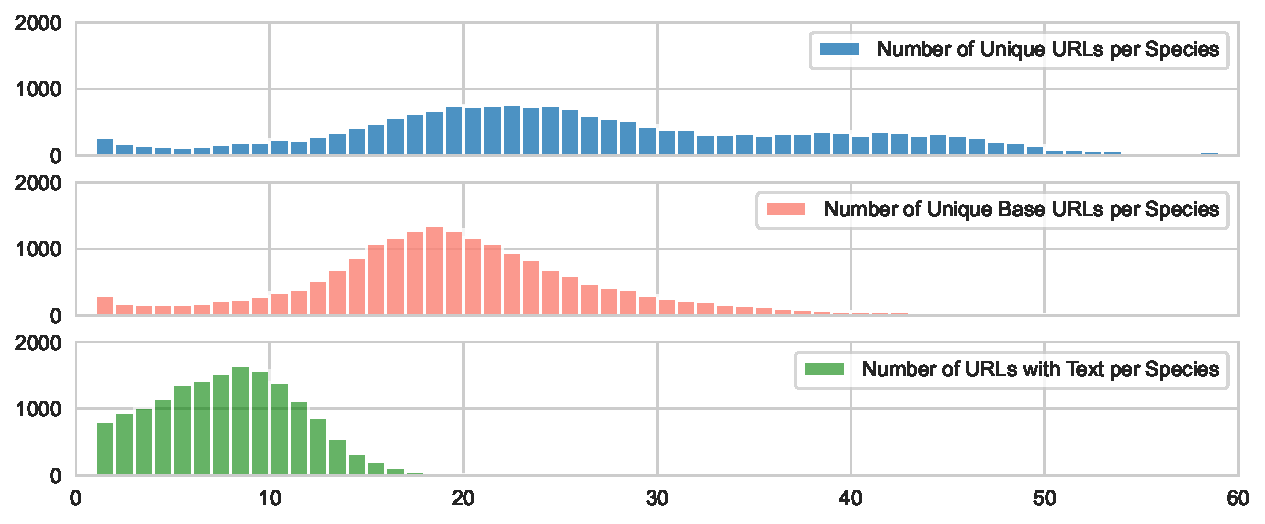
\includegraphics[width=\textwidth]{figures/URL_distribution.pdf}
% \caption[The URL, base URL and URLs with text per Species]{The distribution of the unique URLs per species, base URLs %per species and URLs with text per species.}
% \label{fig:URL_distribution}
%\end{figure}

\begin{figure} [htpb]
     \centering
     \begin{subfigure}[b]{1\textwidth}
         \centering
         %\hspace{-0.5cm}
         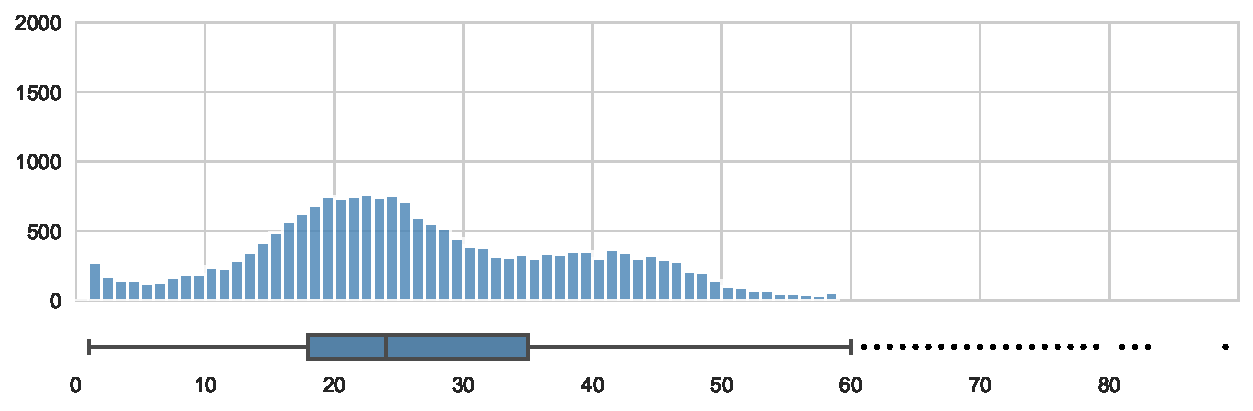
\includegraphics[width=\textwidth]{figures/URL_distribution_1.pdf}
         \caption{The number of unique URLs per species.}
         \label{fig:URL_distribution_1}
     \end{subfigure}
     \vfill
     \begin{subfigure}[b]{1\textwidth}
         \centering
         %\hspace{-0.5cm}
         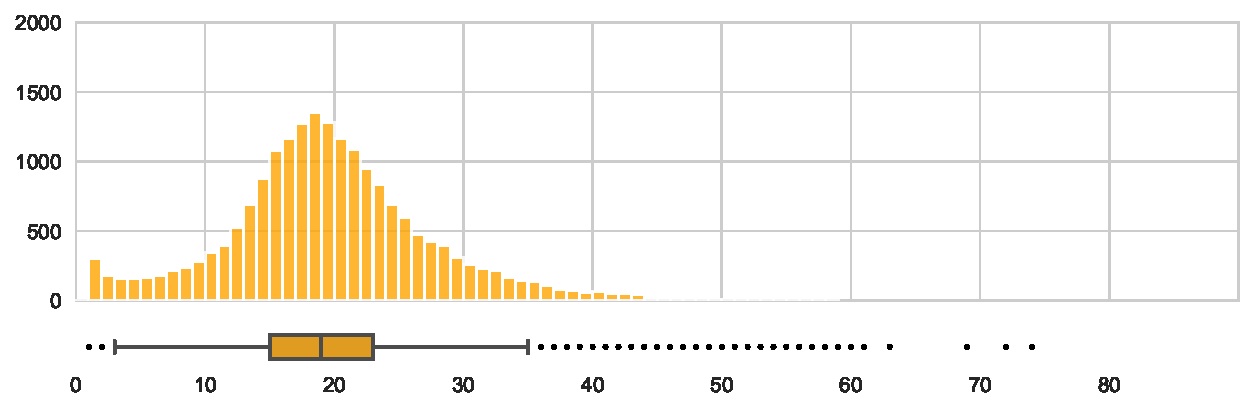
\includegraphics[width=\textwidth]{figures/URL_distribution_2.pdf}
         \caption{The number of unique base URLs per species.}
         \label{fig:URL_distribution_2}
     \end{subfigure}
     \vfill
     \begin{subfigure}[b]{1\textwidth}
         \centering
         %\hspace{-0.5cm}
         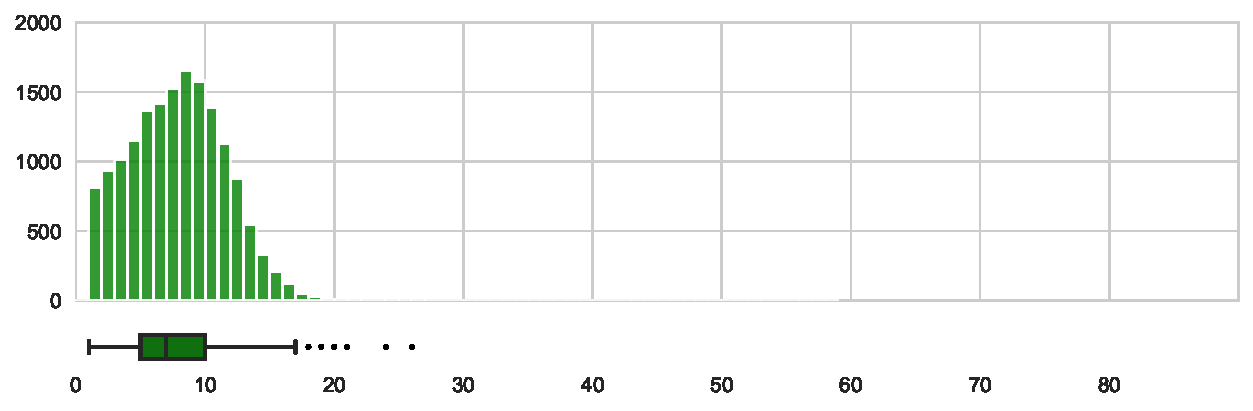
\includegraphics[width=\textwidth]{figures/URL_distribution_3.pdf}
         \caption{The number of URLs with text per species.}
         \label{fig:URL_distribution_3}
     \end{subfigure}
     \caption[The URL, base URL and URLs with text per Species]{The distribution of the unique URLs per species, base  URLs per species and URLs with text per species.}
     \label{fig:URL_distribution}
\end{figure}

In Figure \ref{fig:URL_top20}, the most returned base URLs can be found.
Research.net is by far the most returned base URL when querying species, followed by Academia.edu and the international version of Wikipedia.com.
Academic sites seem to contain the most information about the queried species.
\begin{figure}[t]
 \centering
 %\vspace{-2cm}
 %\hspace{-0.5cm}
 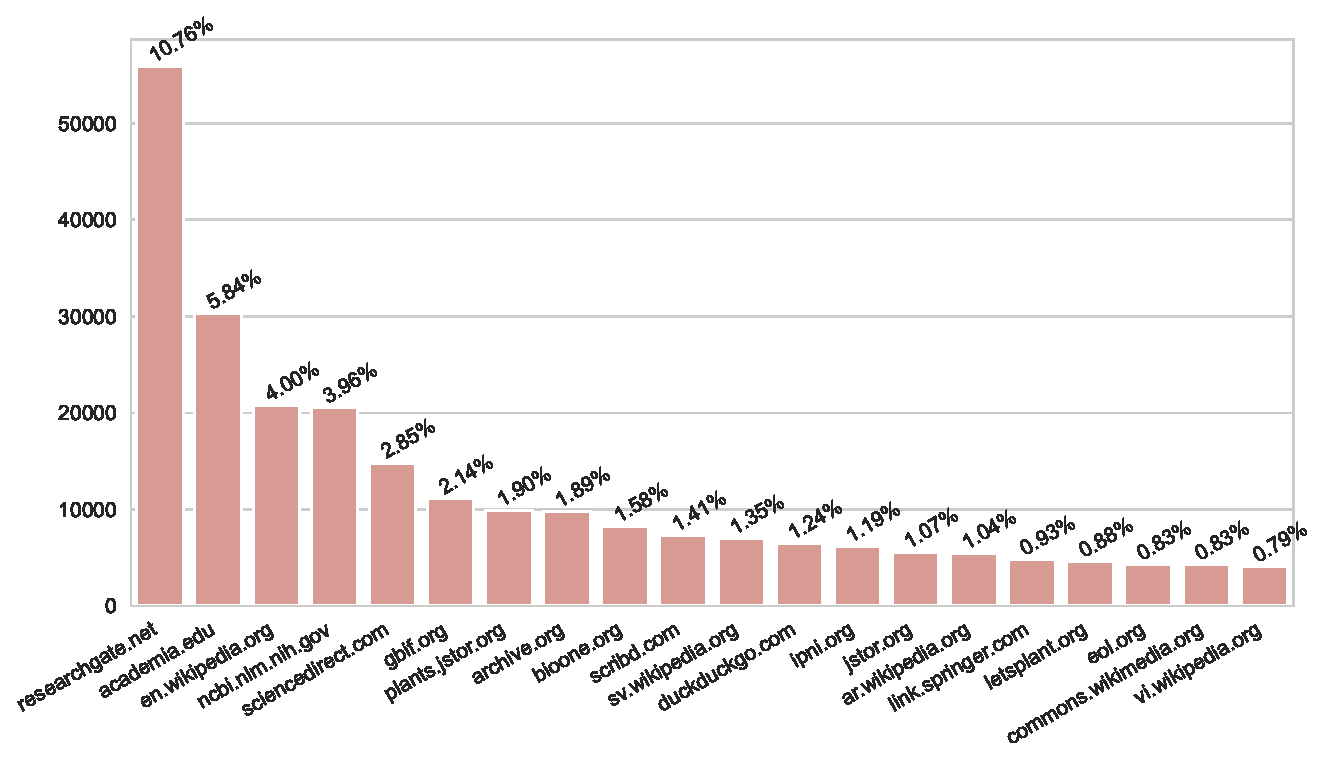
\includegraphics[width=\textwidth]{figures/URL_top20.pdf}
 \caption[The top 20 returned base URLs]{The top 20 base URLs that are returned the most. Above each bar the part of the overall total is plotted. This is the percentage compared to all unique base URLs. The top 20 unique base URLs make up 46.49\% of the total.}
 \label{fig:URL_top20}
\end{figure}

The URL titles are checked against the species name; if the species name exists within the title, the sentences are retrieved, resulting in 4,284,057 sentences.
We used the binary description classifier to classify these sentences, resulting in 218,106 sentences classified as a description.
We found description data for 14,557 different species.
We appended the data from the structured sources (PoWo, AgroForestry and Llifle) to these description sentences.
We dropped sentences that contained two words or less per sentence, resulting in 484,336 description sentences.

\begin{comment}

Figure \ref{fig:text_distribution} shows the distribution of sentences before and after classification.
In this figure the sentences are before classification without sentences from the structured datasets.
The description sentences contain all structured sources and the classified sentences from the web crawler.
\begin{figure} [htpb]
     \centering
     \begin{subfigure}[b]{1\textwidth}
         \centering
         %\hspace{-0.5cm}
         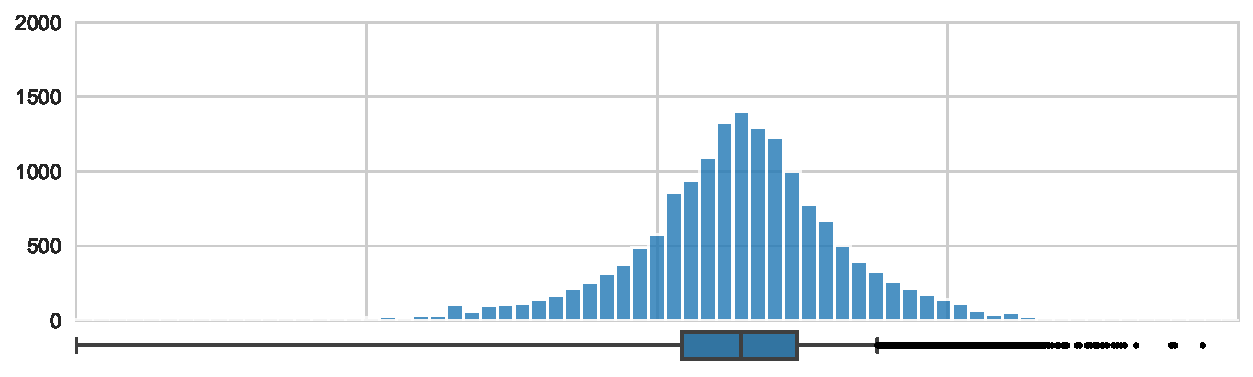
\includegraphics[width=\textwidth]{figures/text_distribution_1.pdf}
         \caption{The number of sentences per species.}
         \label{fig:text_distribution_1}
     \end{subfigure}
     \vfill
     \begin{subfigure}[b]{1\textwidth}
         \centering
         %\hspace{-0.5cm}
         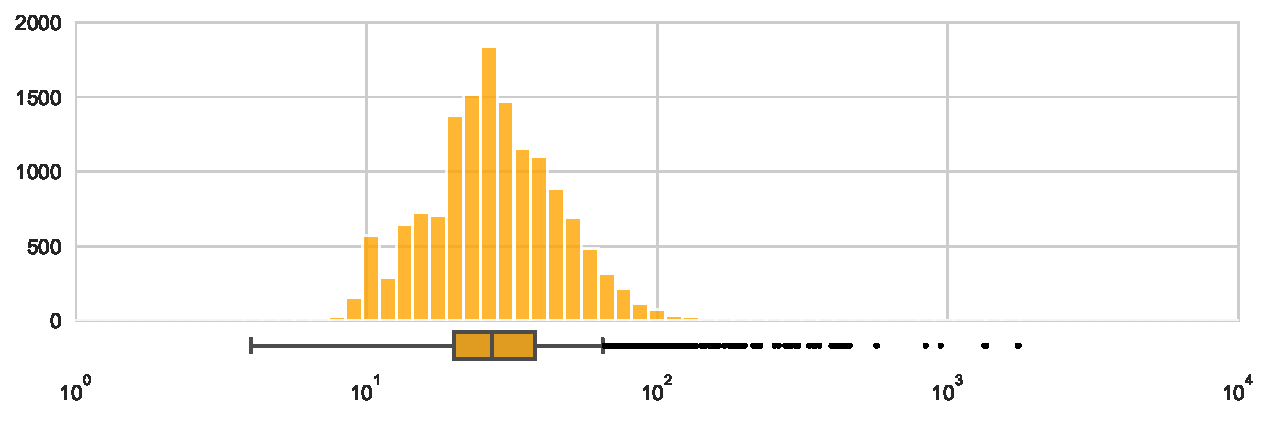
\includegraphics[width=\textwidth]{figures/text_distribution_2.pdf}
         \caption{The number of description sentences per species.}
         \label{fig:text_distribution_2}
     \end{subfigure}
     \caption[The sentences and descriptions sentences per species]{The sentences and descriptions sentences per species. The sentences per species are the sentences before classification. The description sentences are sentences that exceeded the threshold of .5 in the binary descriptions classifier. Note that the x-axis is a log-scaled axis and the boxplot is based on the normal values, hence the outliers on the right.}
     \label{fig:text_distribution}
\end{figure}
\end{comment}


\subsection{Key Word Extraction} \label{par:results_keywords}
In Figure \ref{fig:CUB_distribution}, the number of descriptions per bird for our created dataset and the CUB-200 dataset can be found.
For our dataset, we only display the 200 birds that exist within the CUB-200 dataset as these birds are used for further analysis.
The number of descriptions per bird is higher on average for the CUB data.
The CUB-200 dataset has a mean of 148.86 descriptions per bird, while our dataset had 119.21 descriptions per bird.
We did not find any descriptions for one Bird, the Cape Starling (Lamprotornis nitens).
\begin{figure} [htpb]
     \centering
     \begin{subfigure}[b]{1\textwidth}
         \centering
         %\hspace{-0.5cm}
         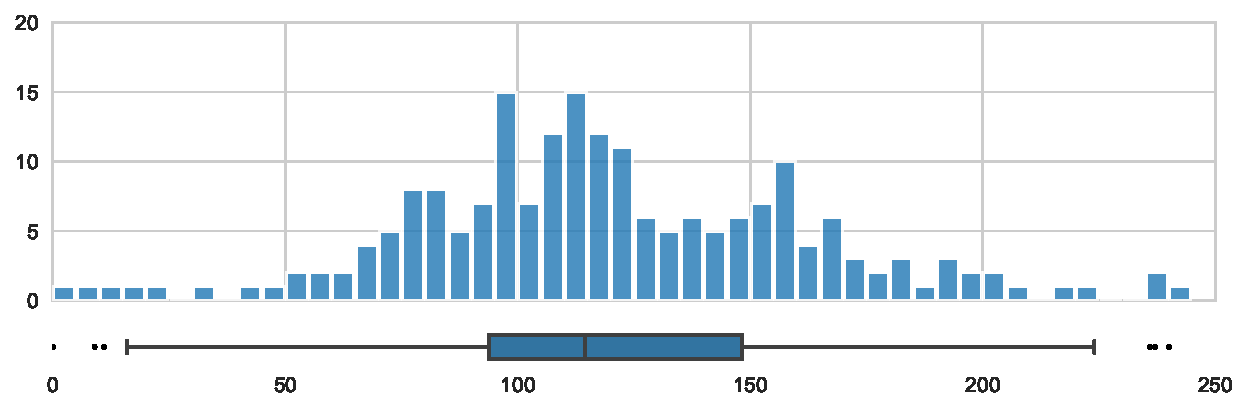
\includegraphics[width=\textwidth]{figures/CUB_distribution_BOW.pdf}
         \caption{The description distribution of the our dataset.}
         \label{fig:BOW_distribution}
     \end{subfigure}
     \vfill
     \begin{subfigure}[b]{1\textwidth}
         \centering
         %\hspace{-0.5cm}
         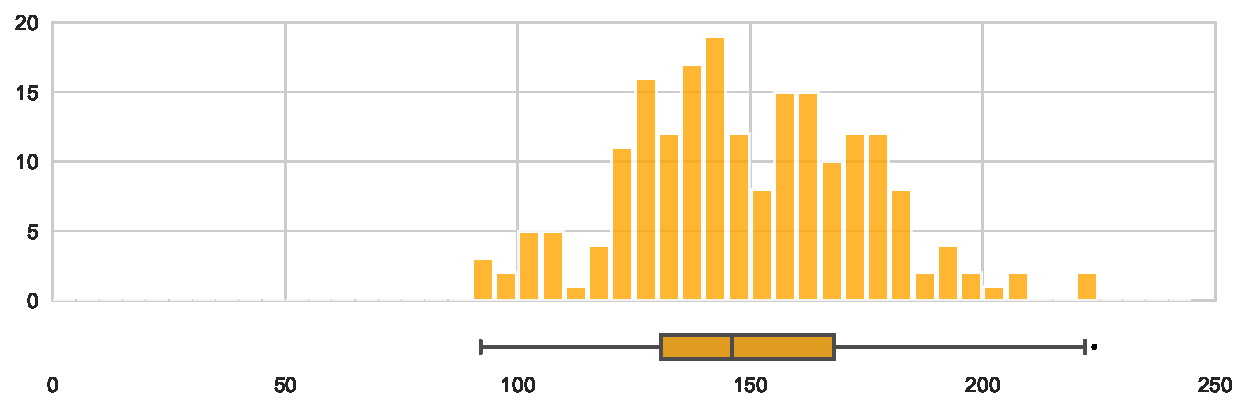
\includegraphics[width=\textwidth]{figures/CUB_distribution_CUB.pdf}
         \caption{The description distribution of the CUB dataset.}
         \label{fig:CUB_distribution}
     \end{subfigure}
     \caption[Bird description distribution]{The number of descriptions per bird for our data set that consists of random data and the Birds of the World dataset, and the CUB-200 dataset from the California Institute for Technology \autocite{welinder_caltech-ucsd_2010}. }
 \label{fig:CUBBOW_distribution}
\end{figure}


In Figure \ref{fig:hmean_violin} the results of computing the similarity of the attribution technique against the CUB-200 dataset can be found.
The values are sorted on the median values (lowest at the top, highest at the bottom).
All attribution technique distributions are scaled (the y-axis is removed for aesthetic reasons) and vary from 0.0 to 1.0.
PoS, in combination with dependency, has the highest harmonic mean, the highest normal mean and the highest median of all information extraction techniques.
\begin{figure}[htpb]
 \centering
 %\hspace{-0.5cm}
 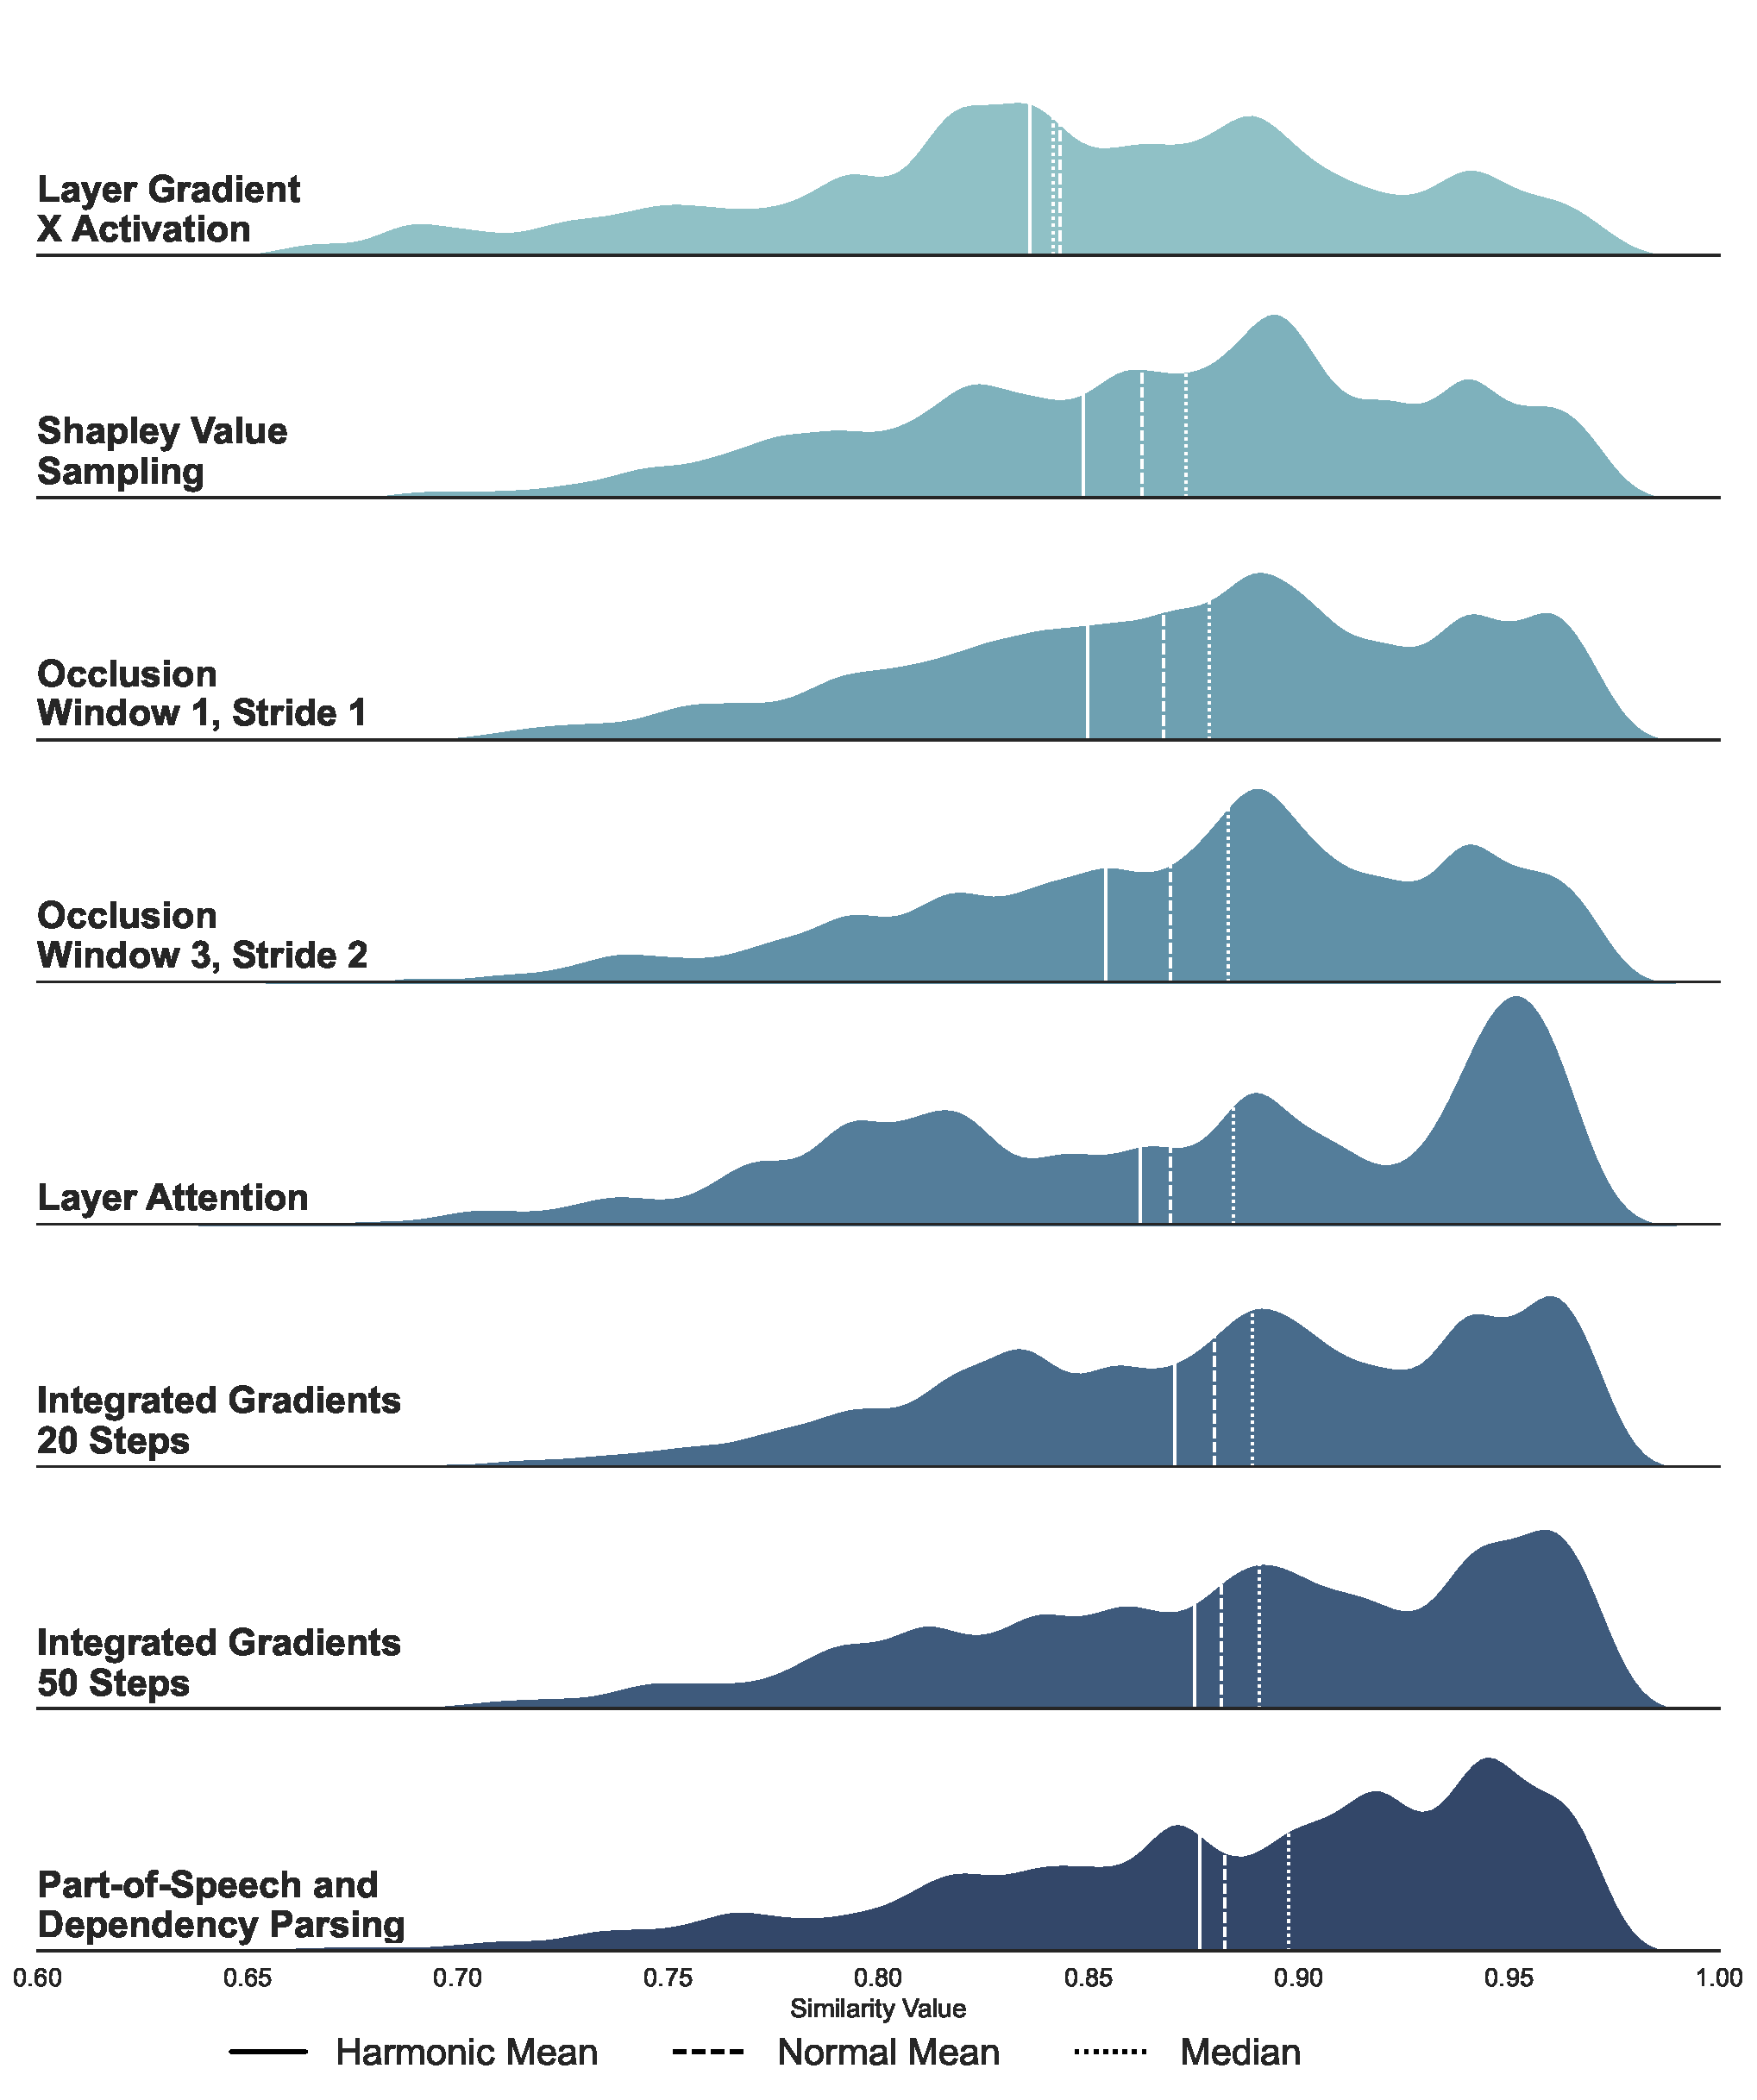
\includegraphics[width=\textwidth]{figures/densities.pdf}
 \caption[Similarity results]{The Results of computing the similarity of the different methods of our own dataset against the CUB-200 dataset. The distributions are coloured and sorted based on the harmonic mean.}
 \label{fig:hmean_violin}
\end{figure}


\subsection{Species Classification}
We found 547 common species between the PoWo dataset and the Llifle dataset.
219 species contain at least one description and are used to evaluate the dataset\footnote{There are a lot more overlapping species as we gathered around 30.000 species from the PoWo dataset and 20.000 from Llifle dataset, but these are common species that are described in both datasets.}.
The median of the correct group was -448, and the median of the incorrect group was -545.
The mean of the correct group was -921, and the mean of the incorrect group was -990.
The distributions in the two groups differed significantly (Wilcoxon Signed Rank = 15876422, n1 = 214, n2 = 214, P < 0.01, greater).
The negative log prediction values of the correct species are higher than that of the negative log values of the incorrect species. 
In Figure \ref{fig:Log_dist} the distributions and boxplots of the summed log values can be found.

\begin{figure}[htpb]
 \centering
 %\hspace{-0.5cm}
 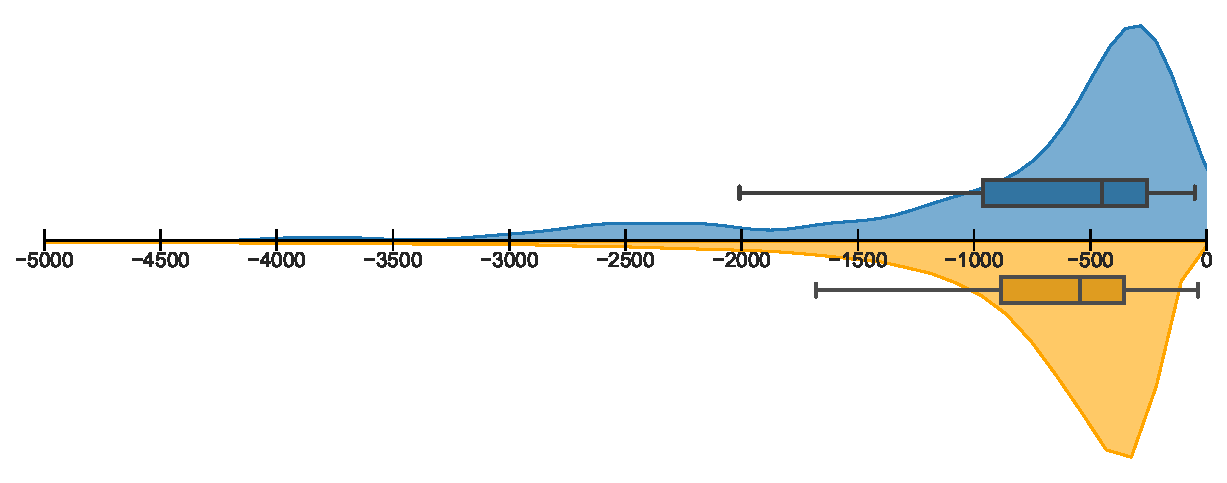
\includegraphics[width=\textwidth]{figures/log_plot.pdf}
 \caption[Log Distribution]{The summed log distribution of the species predictions. The blue values represent the correct species, and the orange values indicate the incorrect species. Note that outliers have not been plotted.}
 \label{fig:Log_dist}
\end{figure}


\subsection{Information Extraction}
We report the results of comparing our proposed workflow against the Palm Trait dataset and against the CUB dataset.
Second, we compare the manually created species identification matrices against our proposed workflow.

\subsubsection{Palm Trait Dataset}
In Table \ref{tab:palm_trait_binary} the metrics of the binary traits of the Palm Trait dataset can be found.
\begin{table}[htpb]
\centering
\caption[Palm Trait dataset Binary results comparison]{Palm Trait dataset Binary results comparison. Per binary trait we report Precision, Recall and F1 Score.}
\label{tab:palm_trait_binary}
\begin{tabular}{@{}lccc@{}}
\cmidrule(l){2-4}
             & \textbf{Precision} & \textbf{Recall} & \textbf{F1 Score} \\ \midrule
Climbing     & 0.952              & 0.976           & 0.964             \\ \midrule
Acaulescent  & 0.905              & 0.948           & 0.926             \\ \midrule
StemErect    & 0.924              & 0.452           & 0.560             \\ \midrule
StemSolitary & 0.833              & 0.681           & 0.714            \\ \midrule
StemArmed    & 0.838              & 0.911           & 0.873             \\ \bottomrule
\end{tabular}
\end{table}

In Figure \ref{fig:confusion_matrix_shapes} the confusion matrix for the shapes and in Figure \ref{fig:confusion_matrix_colours} the confusion matrix for the colours can be found.
Table \ref{tab:confusion_matrix_metric_table} contains the accompanying metrics for the figures and the missing values.

\begin{figure}[htpb]
    \centering
    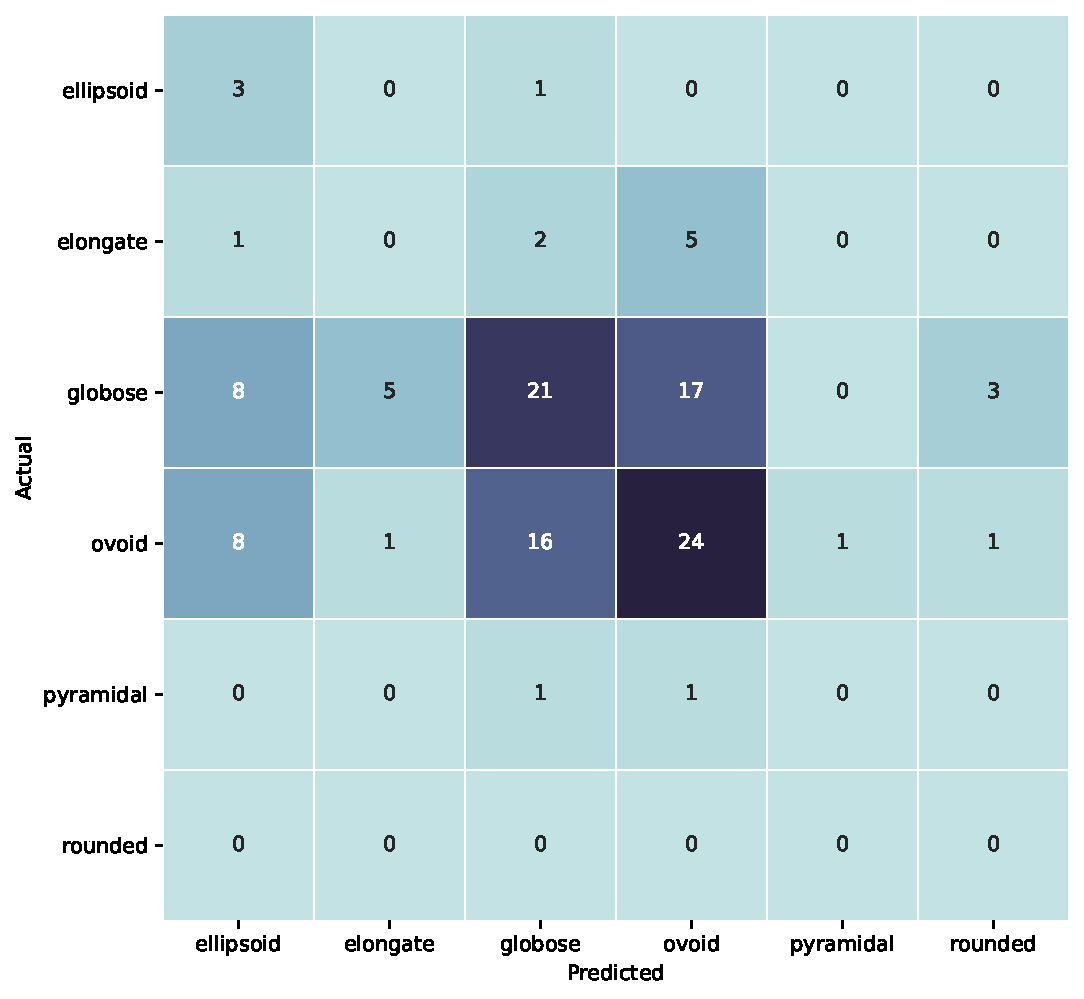
\includegraphics[width=0.85\textwidth]{figures/confusion_matrix_shapes.pdf}
    \caption[Confusion matrix shapes]{The confusion matrix for the shapes. On the Y-axis the values of Palm Trait dataset can be found. On the X-axis our values can be found. The accompanying metrics and the missing values can be found in Table \ref{tab:confusion_matrix_metric_table}.}
    \label{fig:confusion_matrix_shapes}
\end{figure}

\begin{figure}[htpb]
    \centering
    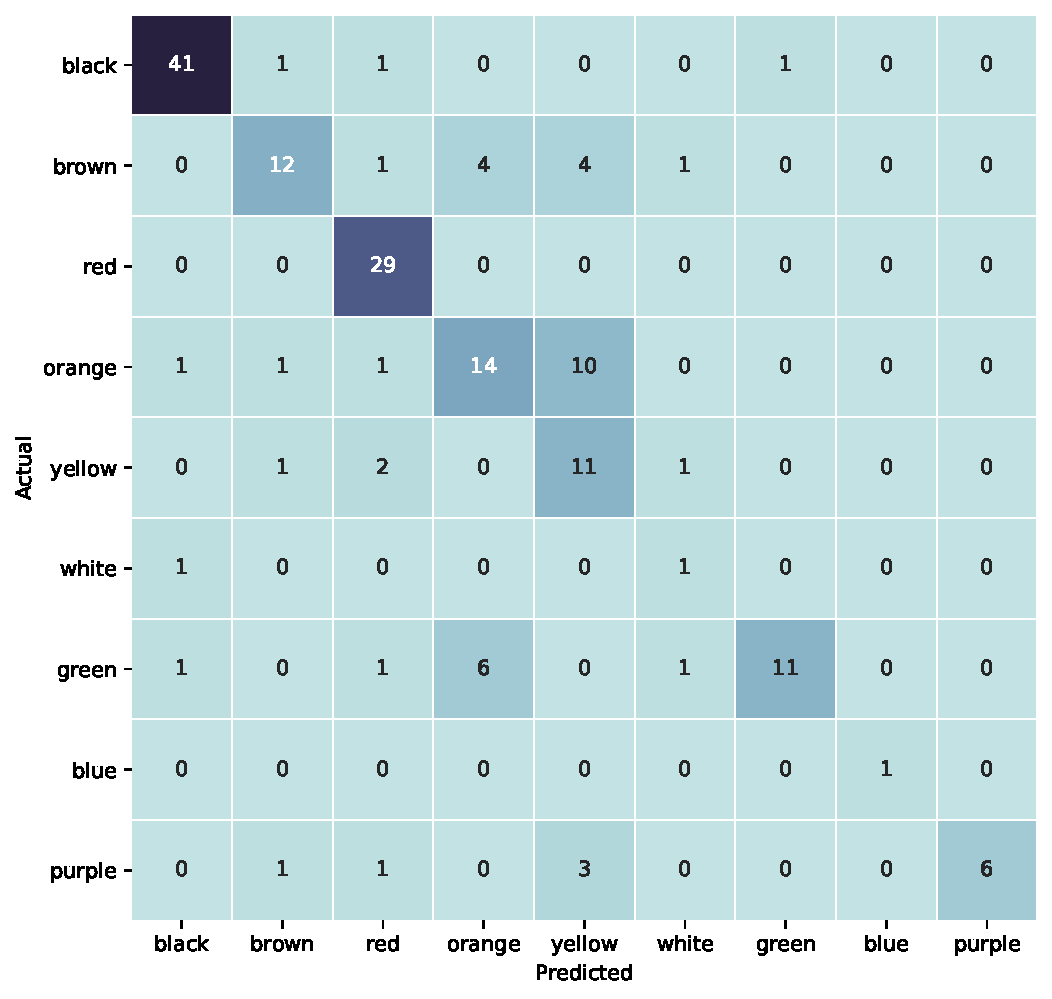
\includegraphics[width=0.99\textwidth]{figures/confusion_matrix_colours.pdf}
    \caption[Confusion matrix colours]{The confusion matrix for the colours. On the Y-axis the values of Palm Trait dataset can be found. On the X-axis our values can be found. The accompanying metrics and the missing values can be found in Table \ref{tab:confusion_matrix_metric_table}. Note that order of the values is roughly the same as that of the radiometric spectrum; similar colours are closer together in this confusion matrix.}
    \label{fig:confusion_matrix_colours}
\end{figure}

\begin{table}[htpb]
    \centering
    \caption[Accompanying metric for confusion matrices]{The accompanying metrics for the confusion matrix for the shapes (Figure \ref{fig:confusion_matrix_shapes}) and the confusion matrix (Figure \ref{fig:confusion_matrix_colours}) for the colours. Note that the Precision, Recall and F1 Score are bases on the confusion matrix without missing values.}
    \label{tab:confusion_matrix_metric_table}
    \begin{tabular}{@{}lcccc@{}}
    \cmidrule(l){2-5}
            & \multicolumn{1}{l}{\textbf{Missing}} & \multicolumn{1}{l}{\textbf{Precision}} & \multicolumn{1}{l}{\textbf{Recall}} & \multicolumn{1}{l}{\textbf{F1 Score}} \\ \midrule
    Shapes  & 129                                  & 0.450                                  & 0.193                              & 0.267                                 \\ \midrule
    Colours & 77                                   & 0.770                                  & 0.508                               & 0.595                                 \\ \bottomrule
    \end{tabular}
\end{table}


In Figures \ref{fig:stem_values}, \ref{fig:leaf_values}, \ref{fig:fruitlength_values}, \ref{fig:fruitwidth_values} and \ref{fig:petioleANDrachis_values} our found values versus the ground truth values of the Palm Trait dataset can be found.
The figures contain the difference of our value expressed as a percentage of the ground truth value.
Missing values are shown in the Figures as a dashed red line and extreme values (a difference greater than 25\% is shown with a red triangle).
A ground truth is available for every predicted value.
In a few ground truth cases contain a zero, when our model predicts a different value it will resulted in an infinitely large error percentage.

\begin{figure}[htpb]
    \centering
    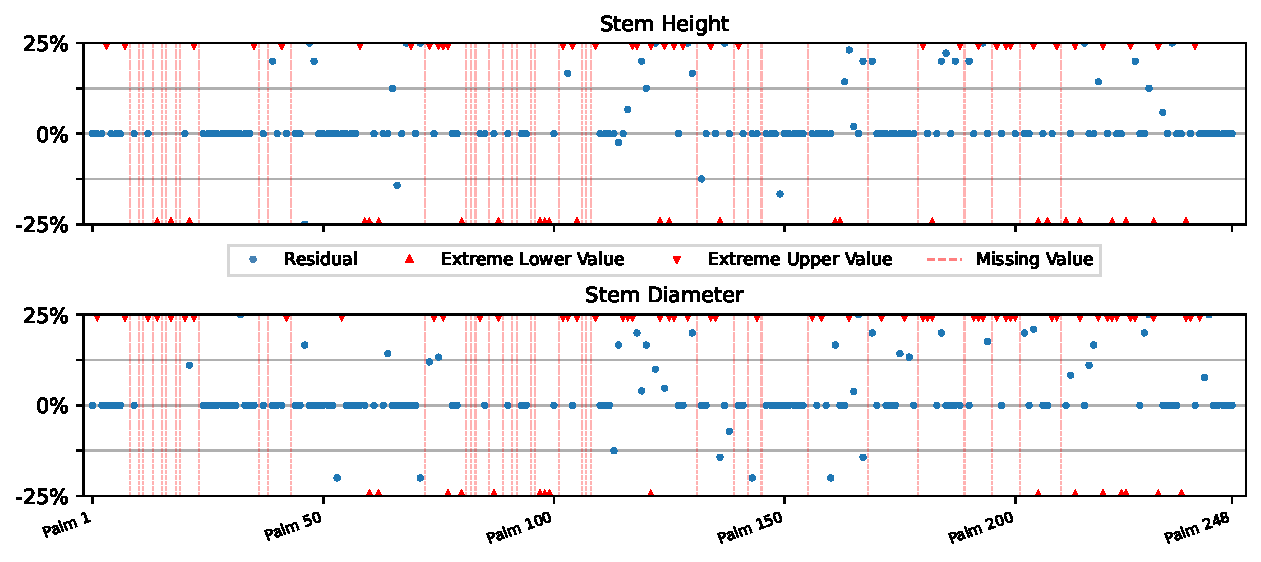
\includegraphics[width=1\textwidth]{figures/stem_values.pdf}
    \caption[Stem values ground truth vs predicted]{The the predicted stem values expressed as a percentage of the ground truth values. Extreme values (below or above 25\%) are not plotted and are indicated with a little triangle. A dashed vertical line indicates a missing value; the web crawler did not found any stem values for this palm species. Our approach resulted in 115 correct, 35 within 25\% 61 outside 25\% and 37 missing values.}
    \label{fig:stem_values}
\end{figure}

\begin{figure}[htpb]
    \centering
    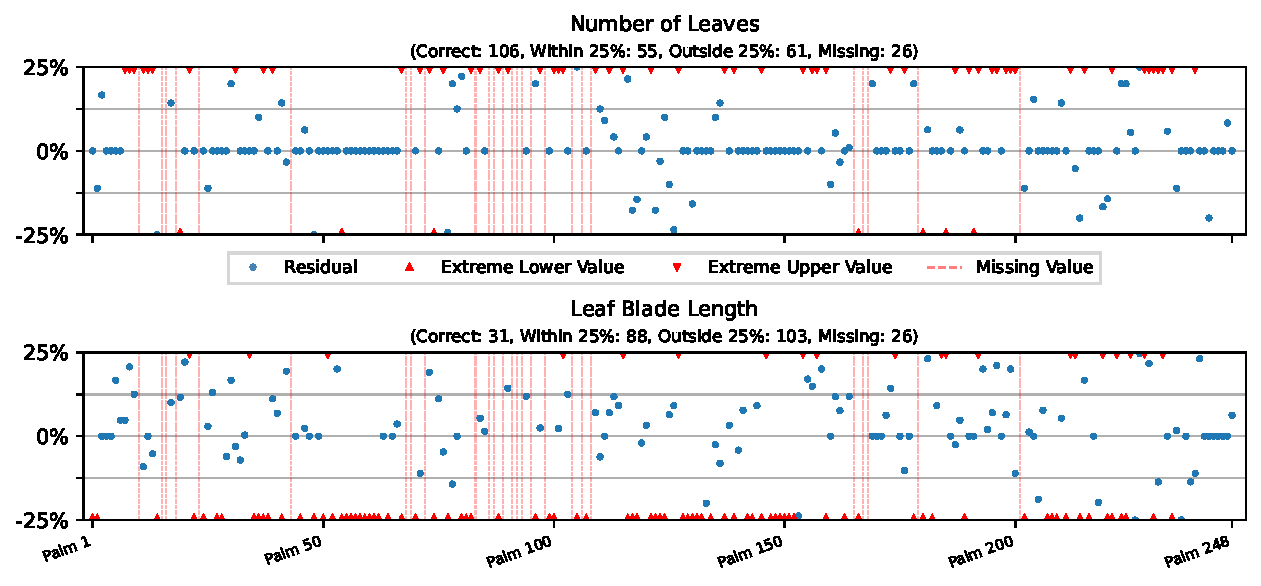
\includegraphics[width=1\textwidth]{figures/leaf_values.pdf}
    \caption[Leaf values ground truth vs predicted]{The the predicted leaf values expressed as a percentage of the ground truth values. Extreme values (below or above 25\%) are not plotted and are indicated with a little triangle. A dashed vertical line indicates a missing value; the web crawler did not found any leaf values for this palm species.}
    \label{fig:leaf_values}
\end{figure}

\begin{figure}[htpb]
    \centering
    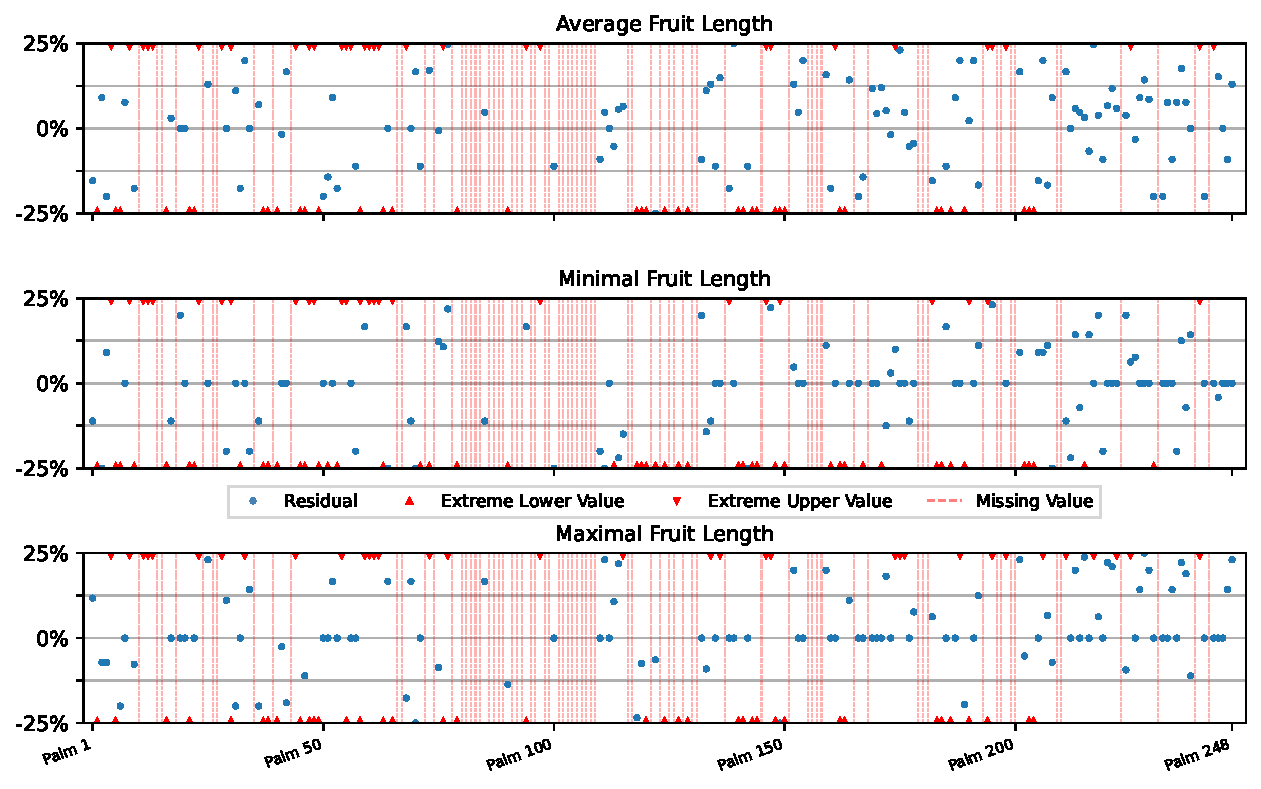
\includegraphics[width=1\textwidth]{figures/fruitlength_values.pdf}
    \caption[Fruit length values ground truth vs predicted]{The the predicted fruit length values expressed as a percentage of the ground truth values. Extreme values (below or above 25\%) are not plotted and are indicated with a little triangle. A dashed vertical line indicates a missing value; the web crawler did not found any fruit length values for this palm species.}
    \label{fig:fruitlength_values}
\end{figure}

\begin{figure}[htpb]
    \centering
    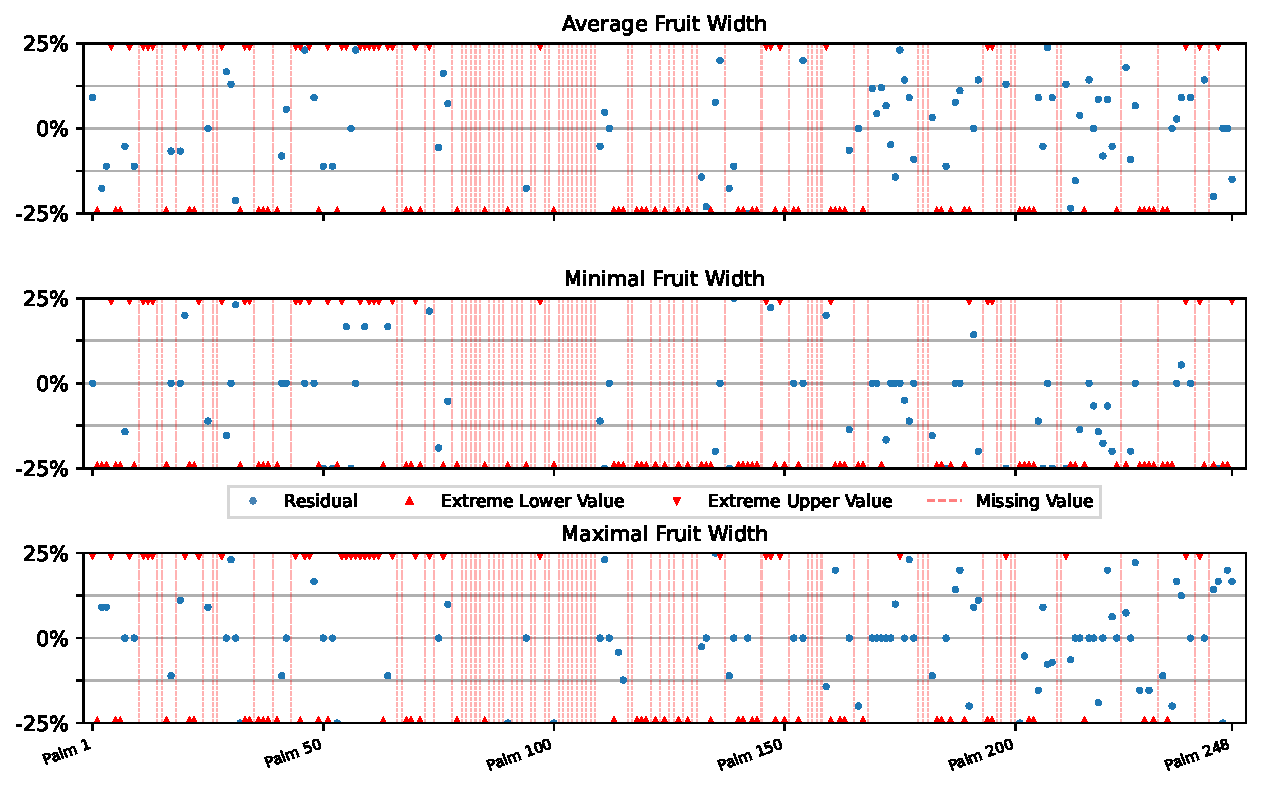
\includegraphics[width=1\textwidth]{figures/fruitwidth_values.pdf}
    \caption[Fruit width values ground truth vs predicted]{The the predicted fruit width values expressed as a percentage of the ground truth values. Extreme values (below or above 25\%) are not plotted and are indicated with a little triangle. A dashed vertical line indicates a missing value; the web crawler did not found any fruit length width for this palm species.}
    \label{fig:fruitwidth_values}
\end{figure}

\begin{figure}[htpb]
    \centering
    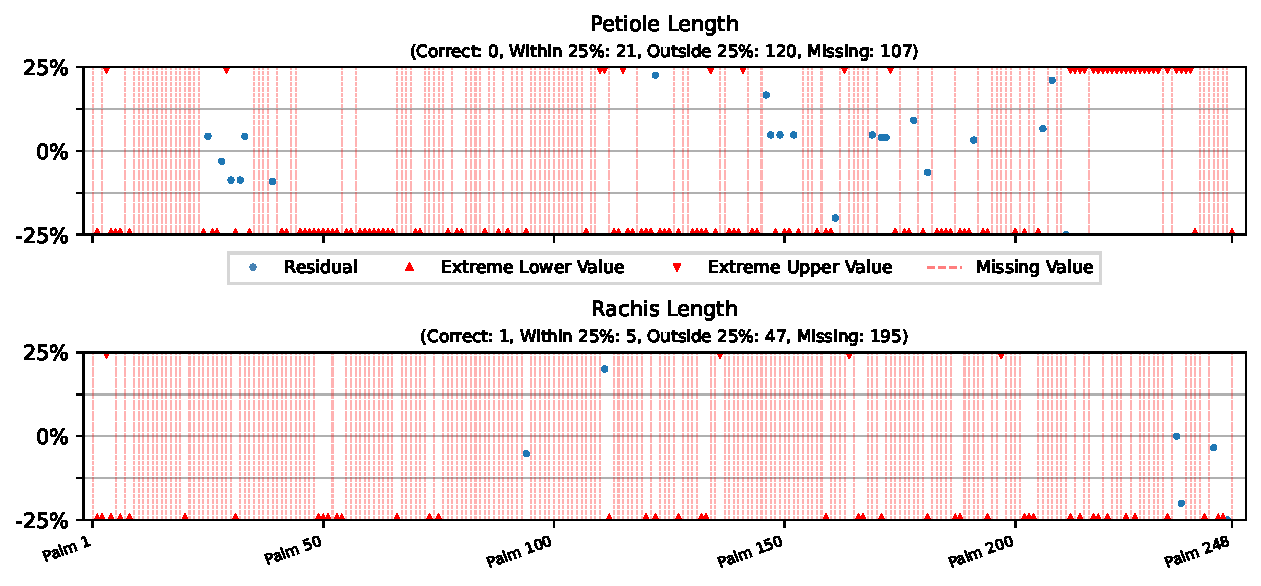
\includegraphics[width=1\textwidth]{figures/petioleANDrachis_values.pdf}
    \caption[Petiole and rachis values ground truth vs predicted]{The the predicted petiole and rachis values expressed as a percentage of the ground truth values. Extreme values (below or above 25\%) are not plotted and are indicated with a little triangle. A dashed vertical line indicates a missing value; the web crawler did not found any petiole length and rachis length for this palm species.}
    \label{fig:petioleANDrachis_values}
\end{figure}

\subsubsection{CUB-200 Dataset}
Figure \ref{fig:bird_ranking} contains the ranking of descriptions of each bird against all other birds of the CUB-200 dataset. 
The average ranking of our birds is 40.15.
There is a faint visible diagonal pattern visible, meaning that our data gathering approach does result in useful data. Ideally, every value in the diagonal line would equal one. In our case the average ranking value is 40.15, which would be better than random sampling from a distribution between 1 and 201.

\begin{figure}[htpb]
    \centering
    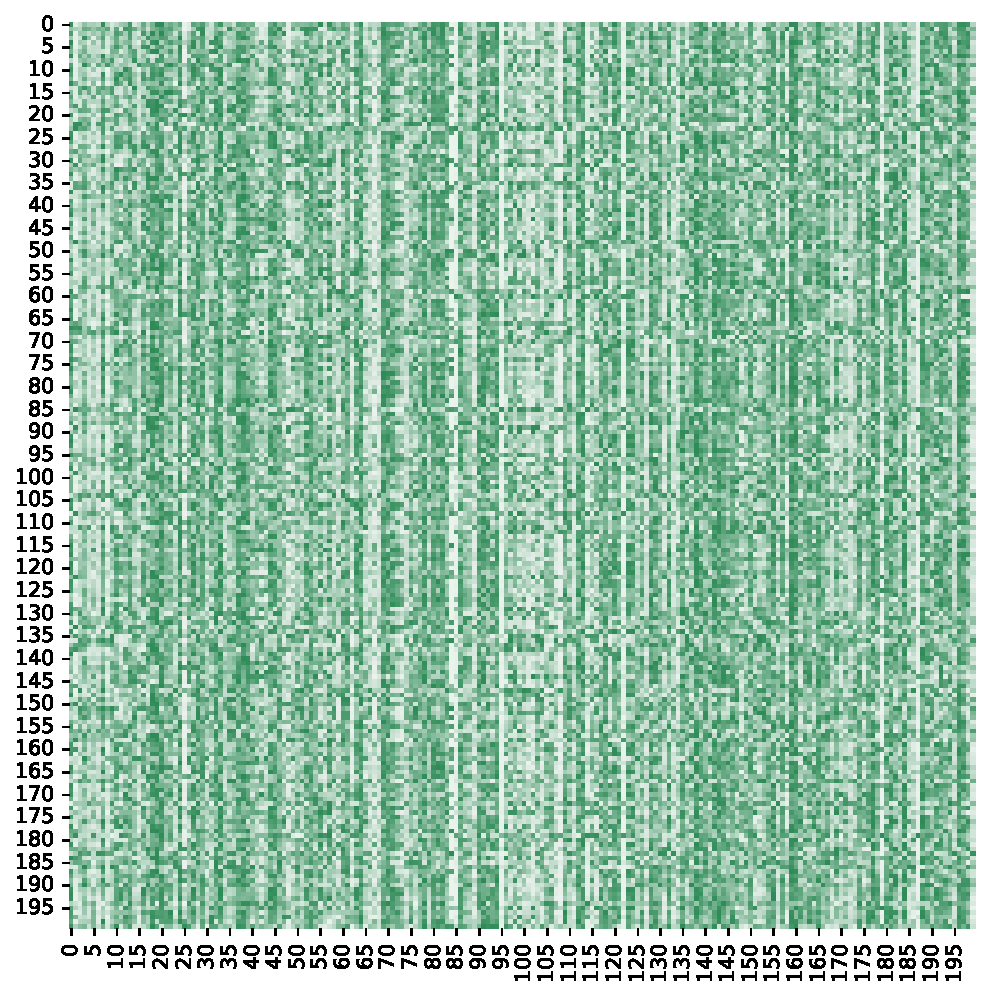
\includegraphics[width=1\textwidth]{figures/bird_ranking_v4.pdf}
    \caption[Ranking of our birds against CUB birds]{Ranking of the birds of our datasets against the birds of the CUB dataset. On the y-axis our birds can be found. Each bird is ranked against all other 200 birds of the CUB dataset. }
    \label{fig:bird_ranking}
\end{figure}


\newpage
\section{Discussion} \label{par:discussion}
\markboth{Discussion}{Discussion}

\subsection{Binary Classifier}
We gathered enough samples (See Figure \ref{fig:text_length_distribution}) to properly train a binary classifier.
Figures \ref{fig:text_length_1} and \ref{fig:text_length_2} show that the number of samples for the negative class is much higher than the positive class. 
After splitting the features into chunks of a random length between 10 and the text length, the data is still skewed; the non-description class is over represented in the data (see Figures \ref{fig:text_length_3} and \ref{fig:text_length_4}). 
This skewed data set could lead to problems as the classifier will not see enough underrepresented class samples.
The classifier will only update the parameters for the non-description class and still reach a good result on the test data.
Because of this skewness, we evaluated the dataset with a precision-recall plot (Figures \ref{fig:precision_recall_curve_test} and \ref{fig:precision_recall_curve_test_external}).
The binary description classifier performs excellently on the test dataset. 
The loss function of \textcite{reed_training_2015} (Equation \ref{eq:softloss}) seems to do an excellent job.
As shown from Table \ref{tab:precision_recall_metrics} and Figure \ref{fig:precision_recall_curve_test}, the classifier reaches an excellent AP and F-1 score on the left out-test set.
The classifier identifies almost all description text chunks from the data (recall).
The text chunks qualified as descriptions are almost all correctly classified (precision).

The classifier performs worse on the two held-out datasets. 
The returned results are still relatively high with a recall of 0.90; however, the precision is lower with 0.83; the returned labels are incorrect for 17\% of the time.
However, as both F-1 values exceeded the threshold value set at the beginning of this thesis, the model was deemed sufficient and deployed in the web crawler. 
%However, we have some suggestions to improve the binary classifier in future work.
%Unfortunately we due to lack of time we only implemented of \(\beta\) of 0.80. 
%By starting with a lower \(\beta\) and gradually increase \(\beta\) during the parameter optimisation %process, the model might optimise the parameters better as it gets penalised less hard.

\subsubsection{Description Classifier Accuracy}
With the two held-out datasets, we processed the text the same way as we would have when the text was processed by the web crawler. 
We clean the text and split the text into single sentences with the sentecizer of \textcite{honnibal_spacy_2020}.
As we do not have the ground truth labels of this dataset, we implemented Equation \ref{eq:softloss_ifthen}.
This equation will treat prediction values with a 0.8 or higher as correct\footnote{It actually changes the label of the sample.}.
The classifier still performs very reasonably on the two left out datasets.
However, with an F1-score of 0.86, the classifier performs worse than the test dataset.
This performance issue is likely to occur due to the following reasons:

First, this could be a classic example where a model learns to predict over-represented class in the dataset.
%The model has seen more sample of non-description data than is has seen description data.
During the training process, the model has seen more samples of the negative class.
The model updates the parameters based on the loss function and does so equally for both classes.
As the model has seen more samples of the negative class, it better learns to predict the negative class.
In our case, the negative class is also over represented in the dataset during training (See Section \ref{par:results_binary_classifier}).
The parameters are better optimised for the over represented class, i.e. the negative class.
Figure \ref{fig:predictionvalues_external} clearly shows that the misclassified samples are much higher for the positive samples (description values) than for the negative samples. 
The data distribution for the two-left out test sets is also skewed, as can be seen from Table \ref{tab:precision_recall_metrics}.
Figure \ref{fig:predictionvalues_external} show that the output probabilities for the two held-out datasets also follow this skewness; far more prediction values are pushed towards zero than towards one.
The model learned to predict the negatives better than the positive values.

Second, the data preparation could cause performance issues.
During the training of the binary classifier, the text is randomly split into chunks. 
In some cases, this will result in text chunks that will contain part of a description and something else.
The text data is not all in the correct place of a paragraph, e.g. descriptive data about species can also occur in the introduction (also see Section \ref{par:reedloss}).
Even with an appropriate \(\beta\), the model cannot optimise the parameters correctly as a single feature contains information from both labels.
This will result in a model that cannot optimally utilise the loss function from \textcite{reed_training_2015}, as high prediction values will be less likely to be reached.
Thus the loss function is not used to its full extend.
%The model will perform well on correctly labelled sentences, but its prediction values will be less certain.
This might explain the lower F-1 score of the classifier on the two held-out datasets.
Like with the training data, the held-out datasets will contain mislabelled sentences as the text is messy (again, see Section \ref{par:reedloss}).
The parameters are not fully optimised, and thus the model will not reach the \(\beta\) threshold of 0.8, resulting in an incorrect prediction, even when the sentence is a description.
%This will result in mislabelled sentences, where the model cannot use the high prediction value in case it is certain about a prediction, because the parameters are not fully optimised.
It would make sense to split the text into smaller chunks or even single sentences during the training of the classifier in future research.
This would make sure a feature is more likely to contain just a single label and features do not contain multiple pieces of information.
During the training process of the model, the parameters are better optimised, resulting in higher prediction values.
During testing, the binary classifier can now utilise these higher prediction values.
mislabelled sentences of external test sets are now sooner labelled correctly.
During testing, one could also use a lower \(\beta\) or use the hard loss equation of \textcite{reed_training_2015}.
We used the same \(\beta\) during training and testing.
However, during the training, we used the soft loss of \textcite{reed_training_2015}, whereas, during testing, we used a modified version of their hard loss.
The soft loss equation directly calculates regression targets for each batch, where the hard loss version is allowed to change the label if the set threshold is reached.

Third, the lower F1-value could be specifically related to the two held-out datasets from Llifle and Agroforestry.
Overall the classifier performed well; Figure \ref{fig:predictionvalues_external} show that most prediction values are pushed towards either zero or one.
However, Figure \ref{fig:predictionvalues_external} also shows that more samples are mislabelled between the threshold value of 0.5 towards 0.8 than below 0.5 and above 0.2.
Testing the misclassified values below 0.5 and above 0.5 against each other does confirm that misclassified values above 0.5 are significantly higher than below 0.5.
A possible explanation is that paragraphs that are labelled as descriptions (because of their header) have relatively more non-description sentences than non-description paragraphs that have description sentences.
In this case, the classifier performs worse because of incorrect labels.
When the prediction values of the classifier stay below the set \(\beta\), the sentences will be mislabelled as the model is not allowed to change the label.
To test this theory, one could test the classifier on addition datasets that are completely separated from the training process.
Most likely, it is a combination of the three aforementioned issues that cause the model performance to hamper slightly.


\subsubsection{Description Data Origins}
As can be seen from Figure \ref{fig:URL_distribution_1}, the web crawler did not find many URLs per species; according to the boxplot, most values lay between 17 and 33.
As far as we know, there is no literature available on the number of online available databases and websites that contain descriptions, but these numbers do not seem that high.
At time of writing, a bottleneck of our AI system is the web crawler.
We currently use Bing and DuckDuckGo to search the web for species descriptions.
However, as we do not have access to official API's we only use the results of the first pages, this severely limits the number of results.


The number of unique base URLs is even lower in Figure \ref{fig:URL_distribution_2}.
This means that the same base URL is returned multiple times for some species. 
Reasons for this could be that a web page creates a unique link for every paragraph, e.g.base link/species/intro and base link/species/habitat for a single species.
However, as this is not the scope of this thesis, we did not further investigate why the same base URL is returned multiple times for several species.

Another reason could be that some web pages are returned that do not correspond to the queried species and still manage to slip through.
We first split the species name and the header title and create an intersection between both.
In most cases, this will work correctly; however, this could sometimes lead to a failure, e.g., in the case of the queried species' Somateria spectabilis' and the returned title name' Somateria mollissima'.
In this case, the page will slip through because both names contain 'Somateria'
We do force the query with brackets to contain the full species name in the search, but this fails if another web page refers to the queried species.
In future research, it would be interesting to research how much correct content is returned when querying species and which search engines return the best result. 
Another option would be to store the extracted data under the species' title page and determine which species are the same. 

For most species, the number of useful URLs, i.e. at least one descriptive sentence is found, lies between 5 and 10, as shown in Figure \ref{fig:URL_distribution_3}.
About two-thirds of the URLs found do not contain any useful information for this thesis.
Not a single description is found on the web page in these cases.
This seems rather low.
We expected that most returned websites contain some descriptions with the constructed queries. 
These low values could be related to the search engines used in this thesis (DuckDuckGo and Bing).
It could also be related to the constructed queries.
During the crawling, we constructed several queries that are used to retrieve information from the search engines.
However, we did not investigate, which combination of 'species' + 'keyword' would result in the best informational retrieval.

More time should be devoted to building a better web crawler in future research. 
About two-thirds of all URLs retrieved does not contain any useful information.
A lot of information is also stored in PDF files and text files, which are not used in this thesis (See Section \ref{par:future} Recommendations \& Future Work).

\subsection{Information Extraction }
As can be seen from Figures \ref{fig:BOW_distribution} and \ref{fig:CUB_distribution}, the overall distribution is somewhat equal for both datasets.
The CUB dataset does seem to be more consistent in the data distribution.
The CUB dataset has a single outlier, whereas our dataset has multiple outliers, and has a lower $\sigma$ compared to $\mu$ then our dataset.
This does influence the comparison values, but does influence the conclusion.
We first match select a bird in both datasets, and after, this we match each part against each other.
If there is no (no part) data available in the BoW dataset, it will not match against the CUB-200 dataset, and no similarity value will be computed.

\subsubsection{Information Extraction Techniques}
Figure \ref{fig:hmean_violin} shows that PoS in combination with dependency parsing yields the highest similarity between the BoW dataset and the CUB-200 set.
The Integrated Gradients technique is a close second. 
According to \textcite{sundararajan_axiomatic_2017}, 20 to 300 steps are needed to best approximate the integral within 5\%.
Due to computational power limits, we only used 20 steps and 50 steps to approximate the integral.
As this was mainly to see which attribution techniques gave the best result, we did not further investigate if a higher number of steps would yield better results (although it is highly likely as the similarity values seem to shift when the number of steps increases, but the question is how much we already approximated the integral with 50 steps).
We did not test if the sum of the attribution is approximately equal to that of the difference between the input and baseline vector.

Layer Gradient X Activation, Shapely Value Sampling and the occlusion techniques with varying windows and strides did not yield good results. 
Their values are centered around 0.80, while the values of Part-of-Speech tagging and the integrated gradients techniques lay around 0.88.
These techniques are originally developed for images and not for text and may not capture the necessary features of the textual vector embeddings.

Part-of-Speech tagging in combination with dependency parsing yielded a slightly higher overall harmonic mean than the integrated gradients techniques.
This technique no longer uses information from the trained model, instead it uses another pretrained transformer based model to extract the necessary features of the text samples.
%We used a custom script based on the package of \textcite{honnibal_spacy_2020} to extract the necessary tags.

\subsubsection{Part-of-Speech Tagging \& Dependency Parsing}
%The PoS tagging is now based on the Python package of \textcite{honnibal_spacy_2020}.
%They used a transformer based approach to train the models \autocite{wolf_huggingfaces_2020, vaswani_attention_2017}.
%We used their interpretable output in combination with a rule-based system to extract to most important information about parts.
%However, as both distillBERT and their models are based on the transformer model of \textcite{vaswani_attention_2017}, the semantic output of their models might already be present in the vector representations of the sentences.
%In future work it might be possible to directly use a transformer based model to extract the necessary data from the sentence instead of building a rule-based system.
%The information might even be already present in the output vectors of a trained BERT model as the model of \textcite{wolf_huggingfaces_2020} is also based on BERT.
We used PoS to extract information from sentences as this gave the best results as can be seen in Figure \ref{fig:hmean_violin}.
By first matching nouns against an export glossary containing botanic terms, we were able to filter out misclassified sentences and extract information per part of each sentence.
We used this information to create a knowledge graph per species (see Figure \ref{fig:kngraph_unweighted} for an example of a single graph\footnote{For 500 Mediterranean tree species we have graphs available per part.}). 
These graphs are then again used to reconstruct sentences and predict a species (See Figure \ref{fig:probs_nonstacked} and Figure \ref{fig:probs_stacked}).
We release our code for the rule-based PoS tagging in combination with dependency parsing.

PoS tagging in combination with dependency parsing has proven to be exceptionally difficult.
Ideally one would extract nodes and relations that only contain a single word per node or relation\footnote{In the case of a compound it a node could contain more words, like the example of the "Brown bear".}.
This would allow for more sharing nodes between the species. 
In this thesis we did not process all the text into single words representing a node.
E.g. in the example of Figure \ref{fig:kngraph_unweighted} there is a triple containing "capsule", "has\_property"\footnote{This relation is not visible in Figure \ref{fig:kngraph_unweighted} due to aesthetic reasons.} and "beaked by persistent style".
This triple could be processed much further by combining the verb of the second node "beaked" and the agent "by" into the relation "beaked by".
The second node should by changed to "style".
Finally a new triple should be created: "style", "has\_modifier" and "persistent", resulting in Figure \ref{fig:kn_discussion}
\begin{figure}[htpb]
 \centering
 %\hspace{-0.5cm}
 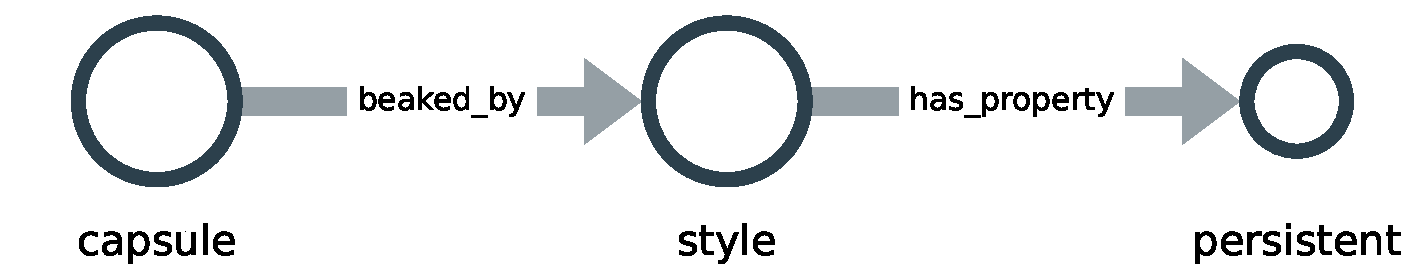
\includegraphics[width=0.6\textwidth]{figures/kn_discussion_example.pdf}
 \caption[Processing triples into singular words]{By further processing triples, every node and relation would exist out of one word allowing for more common traits across species.}
 \label{fig:kn_discussion}
\end{figure}

In future work, a trade off between needs to be made in the number of nodes and relations.
Limiting the the number of nodes and relations would result in more overlap between species; species can share more common traits.
In the case of 'up to 5 cm long', and 'to 5 cm long', the nodes should be joined into a single node to enhance species prediction (also see the next section about Species Predictions).

In the case of relations between the nodes choices have to be made. 
By allowing complex relations, like the relation "beaked by" in Figure \ref{fig:kn_discussion} a rigorous ontology will be created.
This ontology can contain complex information about species, but will again result in less shared traits as the information can still be quite complex and unique.
"Beaked by" is a valid and informational relation, but it will depend strongly on the descriptive text if such a relation will be found.
By creating simpler ontology, that only contains properties, more traits can be shared across species. 
The benefits of such a simpler property graph is also that is easier to maintain as most relation are the same (e.g. "has part", "has property").
In his case, the relation "Beaked by" will be changed into "Has part" (or something similar).



%The model seems to learn to predict a species based on two different datasets better than a random guess.
%We only assessed if the prediction values of the model were better than a random classifier, as this would be impossible.
% More explaining


% Something about the similarity?


%Since the PoS information extracting has proven to give decent results, duplicate information becomes less important as parts and traits can be shared across different species.

\subsubsection{Palm Trait Dataset Comparison}
We used several techniques to compare the Palm Trait dataset of \textcite{kissling_palmtraits_2019} to our data retrieved and constructed by our AI system.
The Palm dataset consists of multiple different variables as we described in Section \ref{par:palmtrait_methods}.


\noindent
\newline
\textbf{Numeric variables.}
In the Palm Trait dataset, we searched for the closest value in case of numeric values.
This works fairly well in the case of traits like the 'Stem Height', 'Stem Diameter' and 'Number of Leaves' as can be seen in Figures \ref{fig:stem_values} and \ref{fig:leaf_values}.
For most palm species a value is found, and our approach even yields the exact same value as the value described in the Palm Trait dataset several times. 
These traits are relatively simple\footnote{'Simple' as in everybody know what is meant, when this trait is presented.}.
It is relatively easy to obtain information about these traits.
When a web page contains any information about a palm trait, most of the times the simple traits are described.
This makes it easy for our approach to find the correct, or a close value for the species.

Plant traits, like 'Leaf Blade Length', 'Fruit Length and 'Fruit Width', seem to be more difficult to obtain. 
Compared to the simpler traits, there are a lot more missing values.
'Stem Height' and 'Stem Diameter' both have 37 missing values, 'Number of Leaves' only has 26 missing values, while 'Fruit Length' and 'Fruit Width' both have 72 missing values.
In these cases it is likely that these traits are less described by the web pages that we queried.

The Palm Trait dataset has three different ways to describe length and width: minimal, average and maximal length and width.
We did not check if there are multiple values available for each part for each species.
When comparing our data, it is possible that e.g. we found a fruit length value of '25 cm' and this is matched against the minimal, average and maximal fruit length values, as it is the closest value for all of them.
It is even possible (and highly likely) that the fruit length value is used to match against one or several fruit width values and vice versa.

When our approach returns a value, we (at this moment) do not know anything about the unit of this value, this applies to all numeric values from the Palm trait dataset.
The returned value for, e.g. the fruit width, could be 25 cm, 0.25 m, or it could even be expressed in millimeters. 
This could account for several larger outliers in Figures \ref{fig:stem_values}, \ref{fig:fruitlength_values}, \ref{fig:fruitwidth_values} and \ref{fig:petioleANDrachis_values}.
The same applies for imperial units (e.g. feet, inches).
The Palm trait dataset uses the metric system, so we need to convert them to metric values.
As long as the unit of measurements is provided in the descriptions (feet, meters), we can convert them to a common unit.
The unit is an 'appositional modifier' of a noun, or an 'adjectival complement' of a verb that describes a noun ('normal subject').
If the the unit contains any values, they are always joined by as an 'numeric modifier', allowing us in future work to correct these values.
%For specific traits like 'Rachis length' even fewer values are returned.

\noindent
\newline
\textbf{Multi Class Variables.}
Figure \ref{fig:confusion_matrix_shapes} contains the confusion matrix for the shapes of the fruit and Figure \ref{fig:confusion_matrix_colours} contains the confusion matrix for the colours of the fruit.
In Table \ref{tab:confusion_matrix_metric_table} the accompanying metrics for both Figures can be found. 

I case of the fruit shape, our AI system misses quite a few values. 
With 129 missing values, a little over 50\% are missed for the selected palm trees.
Our approach does seem to pick up a signal.
With an average precision of 45\% over all classes, the model seems to correctly identify certain classes out of all predictions.
The recall is with 19.30\% much lower than the precision.
The model has trouble identifying the correct fruit shapes.
Fruit shapes may also be very specific plant traits.
The shapes are described using botanical terms, like 'ovoid' (egg-shaped) and 'globose' (roughly spherical).
The number of shapes might be limited by the web crawler, as these specific descriptions will occur less on web pages.

In case of the fruit colours, our approach misses less values, 77 out of 248.
Colour description might occur in the queried website by the web crawler.
The precision, recall and the F1-score are very reasonable.
The precision for the colours of the fruit is very high with 77.00\%.
Most mistakes are made in 'orange', 'yellow' and 'white'.
quite a few colours are predicted as one of the aforementioned colours while the true colour is something.
However, the mistakes are often close to the true colour on radiometric spectrum.
The prediction are wrong in these cases, but one might argue that the prediction is correct to some extent.
E.g. when the predicted colour is 'yellow', but the actual colour is 'orange', it could be an yellowish orange.
The same applies in the case of 'brown'.
The prediction is 'yellow' and the actual colour is 'brown', but the colour could be yellowish brown.
The recall is lower than the precision, but it this case the same problem might apply.
E.g. in the case of 'orange', the model recalled 14 out of 27 colours correctly. 
However, most wrongly misclassified 'orange' colours are predicted as the very similar colour 'yellow'.

\noindent
\newline
\textbf{Binary Variables.}
The variables 'Climbing', 'Acaulescent' and 'StemArmed' yield all a very high precision, recall and F1-score.
They are, however, not very useful for comparison.
As most palms are not climbing, by default the model is correct if the text 'climbing' is not found. 
The same applies for 'Acaulescent' and 'StemArmed', most palms are tall and do not have defense mechanisms like spikes.
We could filter out negative values in these aforementioned cases, but this leaves us with only about 10 plants each for further analysis.

More useful are 'StemErect' and 'StemSolitary'.
Most palms are erect and solitary. 
While less interesting than the recall metric, the 
Our AI system has to return values like these in the data to make a correct classification.
With 'StemErect' the model is almost correct all of the time when it classifies a species as erect.
The precision almost reaches 100\%.
While a precision of almost 100\% is very good, we expected a precision of exactly 100\%.
When our model find that a stem is erect, one expect that the stem is also erect in the Palm Trait dataset.
Further investigation explained that there are several palm species with a '2' as value.
We are not sure what $StemErect$ $==$ $2$ means.
We could not find anything in their documentation related to these values and these values might be incorrect.

A more interesting value in case of the binary values is the recall.
How much values are recalled by our AI system?
In more than 50\% of the cases our model does not correctly identifies a palm as erect.
In case of 'StemSolitary' our model recalls almost 70\% of the values.
Both recall values are probably, again, related to the limitations of our web crawler not finding specific palm traits.

\subsubsection{CUB-200 dataset Comparison}
At first sight, the ranking results in Figure \ref{fig:bird_ranking} seem completely random.
However, when taking a closer look, there is a faint small diagonal trend of darker green visible.
From the top left corner to the right bottom corner, the bird ranking values do not seem completely random.
Our approach seems to result in relevant information about the 200 birds present in the CUB-200 dataset.
The average ranking of correct birds against each other (the diagonal line) is 40.15.
This does conform that our AI system does pick up and extract relevant information from the internet.
While this does not seem that high, we still have to consider the fact that a lot of birds are very similar and for some birds not all correct traits may be retrieved.

Consider the Common raven (Corvus corax) and the Carrion crow (Corvus corone).
Both come from the Corvus family, have completely black plumage, have black legs and have black eyes; they are very difficult to tell apart.
The main differences between the species can be found in their sizes, and the differences in their beaks.
The Common raven is much larger than the Carrion crow and the beak of the Common raven is larger and and is rather grayish black, instead of black like the Carrion crow.
However, our approach still makes limited use of the search engines and therefore will also return a limited amount of text about both species.
Our web crawler will search for descriptions about both species, and next  the text will be broken down into nodes and predicates.
In the case of the beak of the Carrion crow, it could result in the following sentences: 'Beak is black.' and 'Beak is greyish'.
In the case of the beak of the Common raven, it could result in the following sentence: 'Beak is blackish.' and 'Beak is small'.
When the ground truth text of the CUB-200 dataset contains 'Beak is black' for Carrion crow.
In this example, the Common raven will have a higher ranking against the Carrion crow of the CUB-200 dataset, while all text snippets are correct.

There are also very strong horizontal patterns present in Figure \ref{fig:bird_ranking}.
Our text snippets do seem to rank consistently high and low against certain birds of the CUB-200 dataset.
We can take the mean of the columns and inspect the birds with the highest values.
Taking the top five highest (ranked in order) column mean values results in the following birds: 
\begin{itemize}
    \setlength\itemsep{-0.25em}
    \item Blue Grosbeak (\#108)
    \item Indigo Bunting (\#85)
    \item Cape Starling (\#122)
    \item Florida Scrub-Jay (\#187)
    \item Lazuli Bunting (\#95)
\end{itemize}
Each of these birds has a very colourful plumage. 
All plumage (inner, outer, etc.) has a very different colour.
These birds might have less trait overlap with the average bird, as the average bird colours are unsaturated plain colours according to \textcite{delhey_colour_2016}.
However, we have not investigated the plumage colour of all birds present in the CUB-200 dataset.
The 'Blue Grosbeak', 'Indigo Bunting' and 'Lazuli Bunting' also display strong sexually dimorphism; the male and female look very different.
We only compared the results per bird per part, and did not make any distinguishes between male and females.
When our AI system retrieved the descriptions for a female bird, it could be compared to a male counterpart in the CUB-200 dataset or vice-versa.

Taking the top five lowest (ranked in order) column mean values results in the following birds: 
\begin{itemize}
    \setlength\itemsep{-0.25em}
    \item Green-tailed Towhee (\#159)
    \item Dark-eyed Junco (\#196)
    \item Seaside Sparrow (\#24)
    \item Gray Catbird (\#64)
    \item Common Nighthawk (\#138)
\end{itemize}
These five birds are all mostly grayish.
This could explain the overall higher similarity for these birds compared to others, as their colours are unsaturated and plain.
But, again, we did not investigate the traits of 200 birds, and make this assumption based on research about bird colours of \textcite{delhey_colour_2016}.

\subsection{Species Prediction}
Testing whether an NLP model is able to learn to predict a species is difficult.
As we mention before, we cannot leave out any species during the training process.
If the model does not see the species during training it is not able to classify it during testing.
It also not feasible to leave out part of the descriptive data of a species during the training process, as these descriptive data may contain essential descriptions describing a species.
To counter this issue, we trained and tested the model on two different databases that have species overlap.
The train dataset is our own dataset, that is created by our approach (see Figure \ref{fig:workflow}).
We use the PoWo dataset and the Llifle dataset as test data and make the assumption that it would be possible to distinguish the species from other species in a dataset with the descriptions present in the training dataset.
We do not assume that the model will reach a high accuracy classifying the species, therefore we tested the results of the classifier against that of random guessing a species, as it is highly unlikely that both datasets describe each species equally detailed.

By summing the negative log values of the model output, like we did in Figure \ref{fig:predictionvalues_external}, the model learns to make predictions based on small text sentence; it makes it possible to use small text pieces during the training process and make a final prediction based on all pieces.
The example of \ref{fig:predictionvalues_external} is a cherry-picked example; with all text samples, the model perfectly classifies the correct species.
The model actually find the the correct species around the eleventh text sample and the prediction does not change anymore as more text snippets are added.
In most cases, we did not expect the model to find the correct species. 
We did expect that correct species will have an overall higher rank (summed log value) than species that are incorrect.

For each species, we took the summed log value of the correct species and tested if these values were significantly higher than those of the incorrect species.
We did not expect that the model would reach a high accuracy in predicting species.
The Wilcoxon Singed Rank test does indicate that the model learn to classify the species (also see Figure \ref{fig:Log_dist}).
The log values of the correct species where significant higher than the log values of the incorrect species.

The model does perform better than a random classifier.
However, we do not know to what extent the model can correctly classify species.
It is highly dependent on the database overlap in our case.
One might even argue, that this test only proves that the databases are similar to some extent.
To really investigate, the potential of this model, it can be reviewed by experts in the field.
The model should be trained by all available data. 
When the model makes a prediction and makes a classification based on text samples, the prediction is either correct or incorrect.
In the case of an incorrect prediction, experts could help investigate if it is still a reasonable prediction, as many species look a like.
E.g. in the case of the Common raven versus the Carrion crow; when the model is presented snippets of the Common raven, and it predicts a Carrion crow, the model is incorrect, but the prediction is still very reasonable.
The incorrect classification might be caused by a vital text piece that makes a distinguish between two (or more) species.

Another approach is training the classifier on the same dataset as we did now, and manually select species from the other dataset.
These species should be very distinguishable, e.g. group several uniformly coloured birds, each group with a different colour.
Next, make sure that within each group there are also some bird traits that make it possible to separate them on the text traits.


\subsection{Branch Importance} \label{par:branch_importance}
We tried to infer branch importance by training a model on recreated pieces of text.
Branch importance can tell us which traits are distinguishable within the used data.
This has proven to be very difficult as the nodes of the branches do not all exist of singular words.
E.g. a node could contain 'up to 5 cm long', but for an other species that does share the same morphological traits it is described as 'to 5 cm long'.
In both cases (of depending on the other nodes), the overall importance of the nodes will be overestimated. 
Both nodes are seen as unique, and thus very important for the specific species as they are unique for that species (assuming the nodes do not exists within other species knowledge graphs).

A BERT model will output both vectors with a high similarity.
A classifier on top of BERT will also classify both nodes the same, but this is highly dependent on the complexity of the classifier and the amount of epoch used to train the classifier.
When the classifier on top of BERT is trained long enough it will to start overfitting on the data.
The classifier will see both nodes as two different nodes and classify them as such.
In the example of the '5 cm long', the traits are no longer shared across the species, as the 'up to 5 cm long' and 'to 5 cm long' are now both seen as two unique nodes.


The overfitting is also dependent on the complexity of the classifier. 
A simple classifier cannot over fit the data, but it might not be able to capture the complexity of the BERT output to make reasonable predictions.
While a complex classifier might capture every tiny difference of the BERT output, resulting again in an over fitted model.
These problems are already visible in the weighted example graph of Figure \ref{fig:kngraph_weighted}.
In this example the longer nodes are already classified as more important then the shorter nodes.
We cannot exactly determine when the overfitting is happening as we do not have any ground truth data to test the model on.

In future work similar nodes can be merged before a model for species classification is trained on those nodes.
Like in the previous example 'up to 5 cm long' and 'to 5 cm long', will be merged in a single node.
This will allow for more node sharing between species, which will result in a more useful model.

\newpage
\section{Conclusion} \label{par:conclusion}
\markboth{Conclusion}{Conclusion}
In this thesis we investigated how a large database with species and their corresponding descriptions could be built, use this database to train an NLP model to predict species on textual species descriptions and in the meantime keep track of the most important traits for prediction.

We built a large NLP classifier for detecting descriptions.
For training and testing data we used several structured web sources.
We used the paragraph to label the dataset with positive and negative values.
A custom loss function was during training to compensate for mislabelled samples.
The custom loss function allows the model for some semi-supervised learning by allowing the model to chance the label of a sample if a predefined threshold is reached.
We reached an F1-score of 0.96 on the test set and and F1-score of 0.83 on two completely held-out datasets.
By deploying this model in a web crawler we were able to create a database consisting of almost 15 thousand different plant species and containing almost 4,3 million descriptive sentences within two weeks.

We compared several interpretation techniques to extract the most relevant traits of the sentences for each species.
We used several posthoc attribution techniques and Part-of-Speech in combination with dependency parsing for this comparison and compared our data against a hand-annotated dataset to compare them. 
As a metric we used the cosine similarity between the vector embeddings of an untrained BERT model.
Using Part-of-Speech in combination with dependency parsing has proven to give better trait extraction results from sentences than aforementioned posthoc attribution techniques to extract the most important part/adjectives combination from sentences.
We stored the extracted traits as semantic triples to keep as much information as possible and making further processing easier.

We reconstructed small text snippets from the semantic triples and trained and NLP model on the data to infer the species.
Evaluating this model is difficult as we cannot create a test set from the data, since the model will not recognise the species or will not able to find important traits for the species.
To test the model, we used an never seen hand-annotated dataset containing the same species seen during training.
We assumed both dataset have at least some overlap between the species descriptions and our model is able to pickup that signal.
Our model does pick up a signal, and perform better than random guessing a species.

Extracting the most important trait per species is difficult.
In our database, most traits are unique, even when describing the same trait.
Computing and extracting the importance relative to other traits for a species is now highly dependent on the training time of the model.
When trained a few epochs the text snippets for a species the model does not capture the importance of each trait very well.
When trained a large number of epochs, the model is able to distinguish the most important text snippets due to overfitting. 
However, as it also captures the uniqueness of every text snippet, this does not work very well with species traits that do not overlap.
%We found that a deep learning binary classification with a custom loss function can be quickly trained without annotating any data.
%By first gathering text from several structured web sources and using the paragraph and titles as labels and the text split into chunks of random size as features, we reached an F1-score of 0.96 on the test set and and F1-score of 0.83 on two completely held-out datasets.
%The custom loss function allows the model for some semi-supervised learning by allowing the model to chance the label of a sample if a predefined threshold is reached.
%We deployed this model into a web crawler.
%We used scientific databases to find all currently known plant species and bird species.
%By deploying the trained binary classifier into this web crawler we were able to create a large dataset that contains description sentences per species.

%We trained an classifier on a subset of the data and compared posthoc attribution techniques against PoS in combination with dependency parsing to extract the most important information and create a basic knowledge graph of the textual data.
%Using Part-of-Speech in combination with dependency parsing has proven to give better information extraction results from sentences then training a linear classifier on top of BERT and using posthoc attribution techniques to extract the most important part/adjectives combination from sentences.
%We used PoS to extract information out of the sentences.
%Information is stored as much as possible as semantic triples, with a subject, a predicate and a subject.
%Using Part-of-Speech in combination with taxonomist glossary lists to describe species we are able to build a consist and large database with species information.
%The data mainly exists of nodes (nouns/adjectives) and the relationship between them (verbs).


\newpage
\section{Recommendations \& Future Work} \label{par:future}
\markboth{Recommendations}{Recommendations}
\textbf{Description Binary Classifier.}
It would be interesting to change the threshold values of the binary classifier.
In this research, we simply used a threshold of 0.5 to classify whether something is a description or not.
As can be seen from Table \ref{tab:precision_recall_metrics} and Figure \ref{fig:precision_recall_curve_test_external}, the F1-score on the external datasets was 0.83. 
This score was reached with a recall of 0.77 and a precision of 0.83.
The classifier found 77\% of all positive values, and of all values classified as positive, 83\% was correct.
By increasing the threshold value for classification the recall will go down, and precision will go up.
A lower recall would mean less sentences would be retrieved by the model.
However, with higher precision, more sentences that are classified as descriptive are correct, resulting in a higher quality database.
By lowering the recall enough, a precision of 1.0 could be reached.
While the quality of the database would increase, the size of the database would decrease as less sentences are stored.
This could result in vital information loss as the classifier might miss vital sentences describing a species.

In case of the two held-out databases, we can reach a precision of 1.00, when we increase the binary classifier threshold from 0.5 to 0.79; prediction values above 0.79 will be classified as a description.
The recall of the description class will drop to 0.68, meaning the classifier detects only 68\% of the descriptions.
In this example, it is highly likely that threshold value of 0.79 is linked the $\beta$ of 0.8 that is used to correct for mislabelled text snippets in the two held-out datasets. 
In future work, the binary classifier can be tested on a manually labelled dataset to find a classification value with a good precision/recall trade-off.  
Is also has to be tested to what extent increasing the threshold value, increases the quality of the description database. 
We now use a glossary to filter out misclassified sentences as much as possible.
Maybe increasing the threshold value does not improve the quality of the database that much as mislabelled sentences might already be filtered out.

\noindent
\newline
\textbf{Data Origins PDF files.}
Figure \ref{fig:URL_top20} shows that more than 15\%\footnote{\href{https://www.researchgate.net/}{Researchgate.net} and \href{https://www.academia.edu/}{academia.edu} are both scientific resources that are returned the most. The actual number is probably much higher as Figure \ref{fig:URL_distribution_3} only displays the top 20 websites.} of the unique base URLs come from scientific databases.
While these databases contain rich scholarly content, we did not use their data.
Most of their data is offered as a PDF download (or sometimes as a viewable PDF).
Reconstructing PDF files into their original structure has proven very difficult (although not impossible).
Some (older) PDF files are scanned, resulting in a single image per two pages. 
It is possible to split this page, but not all PDF files are scanned with the same margins. 
This can result in pages that are not split correctly.
Also, PDF files do not have any structural information left about the text itself. 
It is possible to reconstruct the original text using the location of the indentations for every new paragraph.
However, the indentation depends on the text margins, which varies across the PDF files.
As for now, we skipped PDF (and similar files). 
We left some room to quickly implement a PDF reader that could break down PDF files into single sentences in the web crawler.

By implementing a PDF reader that could break down scientific papers into single sentences, a large number of extra sources becomes available.
As most of these extra data will come from scientific sources, the quality of the database will increase.
Scientific sources describe how a specific species differs from a near relative.
This makes it very interesting, as this will result in very specific traits that are distinguishable for said species.

\noindent
\newline
\textbf{Palm Trait \& CUB-200 dataset Comparison.}
To check whether our approach extracted useful information, we matched in against the Palm Trait dataset of \textcite{kissling_palmtraits_2019} and the CUB-200 dataset of \textcite{welinder_caltech-ucsd_2010}.
We created several Figures and tables to assess if our approach extracted useful information.
As for now, we only used metrics, to see if our model picks up a correct signal in the returned data.
We did not include any way to validate the model incorrect, duplicate and unnecessary data.

We took the highest similarity value of the vector embeddings for each bird when we compared our dataset against the CUB-200 dataset.
Whenever the model came across a well-known bird species, a lot descriptions are found for that bird.
We broke down the description sentences into small text snippets, resulting in more text snippets than a lesser-known bird.
Because we only took the highest similarity value of the vector embeddings, bird with more text snippets have a higher chance of matching against the CUB-200 dataset.
In the meantime, the large number of possibly incorrect snippets are not included in the model metrics.
When our AI-system finds and extract a text snippet for a certain bird that is a 100\% against the same bird from the CUB-200 dataset, it will result in a similarity value of 1.00. 
Even when one exact is found, and an $n$ number of snippets that do not make any sense, the model is correct and not penalised for these incorrect values.

For the Palm Trait dataset, we used a different approach.
We searched for direct hits, or the closest value. 
When no missing value was found, it resulted in an incorrect value that was included in the metrics.
Similarity values were no longer computed.
However, the metric do not include any missing value.


%In the case of the comparison against the CUB-200 dataset, we took the highest comparison value of the vector embeddings of both species.
%By doing this, the AI system is rewarded for finding and extracting the correct information.
%However, the model is not penalised for adding nonsense.
%The similarity value cannot go down, it can only go up.
%In future research, the model needs to be penalised for information that is not useful.


\noindent
\newline
\textbf{Ontology's.}
Now all the knowledge graph of the species stands on itself; the graphs can be linked among knowledge graph from other species, as long as the nodes contain exactly the same text.
The graphs do not contain any other information other then descriptions.
The benefit of a knowledge graph is that information is both interpretable for humans and computers.
Knowledge graphs of the species can now easily be linked to other data sources like \href{https://www.wikidata.org/wiki/Wikidata:Main_Page}{WikiData}.
This way the information can be enriched, 
Future models can learn the difference between parts, colours, measurements etc. based on the predicate between the nodes.

The WikiData is now structured the same with the base nodes of the plant e.g. "\href{https://www.wikidata.org/wiki/Property:P527}{has part} (P527)"  is similar to our $has\_main\_part$ and $has\_sub\_part$.
By processing our knowledge graph further, data could theoretically be linked.
Instead of simple $has_property$ predicates between noun nodes and adjectives, the predicate could be changed into e.g. $has\_colour$, $has\_measurement$ or $has\_property$.
This way it is much easier for a model the select important nodes, but in the meantime a simple property graph as still valid.
Nodes that contain measurements will be less important as this will be depended on the input image, while nodes that contain colours become more important as these will be easy distinguishable traits.

We still have a few more steps to take to create a 'clean' knowledge graph.
An other important part is to create singular text nodes like we describe in Section \ref{par:branch_importance}.
When nodes are processed in such a way that similar nodes are somehow 'pushed' together, more shared traits are possible.
It is even possible to switch from an NLP model to a simpler model.
We do not need vector representations of text any more, as we nodes are shared and we no longer need the similarity between mismatched nodes.
With enough traits per species, we can simply select the unique combination traits for a species.

In Figure \ref{fig:kngraph_rec} a small example of a knowledge graph that implements these features can be found.
This knowledge graph corresponds to the following text:
\newline

\noindent
"The Brown bear has brown fur and a nose similar to that of the Black bear. Brown bear have 4 large claws, also known as paws, which 5 sharp nails. They have a thick, brown fur."
\newline

\noindent
In Figure \ref{fig:kngraph_rec} a node could even retrieve data from other knowledge graphs with predicates like $similar\_to$.
Storing species descriptions into knowledge graphs has a lot of potential.

\begin{figure}[htpb]
 \centering
 %\hspace{-0.5cm}
 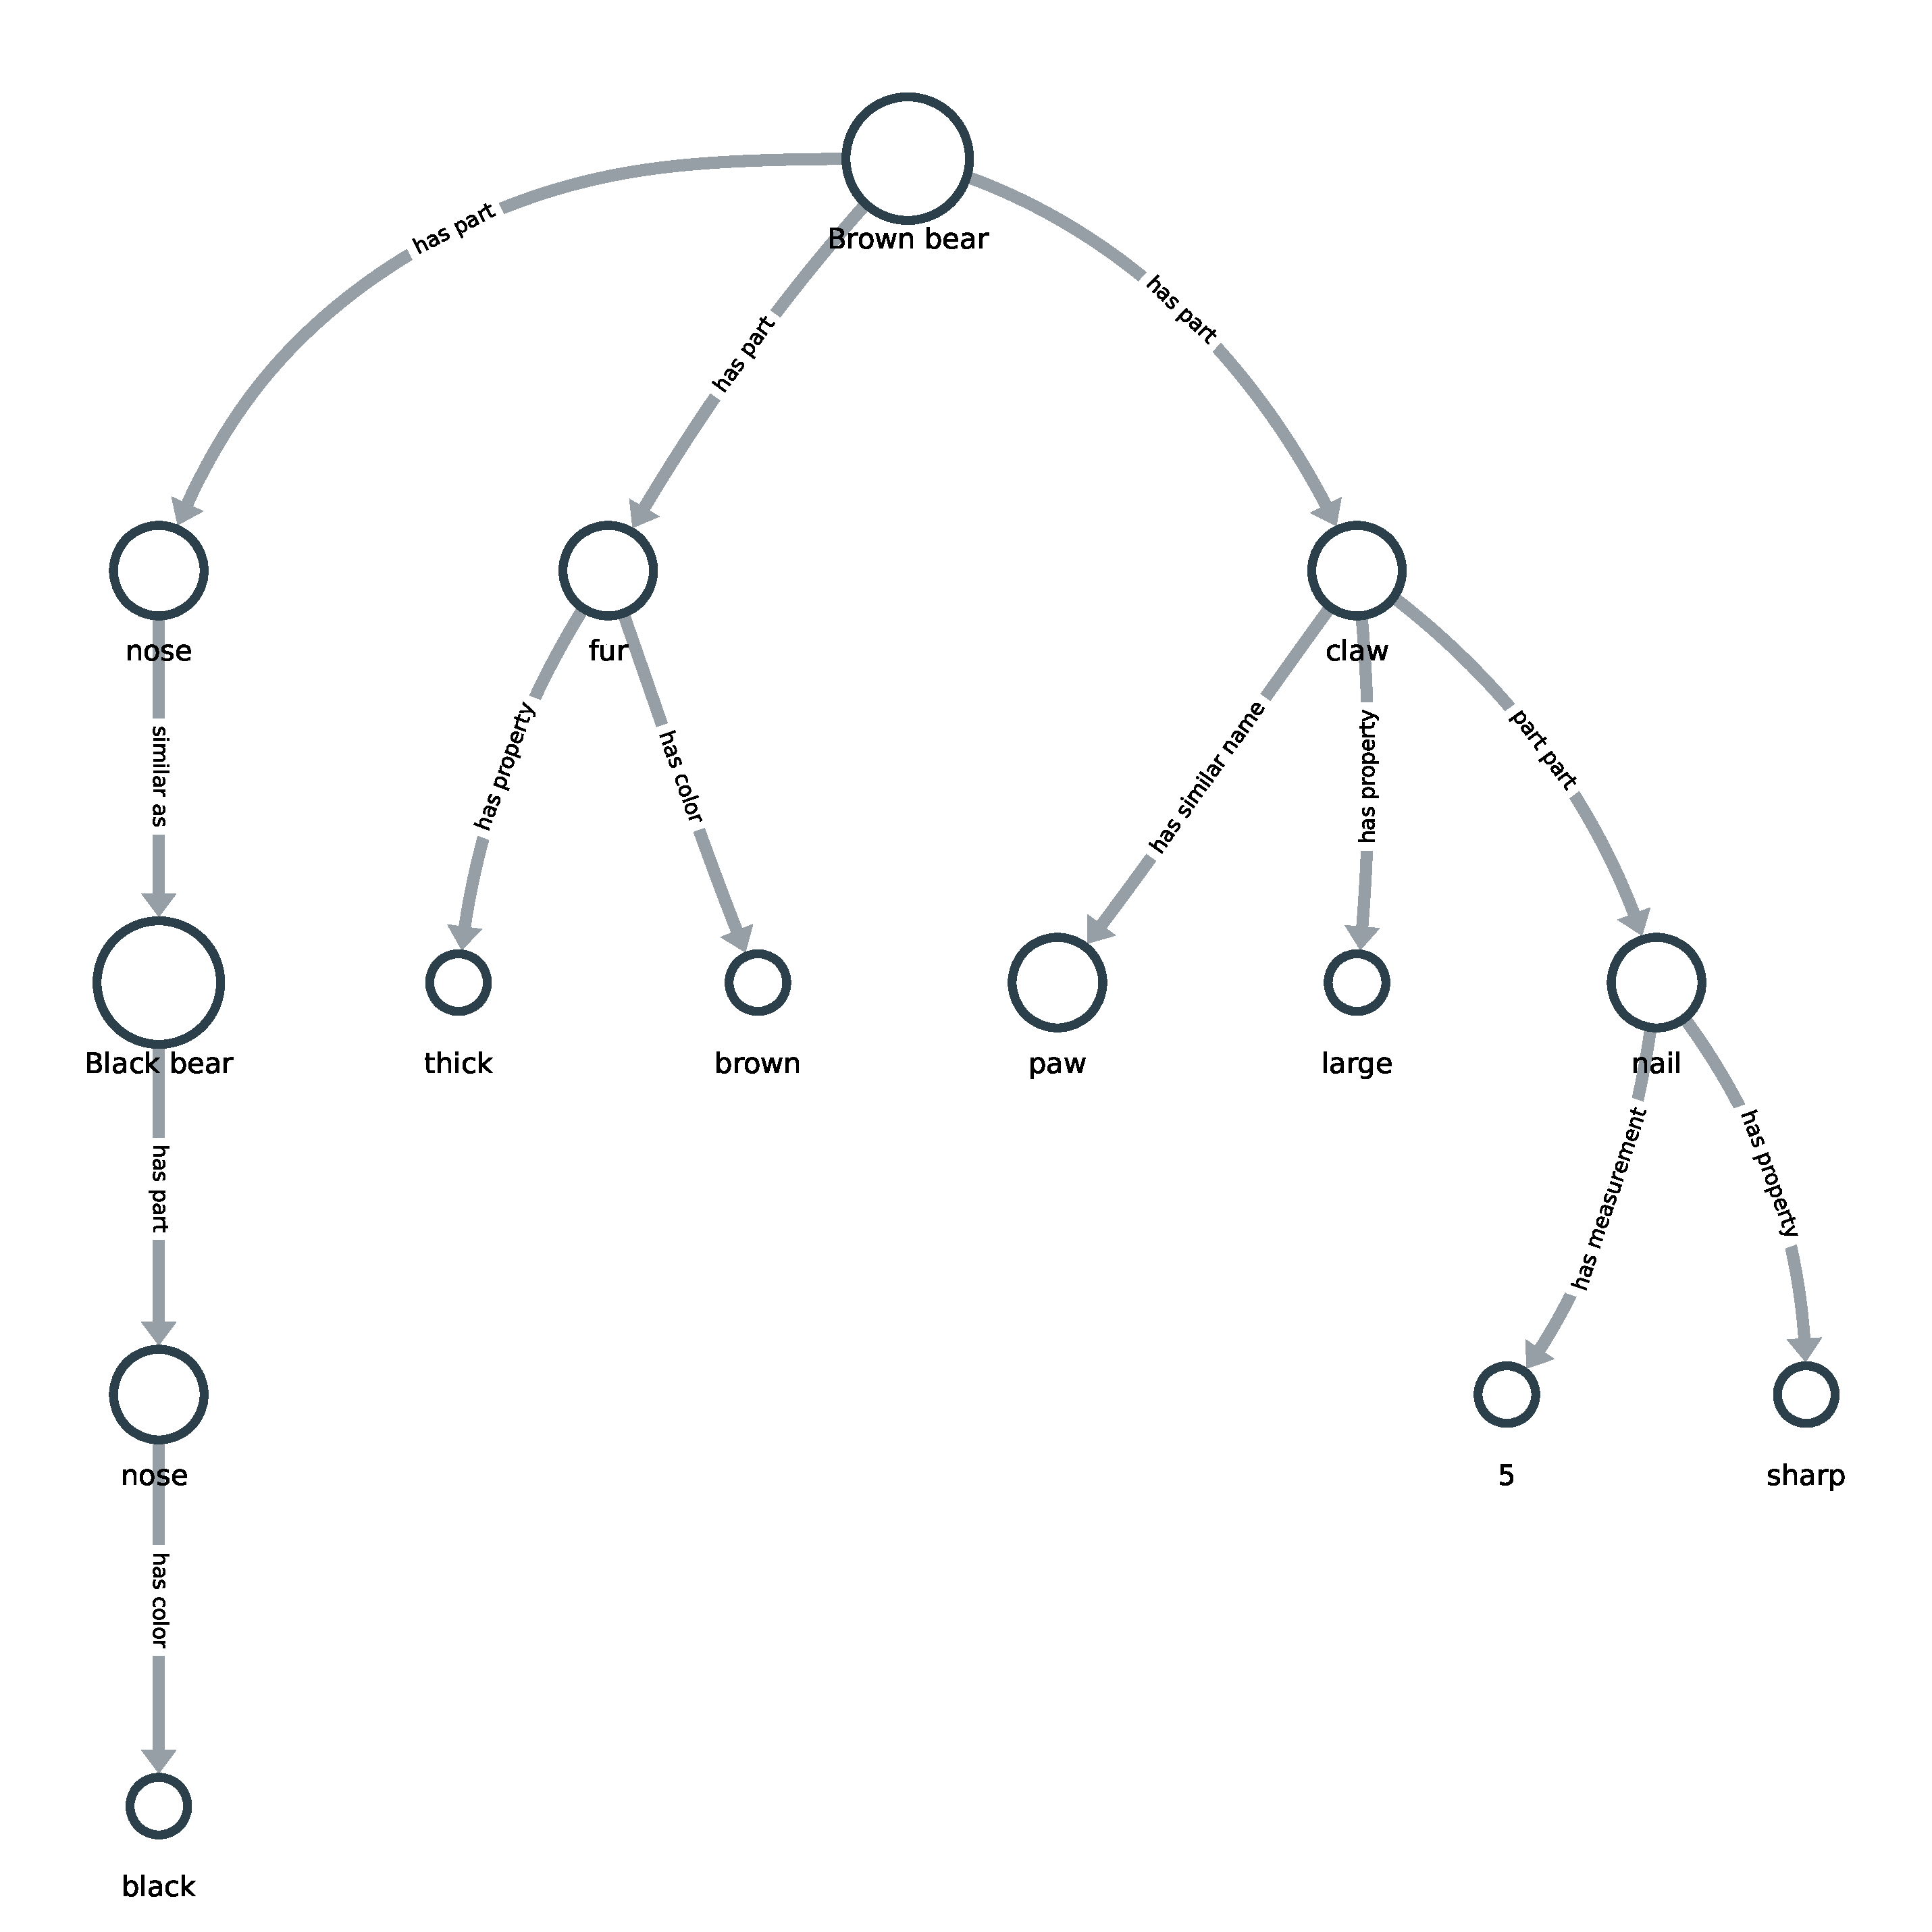
\includegraphics[width=\textwidth]{figures/kngraph_rec.pdf}
 \caption[Knowledge Graph Future Example]{An simple property knowledge graph. All the nodes consists of singular words; species can shared these traits. Relations are kept simple (simple property graph vs rigorous graph) and can be connected to other ontology's, like e.g. WikiData. The graph can also point towards other species in case the relation is 'similar to' and retrieve the correct traits.}
 \label{fig:kngraph_rec}
\end{figure}


\printbibliography
\newpage

\begin{subappendices}
\renewcommand{\thesection}{\arabic{section}}
\markboth{APPENDICES}{APPENDICES}

\section{Paragraph Description Key Words} \label{app:key_words}
\begin{table}[htpb]
\centering
\begin{tabular}{@{}lllll@{}}
Llifle       & AgroForestry & BoW            & PoWO                                                           & Wikipedia                                                             \\ \midrule
Description & Botanic      & Appearance     & \begin{tabular}[c]{@{}l@{}}General \\ Description\end{tabular} & \begin{tabular}[c]{@{}l@{}}General \\ description\end{tabular}        \\
            & Description  & Description    & Diagnostic                                                     & Description                                                           \\
            &              & Identification & Morphology                                                     & \begin{tabular}[c]{@{}l@{}}Physical \\ characteristics\end{tabular}   \\
            &              &                & Sex                                                            & \begin{tabular}[c]{@{}l@{}}Description and \\ morphology\end{tabular} \\
            &              &                & Sterile                                                        & Appearance                                                            \\
            &              &                & Fertile                                                        & Characteristics                                                       \\ \bottomrule
\end{tabular}
\label{tab:key_words}
\end{table}
\end{subappendices}

\backmatter

\end{document}